\documentclass[a4paper,11pt]{report}
\usepackage[hmargin=35mm,vmargin=35mm]{geometry}
\usepackage[utf8]{inputenc}
\usepackage[T1]{fontenc}

\overfullrule = 10mm

%-----------------------------------------------------------------------------
%	PACKAGES AND CONFIGURATION
%-----------------------------------------------------------------------------

\usepackage{amsmath,amssymb,amsthm,mathrsfs,amsfonts}
\usepackage{enumitem,microtype}
\usepackage{wrapfig,scalerel,relsize}
\usepackage[breakable]{tcolorbox}
\usepackage{graphicx,tikz,hyperref,cleveref}
\graphicspath{{graphics/}}
\usetikzlibrary{calc}
\hypersetup{
  colorlinks=true,
  linkcolor=blue,
  breaklinks=true,
  bookmarksnumbered=true,
  pdfauthor={Frederic P. Schuller, Simon Rea},
  pdfcreator={pdfLaTeX}
}

\newcommand\C{\mathbb{C}}
\newcommand\Q{\mathbb{Q}}
\newcommand\R{\mathbb{R}}
\newcommand\Z{\mathbb{Z}}
\newcommand\F{\mathbb{F}}
\newcommand\N{\mathbb{N}}
\renewcommand\H{\mathbb{H}}
\newcommand\cA{\mathcal{A}}
\newcommand\cF{\mathcal{F}}
\newcommand\cH{\mathcal{H}}
\newcommand\cJ{\mathcal{J}}
\newcommand\cK{\mathcal{K}}
\newcommand\cL{\mathcal{L}}
\newcommand\cO{\mathcal{O}}
\newcommand\cP{\mathcal{P}}

\DeclareMathOperator*{\slim}{s-lim}
\DeclareMathOperator*{\wlim}{w-lim}
\DeclareMathOperator{\AC}{AC}
\DeclareMathOperator{\Ad}{Ad}
\DeclareMathOperator{\Aut}{Aut}
\DeclareMathOperator{\ad}{ad}
\DeclareMathOperator{\Borel}{Borel}
\DeclareMathOperator{\Der}{Der}
\DeclareMathOperator{\Eig}{Eig}
\DeclareMathOperator{\End}{End}
\DeclareMathOperator*{\esup}{ess\,sup}
\DeclareMathOperator{\ev}{ev}
\DeclareMathOperator{\Gr}{Gr}
\DeclareMathOperator{\Hom}{Hom}
\DeclareMathOperator{\id}{id}
\DeclareMathOperator{\im}{im}
\DeclareMathOperator{\preim}{preim}
\DeclareMathOperator{\proj}{proj}
\DeclareMathOperator{\ran}{ran}
\DeclareMathOperator{\sgn}{sgn}
\DeclareMathOperator{\lspan}{span}
\DeclareMathOperator{\Tr}{Tr}
\DeclareMathOperator{\vol}{vol}
\DeclareMathOperator{\GL}{GL}
\DeclareMathOperator{\Ort}{O}
\DeclareMathOperator{\SO}{SO}
\DeclareMathOperator{\SU}{SU}
\DeclareMathOperator{\SL}{SL}

\newcommand\gl{\mathfrak{gl}}
\newcommand\ort{\mathfrak{o}}
\newcommand\so{\mathfrak{so}}
\newcommand\su{\mathfrak{su}}
\renewcommand\sl{\mathfrak{sl}}

\renewcommand\Re{\operatorname{Re}}
\renewcommand\Im{\operatorname{Im}}
\newcommand\ic{\mathrm{i}}
\newcommand\la{\langle}
\newcommand\ra{\rangle}
\newcommand\cl{\colon}
\renewcommand{\d}{\mathop{}\!\mathrm{d}}
\newcommand{\alev}{\mathrm{a.e.}}

\newcommand\Cal\mathcal

                         % custom macros
\usepackage[retainorgcmds]{IEEEtrantools} % I want to get rid of this

%-----------------------------------------------------------------------------
%	THEOREM STYLES
%-----------------------------------------------------------------------------

\newtheoremstyle{underline}% name
{}              % Space above, empty = `usual value'
{}              % Space below
{}              % Body font
{}              % Indent amount (empty = no indent, \parindent = para indent)
{}              % Thm head font
{.}             % Punctuation after thm head
{1.5mm}         % Space after thm head: \newline = linebreak
{{\underline{\textit{\thmname{#1}\thmnumber{ #2}}~\thmnote{(#3)}\unskip}}}  % Thm head spec

\theoremstyle{plain}
\newtheorem{theorem}{Theorem}[section]
\newtheorem{axiom}{Axiom}
\newtheorem{corollary}[theorem]{Corollary}
\newtheorem{lemma}[theorem]{Lemma}
\newtheorem{proposition}[theorem]{Proposition}

\theoremstyle{definition}
\newtheorem*{definition}{Definition}

\theoremstyle{remark}
\newtheorem*{notation}{Notation}
\newtheorem*{solution}{Solution}

\theoremstyle{underline}
\newtheorem{remark}[theorem]{Remark}
\newtheorem{example}[theorem]{Example}

\tcolorboxenvironment{theorem}{colframe=cyan,breakable}
\tcolorboxenvironment{corollary}{colframe=cyan,breakable}
\tcolorboxenvironment{lemma}{colframe=cyan,breakable}
\tcolorboxenvironment{proposition}{colframe=cyan,breakable}

\tcolorboxenvironment{definition}{colframe=lime,breakable}

\tcolorboxenvironment{example}{colframe=white,breakable}
\tcolorboxenvironment{remark}{colframe=white,breakable}
\tcolorboxenvironment{proof}{colframe=white,breakable}

%-----------------------------------------------------------------------------
%	MAIN DOCUMENT
%-----------------------------------------------------------------------------

\title{Lectures on Quantum Theory}
\author{Dr. Frederic P. Schuller \\ \small Notes by Simon Rea}
\date{Summer 2015}

\begin{document} 

  \maketitle 
  \tableofcontents

  \chapter*{Introduction}
  \addcontentsline{toc}{chapter}{Introduction}
  \input{00intro}

  \chapter{Axioms of quantum mechanics}
  \input{01axioms}

  \chapter{Banach spaces}
  
Hilbert spaces are a special type of a more general class of spaces
known as Banach spaces. We are interested in Banach spaces not just
for the sake generality, but also because they naturally appear in
Hilbert space theory. For instance, the space of bounded linear maps
on a Hilbert space is not itself a Hilbert space, but only a Banach
space.

\section{Generalities on Banach spaces}

We begin with some basis notions from metric space theory.

\begin{definition}
A \emph{metric space}\index{metric space} is a pair $(X,d)$, where $X$
is a set and $d$ is a \emph{metric} on $X$, that is, a map $d\cl
X\times X \to [0,\infty)$ satisfying
\begin{enumerate}[label=(\roman*)]
\item $d(x,y) = 0\ \Leftrightarrow \ x=y$ \hfill (identity of indiscernibles)
\item $d(x,y)=d(y,x)$ \hfill (symmetry)
\item $d(x,z)\leq d(x,y)+d(y,z)$ \hfill (triangle inequality)
\end{enumerate}
for all $x,y,z\in X$.
\end{definition}

\begin{definition}
A sequence $\{x_n\}_{n\in \N}$ in a metric space $(X,d)$ is said to
\emph{converge}\index{convergence} to an element $x\in X$, written
$\displaystyle \lim_{n\to \infty}x_n=x$, if
\begin{equation*}
\forall \, \varepsilon > 0 : \exists \, N \in \N : \forall \, n \geq N : \ d(x_n,x)<\varepsilon.
\end{equation*}
\end{definition}

A sequence in a metric space can converge to at most one element.

\begin{definition}
A \emph{Cauchy sequence}\index{Cauchy sequence} in a metric space $(X,d)$ is a sequence $\{x_n\}_{n\in \N}$ such that
\begin{equation*}
\forall \, \varepsilon > 0 : \exists \, N \in \N : \forall \, n,m \geq N : \ d(x_n,x_m)<\varepsilon.
\end{equation*}
\end{definition}
Any convergent sequence is clearly a Cauchy sequence.

\begin{definition}
A metric space $(X,d)$ is said to be \emph{complete}\index{completeness} if every Cauchy sequence converges to some $x\in X$.
\end{definition}
A natural metric on a vector space is that induced by a norm.
\begin{definition}
A \emph{normed space}\index{normed space} is a (complex) vector space
$(V,+,\cdot)$ equipped with a \emph{norm}, that is, a map
$\|\cdot\|\cl V \to [0,\infty)$ satisfying
\begin{enumerate}[label=(\roman*)]
\item $\|f\| = 0 \ \Leftrightarrow\ f=0$ \hfill (positive definiteness)
\item $\|z\cdot f\|=|z|\|f\|$ \hfill (homogeneity/scalability)
\item $\|f+g\|\leq \|f\|+\|g\|$ \hfill (triangle inequality/sub-additivity)
\end{enumerate}
for all $f,g\in V$ and all $z\in \C$.
\end{definition}
One we have a norm $\|\cdot\|$ on $V$, we can define a metric $d$ on $V$ by 
\begin{equation*}
d(f,g) := \|f-g\|.
\end{equation*}
Then we say that the normed space $(V,\|\cdot\|)$ is \emph{complete} if the metric space $(V,d)$, where $d$ is the metric induced by $\|\cdot\|$, is complete. Note that we will usually suppress inessential information in the notation, for example writing $(V,\|\cdot\|)$ instead of $(V,+,\cdot,\|\cdot\|)$.

\begin{definition}
A \emph{Banach space}\index{Banach space} is a complete normed vector space.
\end{definition}

\begin{example}
  The set of continuous functions
  \begin{equation}
    C^0_\C[0,1]:=\{f\cl [0,1]\to \C \mid f \text{ is continuous}\}
  \end{equation}
  is a vector space with the pointwise sum and scalar product (meaning
  that the sum and product of continuous functions is again continuous).
  Since $[0,1]$ is closed and bounded, it is compact and hence
  every complex-valued continuous function $f\cl [0,1]\to \C$ is
  bounded, in the sense that the supremum
  \begin{equation}
    \|f\|_\infty = \sup \{|f(x)|\mid x\in[0,1]\}
  \end{equation}
  is always finite.
  We claim that this function defines a norm on $C^0_\C[0,1]$,
  called the \emph{supremum} (or \emph{infinity}) \emph{norm},
  and that, equipped with this norm, the space \(C^{0}_\C[0,1]\) is
  complete (i.e. it is a Banach space).
  Let us show this in some detail.

  The function \(\|.\|_\infty\) is clearly positive definite, so to
  see that it is a norm, it remains to show homogeneity and the
  triangle inequality.
  Let $f,g\in C^0_\C[0,1]$ and $z\in \C$. Then we have
  \begin{align}
    \|z\cdot f\|_{\infty}
    &:= \sup_{x\in[0,1]}|zf(x)| \\
    &= \sup_{x\in[0,1]}|z||f(x)| \\
    & =|z|\sup_{x\in[0,1]}|f(x)| \\
    &= |z|\|f\|_{\infty}
  \end{align}
  and
  \begin{align*}
  \|f+g\|_{\infty}
  &:= \sup_{x\in[0,1]}|(f+g)(x)|\\
  &= \sup_{x\in[0,1]}|f(x)+g(x)|\\
  &\leq \sup_{x\in[0,1]}(|f(x)|+|g(x)|)\\
  & = \sup_{x\in[0,1]}|f(x)|\,+\sup_{x\in[0,1]}|g(x)|\\
  & = \|f\|_{\infty}+\|g\|_{\infty}.
  \end{align*}
  Hence, $(C^0_\C[0,1],\|\cdot\|_{\infty})$ is indeed a normed space.
  We now show that $C^0_\C[0,1]$ is complete. Let $\{f_n\}_{n\in \N}$ be
  a Cauchy sequence of functions in $C^0_\C[0,1]$, that is
  \begin{equation*}
    \forall \, \varepsilon > 0 :
    \exists \, N \in \N :
    \forall \, n,m \geq N :
    \ \|f_n-f_m\|_{\infty} <\varepsilon.
  \end{equation*}
  We seek an $f\in C^0_\C[0,1]$ such that $\displaystyle
  \lim_{n\to\infty}f_n=f$. We will proceed in three steps.
  \begin{enumerate}
    \item
      We first define a candidate function \(f\).
      Fix $y\in [0,1]$ and $\varepsilon >0$. By definition of supremum, we have
      \begin{equation*}
      |f_n(y) -f_m(y)|
      \leq \sup_{x\in[0,1]}|f_n(x)-f_m(x)|
      =: \|f_n-f_m\|_{\infty}.
      \end{equation*}
      Hence, there exists $N\in \N$ such that
      \begin{equation*}
      \forall \, n,m \geq N : \ |f_n(y) -f_m(y)|<\varepsilon,
      \end{equation*}
      that is, the sequence of complex numbers $\{f_n(y)\}_{n\in \N}$ is a
      Cauchy sequence. Since $\C$ is a complete metric space,
      the sequence \(f_n(y)\) converges. Thus, we can define a function
      \begin{align*}
      f\cl [0,1] & \to \C
      \\
      x & \mapsto \lim_{n\to\infty}f_n(x),
      \end{align*}
      called the \emph{pointwise limit} of $f$.
      Note that, even if \(f(x)=\lim_{n\to\infty}f_n(x)\), this does
      \emph{not} automatically imply that $\lim_{n\to
      \infty}f_n=f$ (convergence with respect to the supremum norm), nor that
      $f\in C^0_\C[0,1]$, and hence we need to check separately that these
      do, in fact, hold.
    \item
      Let us check that $f$ is continuous, i.e.
      that for every \(\epsilon>0\), there is some \(\delta>0\) such that
      \begin{equation}
        |x-y|<\delta \implies |f(x)-f(y)|<\epsilon
      .\end{equation}
      For any \(n\in \N\), we have
      \begin{align*}
      |f(x)-f(y)|
      & = |f(x)-f_n(x)+f_n(x)-f_n(y)+f_n(y)-f(y)|
      \\
      & \leq |f(x)-f_n(x)|+|f_n(x)-f_n(y)|+|f_n(y)-f(y)|.
      \end{align*}
      Note that the summand in the middle can be bound by \(\epsilon /
      3\) by taking \(\delta\) small enough.
      The main challenge is that the other two summands are bounded
      separately for each point, e.g. for each \(x\) there is \(N_x\)
      such that
      \begin{equation}
        |f(x)-f_{N_x}(x)|<\frac{\epsilon}{3}
      .\end{equation}
      If we could find a single \(N\) that works for all \(x\) at
      once, we would have
      \begin{align*}
      |f(x)-f(y)|
      & \leq \frac{\epsilon}{3} + |f_N(x)-f_N(y)|+\frac{\epsilon}{3}
      \end{align*}
      so by continuity of \(f_N\) there is a \(\delta>0\) such that
      \(|f_N(x)-f_N(y)|<\epsilon / 3\), wich implies the result.

      It is the Cauchy property of \(\{f_n\}\) that comes to save the day.
      There is an \(N\in\N\) such that
      \begin{equation}
        \forall x\in[0,1], \ \forall m,n\geq N,\ |f_m(x)-f_n(x)| <
        \epsilon / 4
      \end{equation}
      Taking \(n=N\) and \(m\to\infty\), we obtain
      \begin{equation}
        \forall x\in[0,1], \ |f(x)-f_N(x)|\leq \epsilon / 4 < \epsilon /
        3,
      \end{equation}
      which is what we needed.
    \item
      Finally, it remains to show that $\lim_{n\to \infty}f_n=f$ or,
      equivalently, \(\lim_{n\to\infty}\|f-f_n\|=0\).
      Given \(\epsilon>0\), we must show that there is \(N\) such that
      \begin{equation}
        \forall n\geq N,\ \|f-f_n\| < \epsilon
      .\end{equation}
      The Cauchy property of \(\{f_n\}\) tells us
      that there is \(N\geq 0\) with
      \begin{equation}
        \forall m,n\geq N,\ \|f_m-f_n\|<\epsilon / 2
      .\end{equation}
      This implies that
      \begin{equation}
        \forall x\in[0,1],\ \forall m,n\geq N,\ |f_m(x)-f_n(x)|<\epsilon
        / 2
      .\end{equation}
      Taking the limit \(m\to\infty\), we get
      \begin{equation}
        \forall x\in[0,1],\ \forall n\geq N,\ |f(x)-f_n(x)|\leq \epsilon
        / 2
      \end{equation}
      so, for all \(n\geq N\), we have \(\|f-f_n\|\leq
      \frac{\epsilon}{2}<\epsilon \), as we wanted.
  \end{enumerate}
  This completes the proof that $(C^0_\C[0,1],\|\cdot\|_{\infty})$ is a
  Banach space.
\end{example}

\begin{remark}
The previous example shows that checking that something is a Banach space, and the completeness property in particular, can be quite tedious. However, in the following, we will typically already be working with a Banach (or Hilbert) space and hence, rather than having to check that the completeness property holds, we will instead be able to use it to infer the existence (within that space) of the limit of any Cauchy sequence.
\end{remark}

\section{Bounded linear operators}

As usual in mathematics, once we introduce a new types of structure,
we also want study maps between instances of those structures, with
extra emphasis placed on the structure-preserving maps.
We begin with linear maps between normed spaces.

\begin{proposition}
\label{prp:boundequiv}
Let $(V,\|\cdot\|_V)$, $(W,\|\cdot\|_W)$ be normed spaces
and $A\cl V\to W$ a linear operator.
The following conditions are equivalent.
\begin{enumerate}[label=(\roman*)]
  \item \(\displaystyle \sup_{f\in V-\{0\}}\frac{\|Af\|_W }{ \|f\|_V}
    < \infty\)
  \item $\displaystyle \sup_{\|f\|_V=1}\|Af\|_W< \infty$
  \item $\exists \, k > 0 : \forall \, f\in V: \ \|f\|_V \leq 1\, \Rightarrow \, \|Af\|_W \leq k$
  \item $\exists \, k > 0 : \forall \, f\in V: \ \|Af\|_W\leq  k \|f\|_V$
  \item the map $A\cl V \to W$ is continuous with respect to the topologies induced by the respective norms on $V$ and $W$
  \item the map $A$ is continuous at $0\in V$. 
\end{enumerate}
Moreover, in this case, the following numbers are equal:
\begin{itemize}
  \item \(\sup\left\{\frac{\|Af\|}{\|f\|} \mid f\in V-\{0\}\right\}\)
  \item \(\sup \{\|Af\| : f\in V, \|f\|=1\}\)
  \item \(\sup \{\|Af\| : f\in V, \|f\|\leq 1\}\)
  \item \(\inf \{C\in[0,\infty) \mid \forall f\in V, \|Af\|\leq C\|f\|\}\)
\end{itemize}
\end{proposition}

\begin{definition}
  Let \(V,W\) be normed spaces.
  A linear operator $A\cl V\to W$ is said to be \emph{bounded} if it
  satisfies the conditions in the previous proposition.
  If $A\cl V \to W$ is a bounded operator, the \emph{operator
  norm}\index{operator norm} \(\|A\|\) of $A$ is the number given by
  any of the three suprema or the infimum in the proposition.
\end{definition}

\begin{remark}
  The set of \(C\in[0,\infty)\) with \(\|Af\|\leq C\|f\|\) for all
  \(f\in V\) is a closed set in \(\R\).
  Indeed, if \(C_n\) is a sequence in the set, we have \(\|Af\|\leq
  C_n\|f\|\), so \(\|Af\|\leq\lim_{n\to\infty}C_n\|f\|\).
  Then, the operator norm \(\|A\|\) is actually the \emph{minimum} of
  this set, meaning that
  \begin{equation}
    \forall f\in V, \|Af\|\leq\|A\|\|f\|
  .\end{equation}
\end{remark}

\begin{example}
Let $\id_W\cl W\to W$ be the identity operator on a Banach space $W$. Then
\begin{equation*}
\sup_{f\in W}\frac{\|\id_Wf\|_W}{\|f\|_W} =\sup_{f\in W}1 = 1 <\infty.
\end{equation*}
Hence, $\id_W$ is a bounded operator and has unit norm.
\end{example}

\begin{example}
Denote by $C^1_{\C}[0,1]$ the complex vector space of once continuously differentiable complex-valued functions on $[0,1]$. Since differentiability implies continuity, this is a subset of $C^0_{\C}[0,1]$. Moreover, since sums and scaling by a complex number of continuously differentiable functions are again continuously differentiable, this is, in fact, a vector subspace of $C^0_{\C}[0,1]$, and hence also a normed space with the supremum norm $\|\cdot\|_{\infty}$.

Consider the first derivative operator
\begin{align*}
D \cl C^1_{\C}[0,1] & \to C^0_{\C}[0,1]\\
 f & \mapsto f'.
\end{align*}
We know from undergraduate real analysis that $D$ is a linear operator. We will now show that $D$ is an unbounded\footnote{Some people take the term unbounded to mean ``not necessarily bounded''. We take it to mean ``definitely not bounded'' instead.} linear operator. That is,
\begin{equation*}
\sup_{f\in C^1_{\C}[0,1]} \frac{\|Df\|_{\infty}}{\|f\|_{\infty}} = \infty.
\end{equation*}
Note that, since the norm is a function into the real numbers, both $\|Df\|_{\infty}$ and $\|f\|_{\infty}$ are always finite for any $f\in C^1_{\C}[0,1]$. Recall that the supremum of a set of real numbers is its least upper bound and, in particular, it need not be an element of the set itself. What we have to show is that the set
\begin{equation*}
\biggl\{ \frac{\|Df\|_{\infty}}{\|f\|_{\infty}} \ \Big| \ f\in C^1_{\C}[0,1] \biggr\} \subset \R
\end{equation*}
contains arbitrarily large elements. One way to do this is to exhibit a positively divergent (or unbounded from above) sequence within the set. 

Consider the sequence $\{f_n\}_{n\geq 1}$ where $f_n(x):=\sin(2\pi nx)$. We know that sine is continuously differentiable, hence $f_n\in C^1_{\C}[0,1]$ for each $n\geq 1$, with
\begin{equation*}
Df_n(x) = D(\sin(2\pi nx)) = 2\pi n\cos(2\pi nx).
\end{equation*}
We have
\begin{equation*}
\|f_n\|_{\infty} = \sup_{x\in[0,1]}|f_n(x)| = \sup_{x\in[0,1]}|\sin(2\pi nx)| = \sup \, [-1,1] = 1 
\end{equation*}
and
\begin{equation*}
\|Df_n\|_{\infty} = \sup_{x\in[0,1]}|Df_n(x)| = \sup_{x\in[0,1]}|2\pi n\cos(2\pi nx)| = \sup\, [-2\pi n,2\pi n] = 2\pi n.
\end{equation*}
Hence, we have
\begin{equation*}
\sup_{f\in C^1_{\C}[0,1]} \frac{\|Df\|_{\infty}}{\|f\|_{\infty}} \geq \sup_{\{f_n\}_{n\geq 1}} \frac{\|Df\|_{\infty}}{\|f\|_{\infty}} = \sup_{n\geq 1}\,2\pi n = \infty,
\end{equation*}
which is what we wanted. As an aside, we note that $C^1_{\C}[0,1]$ is not complete with respect to the supremum norm, but it is complete with respect to the norm
\begin{equation*}
\|f\|_{C^1}:=\|f\|_{\infty}+\|f'\|_{\infty}.
\end{equation*}
While the derivative operator is still unbounded with respect to this new norm, in general, the boundedness of a linear operator does depend on the choice of norms on its domain and target, as does the numerical value of the operator norm.
\end{example}

\begin{remark}
Apart from the ``minor'' detail that in quantum mechanics we deal with Hilbert spaces, use a different norm than the supremum norm and that the (one-dimensional) momentum operator acts as $P(\psi):=-\mathrm{i}\hbar\psi'$, the previous example is a harbinger of the fact that the momentum operator in quantum mechanics is unbounded. This will be the case for the position operator $Q$ as well.
\end{remark}

\begin{lemma}
\label{lem:forcompl}
Let $(V,\|\cdot\|)$ be a normed space. Then, addition, scalar
multiplication, and the norm are all sequentially continuous. That is,
for any sequences $\{f_n\}_{n\in \N}$ and $\{g_n\}_{n\in \N}$ in $V$
converging to $f\in V$ and $g\in V$ respectively, and any sequence
$\{z_n\}_{n\in \N}$ in $\C$ converging to $z\in \C$, we have
\begin{enumerate}[label=(\roman*)]
\item $\displaystyle \lim_{n\to \infty}(f_n+g_n)=f+g$
\item $\displaystyle \lim_{n\to \infty}z_nf_n=zf$.
\item $\displaystyle \lim_{n\to \infty}\|f_n\|=\|f\|$
\end{enumerate}
\end{lemma}

\iffalse
\begin{proof}
\begin{enumerate}[label=(\roman*)]
\item Let $\varepsilon >0$. Since $\displaystyle \lim_{n\to \infty}f_n=f$ and $\displaystyle \lim_{n\to \infty}g_n=g$ by assumption, there exist $N_1,N_2\in \N$ such that
\begin{align*}
  \forall \, n\geq N_1, & \ \|f-f_n\|<\tfrac{\varepsilon}{2}\phantom{.}\\
  \forall \, n\geq N_2, & \ \|g-g_n\|<\tfrac{\varepsilon}{2}.
\end{align*}
Let $N:=\max\{N_1,N_2\}$. Then, for all $n\geq N$, we have
\begin{align*}
\|(f_n+g_n)-(f+g)\|
&= \|f_n-f+g_n-g\|\\
&\leq \|f_n-f\|+\|g_n-g\|\\
& < \tfrac{\varepsilon}{2}+\tfrac{\varepsilon}{2}\\
& = \varepsilon.
\end{align*}
Hence $\displaystyle \lim_{n\to \infty}(f_n+g_n)=f+g$.


\item Since $\{z_n\}_{n\in \N}$ is a convergent sequence in $\C$, it is bounded. That is,
\begin{equation*}
\exists \, k>0 : \forall \, n\in \N : \ |z_n|\leq k.
\end{equation*}
Let $\varepsilon >0$. Since $\displaystyle \lim_{n\to \infty}f_n=f$ and $\displaystyle \lim_{n\to \infty}z_n=z$, there exist $N_1,N_2\in \N$ such that
\begin{align*}
  \forall \, n\geq N_1, & \ \|f-f_n\|<\frac{\varepsilon}{2k}\\
  \forall \, n\geq N_2, & \ \|z-z_n\|<\frac{\varepsilon}{2\|f\|}.
\end{align*}
Let $N:=\max\{N_1,N_2\}$. Then, for all $n\geq N$, we have
\begin{align*}
\|z_nf_n-zf\|
&= \|z_nf_n-z_nf+z_nf-zf\|\\
&= \|z_n(f_n-f)+(z_n-z)f\|\\
&\leq \|z_n(f_n-f)\|+\|(z_n-z)f\|\\
&= |z_n|\|f_n-f\|+|z_n-z|\|f\|\\
& < k\frac{\varepsilon}{2k}+\frac{\varepsilon}{2\|f\|}\|f\|\\
& = \varepsilon.
\end{align*}
Hence $\displaystyle \lim_{n\to \infty}z_nf_n=zf$.
\item Let $\varepsilon >0$. Since  $\displaystyle \lim_{n\to \infty}f_n=f$, there exists $N\in \N$ such that
\begin{equation*}
\forall \, n \geq N : \ \|f_n-f\|<\varepsilon.
\end{equation*}
By the triangle inequality, we have
\begin{equation*}
\|f_n\| = \|f_n-f+f\| \leq \|f_n-f\|+\|f\|  
\end{equation*}
so that $\|f_n\|-\|f\|\leq \|f_n-f\|$. Similarly, $\|f\|-\|f_n\|\leq \|f-f_n\|$. Since
\begin{equation*}
\|f-f_n\| = \|-(f_n-f)\| = |-1|\|f_n-f\| = \|f_n-f\|,
\end{equation*}
we have $-\|f_n-f\|\leq\|f_n\|-\|f\|\leq\|f_n-f\|$ or, by using the modulus,
\begin{equation*}
\bigl| \|f_n\|-\|f\|\bigr| \leq \|f_n-f\|.
\end{equation*}
Hence, for all $n\geq N$, we have $\bigl| \|f_n\|-\|f\|\bigr| <\varepsilon$ and thus  $\displaystyle \lim_{n\to \infty}\|f_n\|=\|f\|$.
\qedhere
\end{enumerate}
\end{proof}
\fi
Note that by taking $\{z_n\}_{n\in\N}$ to be the constant sequence whose terms are all equal to some fixed $z\in \C$, we have $\displaystyle \lim_{n\to \infty}zf_n=zf$ as a special case of (ii).

This lemma will take care of some of the technicalities involved in proving the following crucially important result.

\begin{theorem}
Let \(V,W\) be normed spaces. Then the set $\mathcal{L}(V,W)$ of
bounded linear operators, equipped with the operator norm, is a normed space.
Moreover, if \(W\) is Banach, then \(\Cal L(V,W)\) is Banach.
\end{theorem}

\begin{proof}
Define addition and scalar multiplication on $\mathcal{L}(V,W)$ by
\begin{equation*}
(A+B)f := Af+Bf \quad \qquad (zA)f := zAf.
\end{equation*}
It is clear that both $A+B$ and $zA$ are linear operators, so this
addition and scalar multiplication are operations
\begin{align*}
  +\cl \mathcal{L}(V,W)\times \mathcal{L}(V,W) & \to\mathcal{L}(V,W)
  &
  \cdot \cl \C \times \mathcal{L}(V,W) & \to \mathcal{L}(V,W)\\
  (A,B) & \mapsto A+B 
        &
  (z,A) & \mapsto zA
\end{align*}
and one checks that they give \(\Cal L(V,W)\) the structure
of a vector space.
Now we will see that it is a Banach space with the operator norm.
We start by checking that the ``operator norm'' \emph{is} a norm on \(\Cal
L(V,W)\).
\begin{enumerate}[label=(\alph*)]
\item
  We have
  \begin{align*}
    \|(A+B)f\|_W
    &:= \|Af+Bf\|_W \\
    &\leq \|Af\|_W+\|Bf\|_W \\
    &\leq \|A\|\|f\| + \|B\|\|f\| \\
    &= (\|A\|+ \|B\|)\|f\|
  \end{align*}
  since $A$ and $B$ are bounded. Hence, $A+B$ is also bounded and we have
  \begin{equation*}
  \|A+B\|\leq \|A\|+\|B\|.
  \end{equation*}
  \item
  Similarly, for $z\in\C$ and \(A\in\Cal L(V,W)\), we have 
  \begin{align*}
    \|(zA)f\|_W
    &:= \|zAf\|_W \\
    &= |z|\|Af\|_W \\
    &\leq |z|\|A\|\|f\|_W
  \end{align*}
  since $A$ is bounded and $|z|$ is finite.
  Hence, $zA$ is bounded.  and we have
  \begin{equation*}
  \|zA\|=|z|\|A\|.
  \end{equation*}
  \item
    $\displaystyle \|A\|:=\sup_{f\in
    V}\frac{\|Af\|_W}{\|f\|_V}\geq 0$ since $\|\cdot\|_V$ and
    $\|\cdot\|_W$ are norms.
  \item Again, by using the fat that $\|\cdot\|_W$ is a norm,
  \begin{align*}
  \|A\|=0
  & \iff \sup_{f\in V}\frac{\|Af\|_W}{\|f\|_V}= 0 \\
  & \iff \forall \, f\in V:\ \|Af\|_W=0\\
  & \iff \forall \, f\in V:\ Af=0\\
  & \iff A=0.
  \end{align*}
Hence, $(\mathcal{L}(V,W),\|\cdot\|)$ is a normed space.
\end{enumerate}
Now suppose that \(W\) is complete.
We will show that $\Cal{L}(V,W)$ is also complete.
We will proceed in three steps, analogously to the case of $C_{\C}^0[0,1]$.
\begin{enumerate}[label=(c.\roman*)]
\item Let $\{A_n\}_{n\in \N}$ be a Cauchy sequence in
  $\mathcal{L}(V,W)$. Fix $f\in V$ and let $\varepsilon >0$. Then,
  there exists $N\in \N$ such that
  \begin{equation*}
  \forall \, n,m\geq N : \ \|A_n-A_m\|<\frac{\varepsilon}{\|f\|_V}.
  \end{equation*}
  Then, for all $n,m\geq N$, we have
  \begin{equation*}
  \|A_nf-A_mf\|_W
  \leq \|f\|_V\|A_n-A_m\|\\
  < \varepsilon.
  \end{equation*}
  (Note that if $f=0$, we simply have $\|A_nf-A_mf\|_W=0<\varepsilon$
  and, in the future, we will not mention this case explicitly.) Hence,
  the sequence $\{A_nf\}_{n\in \N}$ is a Cauchy sequence in $W$. Since
  $W$ is a Banach space, the limit $\lim_{n\to \infty}A_nf$ exists and
  is an element of $W$. Thus, we can define the operator
  \begin{align*}
  A\cl V & \to W\\
  f & \mapsto \lim_{n\to \infty}A_nf,
  \end{align*}
  called the pointwise limit of $\{A_n\}_{n\in \N}$.
\item We now show that $A\in \mathcal{L}(V,W)$. This is where
  the previous lemma comes in handy. For linearity, let $f,g\in V$ and
  $z\in \C$. Then
  \begin{align*}
  A(zf+g) &:= \lim_{n\to \infty} A_n(zf+g)\\
  & = \lim_{n\to \infty} (zA_nf+A_ng)\\
  & = z\lim_{n\to \infty} A_nf+\lim_{n\to \infty}A_ng\\
  &=: zAf+Ag
  \end{align*}
  where we have used the linearity of each $A_n$ and part (i) and (ii)
  of \Cref{lem:forcompl}.
  Now we prove that \(A\) is bounded.
  First recall that $\{A_n\}_{n\in \N}$ is a Cauchy sequence. It
  follows that \(\{\|A_n\|\}_{n\in\N}\) is also Cauchy. Indeed, for
  \(\epsilon>0\) there exists $N\in \N$ such that
  \begin{equation*}
  \forall \, n,m \geq N : \ \|A_n-A_m\|<\varepsilon.
  \end{equation*}
  It follows that
  \begin{equation*}
  \bigl| \|A_n\|-\|A_m\|\bigr| \leq  \|A_n-A_m\|<\varepsilon
  \end{equation*}
  for all $n,m \geq N$.
  Since \(\R\) is complete, \(\{\|A_n\|\}_{n\in\N}\) converges to a
  finite \(r\).
  Now, by part (ii) and (iii) of \Cref{lem:forcompl}, we get
  \begin{align*}
  \|Af\|_W  & = \lim_{n\to \infty} \|A_nf\|_W\\
  & \leq \lim_{n\to \infty} \|A_n\|_W\|f\|_V \\
  & = \|f\|_V \lim_{n\to \infty} \|A_n\|
  \end{align*}
  for any $f\in V$.
  It follows that \(A\) is bounded and
  \begin{equation*}
  \|A\|\leq \lim_{n\to \infty} \|A_n\|
  \end{equation*}

\item
  To conclude, we show that $A_n\to A$.
  Let $\varepsilon >0$. 
  Since $\{A_n\}_{n\in \N}$ is Cauchy, there exists $N\in \N$ such that
  \begin{equation*}
  \forall \, n,m\geq N : \ \|A_n-A_m\| < \epsilon.
  \end{equation*}
  Hence, for any \(f\in V\), we have
  \begin{equation}
    \|A_nf-A_mf\|\leq \|A_n-A_m\|\|f\| <\epsilon\|f\|
  .\end{equation}
  Taking \(m\to\infty\), we get
  \begin{equation}
    \|A_nf-Af\|\leq \epsilon\|f\|
  \end{equation}
  for all \(f\in V\).
  This shows that \(\|A_n-A\|\leq\epsilon\). Since \(\epsilon>0\) is
  arbitrary, we conclude \(\|A_n-A\|\to 0\), so \(A_n\to A\).
\end{enumerate}
This concludes the proof that $(\mathcal{L}(V,W),\|\cdot\|)$ is a Banach space.
\end{proof}

The following is an extremely important special case of $\mathcal{L}(V,W)$.

\begin{definition}
Let $V$ be a normed space. Then $V^*:=\mathcal{L}(V,\C)$ is called the \emph{dual}\index{dual} of $V$.
\end{definition}

Note that, since $\C$ is a Banach space, the dual of a normed space is a Banach space. The elements of $V^*$ are variously called \emph{covectors} or \emph{functionals} on $V$. 
\begin{remark}
You may recall from undergraduate linear algebra that the dual of a vector space was defined to be the vector space of \emph{all} linear maps $V\to\C$, rather than just the bounded ones. This is because, in finite dimensions, all linear maps are bounded. So the two definitions agree as long as we are in finite dimensions. If we used the same definition for the infinite-dimensional case, then $V^*$ would lack some very desirable properties, such as that of being a Banach space.
\end{remark}
The dual space can be used to define a weaker notion of convergence called, rather unimaginatively, weak convergence. 

\begin{definition}
A sequence $\{f_n\}_{n\in \N}$ is said to \emph{converge
weakly}\index{weak convergence} to $f\in V$ if the sequence of complex
numbers $\{\varphi(f_n)\}_{n\in \N}$ converges to \(\varphi(f)\) for
every linear functional \(\varphi\):
\begin{equation*}
\forall \, \varphi\in V^* : \lim_{n\to\infty}\varphi(f_n) = \varphi(f).
\end{equation*}
To indicate that the sequence $\{f_n\}_{n\in \N}$ converges weakly to
$f\in V$ we write
\begin{equation*}
\wlim_{n\to \infty} f_n = f.
\end{equation*}
\end{definition}

In order to further emphasise the distinction with weak convergence,
we may say that $\{f_n\}_{n\in \N}$ converges \emph{strongly} to $f\in
V$ if it converges according to the usual definition, and we will
write accordingly
\begin{equation*}
\slim_{n\to \infty} f_n = f.
\end{equation*}

\begin{proposition}
Let $\{f_n\}_{n\in \N}$ be a sequence in a normed space $(V,\|\cdot\|_V)$. If $\{f_n\}_{n\in \N}$ converges strongly to $f\in V$, then it also converges weakly to $f\in V$, i.e.\
\begin{equation*}
\slim_{n\to \infty} f_n = f \quad \Rightarrow \quad \wlim_{n\to \infty} f_n = f.
\end{equation*}
\end{proposition}

\begin{proof}
Let $\varepsilon >0$ and let $\varphi\in V^*$. Since $\{f_n\}_{n\in \N}$ converges strongly to $f\in V$, there exists $N\in\N$ such that
\begin{equation*}
\forall \, n\geq N : \ \|f_n-f\|_V<\frac{\varepsilon}{\|\varphi\|}.
\end{equation*}
Then, since $\varphi\in V^*$ is bounded, we have
\begin{align*}
|\varphi (f_n)-\varphi (f)| & = |\varphi ( f_n-f)|\\
& \leq \|\varphi\|\|f_n-f\|_V\\
&< \|\varphi\|\frac{\varepsilon}{\|\varphi\|}\\
& = \varepsilon
\end{align*}
for any $n\geq N$. Hence, $\displaystyle  \lim_{n\to \infty} \varphi(f_n) = \varphi(f)$. That is, $\displaystyle  \wlim_{n\to \infty} f_n = f$.
\end{proof}

\section{Extension of bounded linear operators}

Note that, so far, we have only considered bounded linear maps
$A\cl\mathcal{D}_A\to W$ where $\mathcal{D}_A$ is the whole of $V$,
rather than a subspace thereof. The reason for this is that we will
only consider densely defined linear maps in general, and any bounded
linear map from a dense subspace of $V$ can be extended to a bounded
linear map from the whole of $V$. Moreover, the extension is unique.
This is the content of the so-called BLT\footnote{Bounded Linear
Transformation, \emph{not} Bacon, Lettuce, Tomato.
\begin{tikzpicture}[baseline={($ (current bounding box.center)-
(0,-8pt) $)}]\includegraphics[scale=0.12]{blt}\end{tikzpicture}}
theorem.

\begin{lemma}
Let $(V,\|\cdot\|)$ be a normed space and let $\mathcal{D}_A$ be a
dense subspace of $V$. Then, for any $f\in V$, there exists a sequence
$\{f_n\}_{n\in \N}$ in $\mathcal{D}_A$ which converges to $f$.
\end{lemma}
\begin{proof}
Let $f\in V$. Since \(\Cal D_A\) is dense in \(V\), for every
\(n\in\N\), there is an \(f_n\in\Cal D_A\) with \(\|f_n-f\|<
\frac{1}{n}\).
We obtain a sequence $\{f_n\}_{n\in \N}$ in $\mathcal{D}_A$
and, for each \(\epsilon > 0\) there is \(n\) with
\(\frac{1}{n}<\epsilon\), so
\begin{equation*}
\|f_n-f\| < \frac{1}{n} < \epsilon,
\end{equation*}
which shows that \(f_n\to f\).
\end{proof}

\begin{definition}
Let $V,W$ be vector spaces and let $A\cl\mathcal{D}_A\to W$ be a
linear map, where $\mathcal{D}_A\subseteq V$. An
\emph{extension}\index{extension} of $A$ is a linear map $\widehat
A\cl V\to W$ such that
\begin{equation*}
\forall \, \alpha\in \mathcal{D}_A : \ \widehat A \alpha = A\alpha.
\end{equation*}
\end{definition}

\begin{theorem}[BLT theorem]
  Let $V$ be a normed space and $W$ a Banach space. Any densely defined
  bounded linear map $A\cl\mathcal{D}_A\to W$ has a unique bounded extension
  $\widehat A\cl V\to W$. Moreover, $\|{\widehat A}\|=\|A\|$.
\end{theorem}

\begin{proof}
  Let $A\in \mathcal{L}(\mathcal{D}_A,W)$. Since $\mathcal{D}_A$
  is dense in $V$, for any $f\in V$ there exists a sequence
  $\{f_n\}_{n\in \N}$ in $\mathcal{D}_A$ which converges to $f$.
  Moreover, since $A$ is bounded, we have 
  \begin{equation*}
  \forall \, m,n\in \N : \ \|Af_n-Af_m\|_W \leq \|A\| \|f_n-f_m\|_V,
  \end{equation*}
  from which it quickly follows that $\{Af_n\}_{n\in \N}$ is Cauchy in
  $W$. As $W$ is a Banach space, this sequence converges to an element
  of $W$.
  Moreover, if
  $\{\alpha_n\}_{n\in \N}$ and $\{\beta_n\}_{n\in \N}$ be two
  sequences in $\mathcal{D}_A$ which converge to $f\in V$,
  Then for all \(n\) we have
  \begin{align*}
    \|A\alpha_n-A\beta_n\|_W
    & = \|A(\alpha_n-\beta_n)\|_W\\
    &\leq \|A\| \| \alpha_n-\beta_n\|_V\\
    & = \|A\| \| \alpha_n-f+f-\beta_n\|_V\\
    &\leq \|A\| (\| \alpha_n-f\|_V+\|f-\beta_n\|_V) \to 0
  \end{align*}
  where we have used the fact that $A$ is bounded.
  Thus, we have shown that \((A\alpha_n-A\beta_n)\to 0\), so
  \begin{equation*}
  \lim_{n\to\infty}A\alpha_n = \lim_{n\to\infty}A\beta_n.
  \end{equation*}
  Hence, we can define a function
  \begin{align*}
  \widehat A \cl V &\to W\\
  f & \mapsto \lim_{n\to\infty}Af_n.
  \end{align*}
  where \(\{f_n\}\) is any sequence in \(V\) converging to \(f\).
  By \Cref{lem:forcompl}, it follows easily that \(\widehat A\) is
  linear. Taking constant sequences, we see that it is an extension of
  \(A\).
  It is also bounded, since for every \(f\in V\) and every sequence
  \(f_n\to f\), we have
  \begin{align*}
  \|\widehat A f\|_W
    &:= \bigl\|\lim_{n\to\infty}Af_n\bigr\|_W\\
    &= \lim_{n\to\infty}\|Af_n\|_W\\
    & \leq\lim_{n\to\infty}\|A\|\|f_n\|_V\\
    & = \|A\|\lim_{n\to\infty}\|f_n\|_V\\
    & = \|A\|\|f\|_V,
  \end{align*}
  which also shows that \(\|\widehat A\|\leq\|A\|\).
  The other inequality \(\|A\|\leq\|\widehat A\|\) comes from the fact
  that \(\widehat A\) is an extension of \(A\).
  Finally, if \(A'\) is another bounded linear extension of \(A\), we
  have
  \begin{equation}
    A'f
    = A'(\lim_{n\to\infty}f_n)
    = \lim_{n\to\infty}A'f_n
    = \lim_{n\to\infty}Af_n
    = \lim_{n\to\infty}Af_n
    = \widehat Af
  ,\end{equation}
  since bounded maps are continuous.
\end{proof}

\begin{remark}
  The norms on each side of the equality $\|\widehat A\|=\|A\|$
  are norms over different spaces.
  A more explicit way to note this would be to write
  \begin{equation*}
  \|\widehat A\|_{\mathcal{L}(V,W)} = \|A\|_{\mathcal{L}(\mathcal{D}_A,W)},
  \end{equation*}
\end{remark}























  \chapter{Separable Hilbert Spaces}
  

\section{Relationship between norms and inner products}

A complex Hilbert space is a vector space $(\mathcal{H},+,\cdot)$
equipped with a sesqui-linear inner product
$\langle\cdot|\cdot\rangle$ which induces a norm
$\|\cdot\|_{\mathcal{H}}$ with respect to which $\mathcal{H}$ is a
Banach space. Note that by ``being induced by
$\langle\cdot|\cdot\rangle$'' we specifically mean that the norm is
defined as
\begin{IEEEeqnarray*}{rrCl}
\|\cdot\|\cl & V & \to & \R\\
& f & \mapsto & \sqrt{\langle f|f\rangle}.
\end{IEEEeqnarray*}

Recall that a sesqui-linear inner product on $\mathcal{H}$ is a map
$\langle\cdot|\cdot\rangle\cl \mathcal{H} \times \mathcal{H} \to
\mathcal{H}$ which is conjugate symmetric, linear in the second
argument and positive-definite. Note that conjugate symmetry together
with linearity in the second argument imply conjugate linearity in the
first argument:
\begin{IEEEeqnarray*}{rCl}
\langle z\psi_1+\psi_2|\varphi\rangle & = & \overline{\langle \varphi| z\psi_1+\psi_2\rangle }\\
& = & \overline{z\langle \varphi| \psi_1\rangle+\langle \varphi| \psi_2\rangle }\\
& = & \overline{z}\overline{\langle \varphi| \psi_1\rangle}+\overline{\langle \varphi| \psi_2\rangle }\\
& = & \overline{z}\langle \psi_1|\varphi\rangle+\langle \psi_2|\varphi\rangle .
\end{IEEEeqnarray*}

Of course, since Hilbert spaces are a special case of Banach spaces,
everything that we have learned about Banach spaces also applies to
Hilbert paces. For instance, $\mathcal{L}(\mathcal{H},\mathcal{H})$,
the collection of all bounded linear maps $\mathcal{H}\to
\mathcal{H}$, is a Banach space with respect to the operator norm. In
particular, the dual of a Hilbert space $\mathcal{H}$ is just
$\mathcal{H}^*:=\mathcal{L}(\mathcal{H},\C)$.
We will see that the operator norm on $\mathcal{H}^*$ is such that
there exists an inner product on $\mathcal{H}^*$ which induces it, so
that the dual of a Hilbert space is again a Hilbert space.

First, in order to check that the norm induced by an inner product on
$V$ is indeed a norm on $V$, we need one of the most important
inequalities in mathematics.

\begin{proposition}[Cauchy-Schawrz inequality
  \footnote{Also known as the Cauchy-Bunyakovsky-Schwarz inequality in the Russian literature.}]
  \index{Cauchy-Schawrz inequality}
  Let \(V\) be a complex vector space and
  $\langle\cdot|\cdot\rangle$ be a sesqui-linear inner product on
  $V$. Then, for any $f,g \in V$, we have
  \begin{equation*}
  |\langle f|g\rangle|^2\leq \langle f|f\rangle \langle g|g\rangle .
  \end{equation*}
\end{proposition}
\begin{proof}
  If $f=0$, then equality holds. Hence suppose that $f\neq 0$ and let
  \begin{equation*}
  z:= \frac{\langle f|g\rangle}{\langle f|f\rangle} \in \C.
  \end{equation*}
  Then, by positive-definiteness of $\langle\cdot|\cdot\rangle$, we have
  \begin{IEEEeqnarray*}{rCl}
  0 & \leq & \langle zf-g|zf-g\rangle\\
  &  = & |z|^2\langle f|f\rangle -\overline{z}\langle f|g\rangle-z\langle g|f\rangle+\langle g|g\rangle\\
  &  = & \frac{|\langle f|g\rangle|^2}{\langle f|f\rangle^2}\langle f|f\rangle -\frac{\,\overline{\langle f|g\rangle}\,}{\langle f|f\rangle}\langle f|g\rangle-\frac{\langle f|g\rangle}{\langle f|f\rangle}\overline{\langle f|g\rangle}+\langle g|g\rangle\\
  &  = & \frac{|\langle f|g\rangle|^2}{\langle f|f\rangle} -\frac{|\langle f|g\rangle|^2}{\langle f|f\rangle} -\frac{|\langle f|g\rangle|^2}{\langle f|f\rangle} +\langle g|g\rangle\\
  &  = & -\frac{|\langle f|g\rangle|^2}{\langle f|f\rangle} +\langle g|g\rangle.
  \end{IEEEeqnarray*}
  By rearranging, we obtain the desired inequality.
\end{proof}
Note that, by defining $\|f\|:=\sqrt{\langle f | f \rangle }$, we can
write the Cauchy-Schwarz inequality as
\begin{equation*}
|\langle f | g \rangle | \leq \|f\|\|g\|.
\end{equation*}
\begin{proposition}
The induced norm\index{induced norm} on $V$ is a norm.
\end{proposition}
\begin{proof}
Let $f,g\in V$ and $z\in \C$. Then
\begin{enumerate}[label=(\roman*)]
\item $\|f\|:= \sqrt{\langle f|f\rangle} \geq 0$
\item $\|f\|=0\ \Leftrightarrow\ \|f\|^2=0\ \Leftrightarrow\ \langle f|f\rangle = 0\ \Leftrightarrow\ f =0$ by positive-definiteness
\item $\|zf\|:= \sqrt{\langle zf|zf\rangle} = \sqrt{z\overline{z}\langle f|f\rangle} = \sqrt{|z|^2\langle f|f\rangle}=|z|\sqrt{\langle f|f\rangle}=:|z|\|f\|$
\item Using the fact that $z+\overline{z} = 2\Re z$ and $\Re z\leq |z|$ for any $z\in \C$ and the Cauchy-Schwarz inequality, we have 
\begin{IEEEeqnarray*}{rCl}
\|f+g\|^2 & := & \langle f+g|f+g\rangle\\
& = & \langle f|f\rangle +\langle f|g\rangle+\langle g|f\rangle+\langle g|g\rangle\\
& = & \langle f|f\rangle +\langle f|g\rangle+\overline{\langle f|g\rangle}+\langle g|g\rangle\\
& = & \langle f|f\rangle +2\Re\langle f|g\rangle+\langle g|g\rangle\\
& \leq & \langle f|f\rangle +2|\langle f|g\rangle|+\langle g|g\rangle\\
& \leq & \langle f|f\rangle +2\|f\|\|g\|+\langle g|g\rangle\\
& = & (\|f\|+\|g\|)^2.
\end{IEEEeqnarray*}
By taking the square root of both sides, we have $\|f+g\|\leq \|f\|+\|g\|$. \qedhere
\end{enumerate}
\end{proof}

Hence, we see that any inner product space (i.e.\ a vector space equipped with a sesqui-linear inner product) is automatically a normed space under the induced norm. It is only natural to wonder whether the converse also holds, that is, whether every norm is induced by some sesqui-linear inner product. Unfortunately, the answer is negative in general. The following theorem gives a necessary and sufficient condition for a norm to be induced by a sesqui-linear inner product and, in fact, by a unique such.

\begin{theorem}[Jordan-von Neumann]\index{Jordan-von Neumann theorem}
Let $V$ be a vector space. A norm $\|\cdot\|$ on $V$ is induced by a sesqui-linear inner product $\langle\cdot|\cdot\rangle$ on $V$ if, and only if, the parallelogram identity\index{parallelogram identity}
\begin{equation*}
\|f+g\|^2+\|f-g\|^2=2\|f\|^2+2\|g\|^2
\end{equation*}
holds for all $f,g\in V$, in which case, $\langle\cdot|\cdot\rangle$ is determined by the polarisation identity\index{polarisation identity}
\begin{IEEEeqnarray*}{rCl}
\langle f  |  g\rangle & = & \frac{1}{4} \sum_{k=0}^3\mathrm{i}^k\|f+\mathrm{i}^{4-k}g\|^2\\
& = & \frac{1}{4} (\|f+g\|^2-\|f-g\|^2+\mathrm{i}\|f-\mathrm{i}g\|^2 -\mathrm{i}\|f+\mathrm{i}g\|^2).
\end{IEEEeqnarray*}
\end{theorem}

\begin{proof}
Let's show the implication (\(\implies\)).
If $\|\cdot\|$ is induced by $\langle\cdot|\cdot\rangle$, then by
direct computation
\begin{IEEEeqnarray*}{rCl}
\|f+g\|^2+\|f-g\|^2 & := & \langle f+g|f+g\rangle + \langle f-g|f-g\rangle\\
& = & \langle f|f\rangle +\langle f|g\rangle+\langle g|f\rangle+\langle g|g\rangle\\
&  & \negmedspace {} + \langle f|f\rangle -\langle f|g\rangle-\langle g|f\rangle+\langle g|g\rangle\\
& = & 2\langle f|f\rangle + 2\langle g|g\rangle\\
& =: & 2\|f\|^2+2\|g\|^2,
\end{IEEEeqnarray*}
so the parallelogram identity is satisfied. We also have
\begin{IEEEeqnarray*}{rCl}
\|f+g\|^2-\|f-g\|^2 & := & \langle f+g|f+g\rangle - \langle f-g|f-g\rangle\\
& = & \langle f|f\rangle +\langle f|g\rangle+\langle g|f\rangle+\langle g|g\rangle\\
&  & \negmedspace {} - \langle f|f\rangle +\langle f|g\rangle+\langle g|f\rangle-\langle g|g\rangle\\
& = & 2\langle f|g\rangle+2\langle g|f\rangle
\end{IEEEeqnarray*}
and
\begin{IEEEeqnarray*}{rCl}
\mathrm{i}\|f-\mathrm{i}g\|^2-\mathrm{i}\|f+\mathrm{i}g\|^2 & := & \mathrm{i}\langle f-\mathrm{i}g|f-\mathrm{i}g\rangle - \mathrm{i}\langle f+\mathrm{i}g|f+\mathrm{i}g\rangle\\
& = & \mathrm{i}\langle f|f\rangle +\langle f|g\rangle-\langle g|f\rangle+\mathrm{i}\langle g|g\rangle\\
&  & \negmedspace {} - \mathrm{i} \langle f|f\rangle +\langle f|g\rangle-\langle g|f\rangle-\mathrm{i}\langle g|g\rangle\\
& = & 2\langle f|g\rangle-2\langle g|f\rangle.
\end{IEEEeqnarray*}
Therefore
\begin{equation*}
\|f+g\|^2-\|f-g\|^2+\mathrm{i}\|f-\mathrm{i}g\|^2 -\mathrm{i}\|f+\mathrm{i}g\|^2 = 4\langle f|g\rangle.
\end{equation*}
that is, the inner product is determined by the polarisation identity. 

Now we show the converse implication \((\impliedby)\).
Suppose that $\|\cdot\|$ satisfies the parallelogram identity. Define $\langle\cdot|\cdot\rangle$ by
\begin{equation*}
\langle f  |  g\rangle := \frac{1}{4} (\|f+g\|^2-\|f-g\|^2+\mathrm{i}\|f-\mathrm{i}g\|^2-\mathrm{i}\|f+\mathrm{i}g\|^2).
\end{equation*}
We need to check that this satisfies the defining properties of a sesqui-linear inner product.
\begin{enumerate}[label=(\roman*)]
\item For conjugate symmetry
\begin{align*}
&\hspace{-1mm}
\overline{\langle f  |  g\rangle} \\
& :=  \tfrac{1}{4} \bigl(\,\overline{\|f+g\|^2-\|f-g\|^2+\mathrm{i}\|f-\mathrm{i}g\|^2-\mathrm{i}\|f+\mathrm{i}g\|^2}\,\bigr)\\
& =  \tfrac{1}{4} (\|f+g\|^2-\|f-g\|^2-\mathrm{i}\|f-\mathrm{i}g\|^2+\mathrm{i}\|f+\mathrm{i}g\|^2)\\
& =  \tfrac{1}{4} (\|f+g\|^2-\|f-g\|^2-\mathrm{i}\|(-\mathrm{i})(\mathrm{i}f+g)\|^2+\mathrm{i}\|\mathrm{i}(-\mathrm{i}f+g)\|^2)\\
& =  \tfrac{1}{4} (\|g+f\|^2-\|g-f\|^2-\mathrm{i}(|-\mathrm{i}|)^2\|g+\mathrm{i}f\|^2+\mathrm{i}(|\mathrm{i}|)^2\|g-\mathrm{i}f\|^2)\\
& =  \tfrac{1}{4} (\|g+f\|^2-\|g-f\|^2-\mathrm{i}\|g+\mathrm{i}f\|^2+\mathrm{i}\|g-\mathrm{i}f\|^2)\\
& =: \langle g | f \rangle
\end{align*}

\item We will now show linearity in the second argument. This is fairly non-trivial and quite lengthy. %\footnote{We adapt and take inspiration from answers to a question on \href{https://math.stackexchange.com/questions/21792/norms-induced-by-inner-products-and-the-parallelogram-law}{Math.StackExhange}.}
We will focus on additivity first. We have
\begin{align*}
&\hspace{-3mm} \langle f | g+h \rangle \\
& :=  \frac{1}{4} (\|f+g+h\|^2-\|f-g-h\|^2+\mathrm{i}\|f-\mathrm{i}g-\mathrm{i}h\|^2-\mathrm{i}\|f+\mathrm{i}g+\mathrm{i}h\|^2).
\end{align*}
Consider the real part of $\langle f | g+h \rangle $. By successive applications of the parallelogram identity, we find
\begin{align*}
  &\hspace{-1mm}\Re\langle f | g + h \rangle \\
& = \tfrac{1}{4} (\|f+g+h\|^2-\|f-g-h\|^2)\\
& = \tfrac{1}{4} (\|f+g+h\|^2+\|f+g-h\|^2-\|f+g-h\|^2-\|f-g-h\|^2)\\
& = \tfrac{1}{4} (2\|f+g\|^2+2\|h\|^2-2\|f-h\|^2-2\|g\|^2)\\
& = \tfrac{1}{4} (2\|f+g\|^2+2\|f\|^2+2\|h\|^2-2\|f-h\|^2-2\|f\|^2-2\|g\|^2)\\
& = \tfrac{1}{4}
(2\|f\!+\!g\|^2+\|f\!+\!h\|^2+\|f\!-\!h\|^2-2\|f\!-\!h\|^2-\|f\!+\!g\|^2-\|f\!-\!g\|^2)\\
& = \tfrac{1}{4} (\|f+g\|^2+\|f+h\|^2-\|f-h\|^2-\|f-g\|^2)\\
& = \Re\langle f | g  \rangle+\Re\langle f | h \rangle.
\end{align*}
Replacing $g$ and $h$ with $-\mathrm{i}g$ and $-\mathrm{i}h$ respectively, we obtain
\begin{equation*}
\Im \langle f | g + h \rangle = \Im\langle f | g  \rangle+\Im\langle f | h \rangle.
\end{equation*}
Hence, we have
\begin{IEEEeqnarray*}{rCl}
\langle f | g + h \rangle & = & \Re\langle f | g + h \rangle+\mathrm{i}\Im\langle f | g + h \rangle\\
& = & \Re\langle f | g  \rangle+\Re\langle f | h \rangle+\mathrm{i}(\Im\langle f | g  \rangle+\Im\langle f | h \rangle)\\
& = & \Re\langle f | g  \rangle+\mathrm{i}\Im\langle f | g  \rangle +\Re\langle f | h \rangle+\mathrm{i}\Im\langle f | h \rangle\\
& = & \langle f | g  \rangle+\langle f | h \rangle,
\end{IEEEeqnarray*}
which proves additivity.

For scaling invariance, we will proceed in several steps.
\begin{enumerate}[label=(\alph*)]
\item First, note that
\begin{equation*}
\langle f | 0 \rangle := \tfrac{1}{4} (\|f\|^2-\|f\|^2+\mathrm{i}\|f\|^2-\mathrm{i}\|f\|^2) = 0
\end{equation*}
and hence $\langle f | 0g \rangle = 0\langle f | g \rangle$ holds.
\item Suppose that $\langle f | ng \rangle = n\langle f | g \rangle$ for some $n\in \N$. Then, by additivity
\begin{IEEEeqnarray*}{rCl}
\langle f | (n+1)g \rangle & = & \langle f | ng+g \rangle\\
& = & \langle f | ng \rangle + \langle f | g \rangle\\
& = & n\langle f | g \rangle + \langle f | g \rangle\\
& = & (n+1)\langle f | g \rangle.
\end{IEEEeqnarray*}
Hence, by induction on $n$ with base case (a), we have
\begin{equation*}
\forall \, n \in \N : \ \langle f | ng \rangle = n\langle f | g \rangle.
\end{equation*}
\item Note that by additivity
\begin{equation*}
\langle f | g \rangle + \langle f | {-g} \rangle = \langle f | g -g\rangle = \langle f | 0 \rangle \stackrel{(\mathrm{a})}{=} 0.
\end{equation*}
Hence $\langle f | {-g} \rangle = -\langle f | g \rangle$.
\item Then, for any $n\in \N$
\begin{equation*}
\langle f | {-ng} \rangle \stackrel{(\mathrm{c})}{=} -\langle f | ng \rangle \stackrel{(\mathrm{b})}{=} -n\langle f | g \rangle
\end{equation*}
and thus
\begin{equation*}
\forall \, n \in \Z : \ \langle f | ng \rangle = n\langle f | g \rangle.
\end{equation*}
\item Now note that for any $m\in \Z\setminus\{0\}$
\begin{equation*}
m\langle f | \tfrac{1}{m}g \rangle \stackrel{(\mathrm{d})}{=} \langle f | m\tfrac{1}{m} g \rangle = \langle f | g \rangle
\end{equation*}
and hence, by dividing by $m$, we have $\langle f | \frac{1}{m} g \rangle = \frac{1}{m}\langle f | g \rangle$.
\item Therefore, for any $r=\tfrac{n}{m}\in \Q$, we have
\begin{equation*}
\langle f | r g \rangle = \langle f | \tfrac{n}{m} g \rangle \stackrel{(\mathrm{d})}{=}  n\langle f | \tfrac{1}{m}g \rangle \stackrel{(\mathrm{e})}{=}  \tfrac{n}{m}\langle f | g \rangle = r\langle f | g \rangle
\end{equation*}
and hence
\begin{equation*}
\forall \, r \in \Q : \ \langle f | rg \rangle = r\langle f | g \rangle.
\end{equation*}
\item Before we turn to $\R$, we need to show that $|\langle f | g \rangle | \leq \sqrt{2}\|f\|\|g\|$. Note that here we \emph{cannot} invoke the Cauchy-Schwarz inequality (which would also provide a better estimate) since we don't know that $\langle \cdot | \cdot \rangle$ is an inner product yet. First, consider the real part of $\langle f | g \rangle$.
\begin{IEEEeqnarray*}{rCl}
\Re \langle f | g \rangle & = & \tfrac{1}{4} (\|f+g\|^2-\|f-g\|^2)\\
& = &  \tfrac{1}{4} (2\|f+g\|^2-\|f+g\|^2-\|f-g\|^2)\\
& = &  \tfrac{1}{4} (2\|f+g\|^2-2\|f\|^2-2\|g\|^2)\\
& \leq &  \tfrac{1}{4} (2(\|f\|+\|g\|)^2-2\|f\|^2-2\|g\|^2)\\
& = &  \tfrac{1}{4} (2\|f\|^2+4\|f\|\|g\|+2\|g\|^2-2\|f\|^2-2\|g\|^2)\\
& = &  \|f\|\|g\|.
\end{IEEEeqnarray*}
Replacing $g$ with $-\mathrm{i}g$ and noting that $\|-\mathrm{i}g\|=|-\mathrm{i}|\|g\|=\|g\|$, we also have 
\begin{equation*}
\Im \langle f | g \rangle \leq \|f\|\|g\|.
\end{equation*}
Hence, we find
\begin{IEEEeqnarray*}{rCl}
| \langle f | g \rangle | & = & |\Re \langle f | g \rangle+\mathrm{i}\Im \langle f | g \rangle|\\
& = & \sqrt{(\Re \langle f | g \rangle)^2+(\Im \langle f | g \rangle)^2}\\
& \leq & \sqrt{(\|f\|\|g\|)^2+(\|f\|\|g\|)^2}\\
& = &  \sqrt{2}\|f\|\|g\|.
\end{IEEEeqnarray*}

\item Let $r\in \R$. Since $\R$ is the completion of $\Q$
  (equivalently, $\Q$ is dense in $\R$), there exists a sequence
  $\{r_n\}_{n\in\N}$ in $\Q$ which converges to $r$. Let $\varepsilon
  >0$. Then, there exist $N_1,N_2\in\N$ such that
\begin{IEEEeqnarray*}{rCl}
\forall \, n \geq N_1 &:& \ |r_n-r|<\frac{\varepsilon}{2\sqrt{2}\|f\|\|g\|}\\
\forall \, n,m \geq N_2 &:& \ |r_n-r_m|<\frac{\varepsilon}{2\sqrt{2}\|f\|\|g\|}.
\end{IEEEeqnarray*}
Let $N:=\max\{N_1,N_2\}$ and fix $m\geq N$. Then, for all $n\geq N$, we have
\begin{align*}
&\hspace{-5mm}| r_n\langle f | g \rangle - \langle f | rg \rangle | \\
& = | r_n\langle f | g \rangle - r_m\langle f | g \rangle+ r_m\langle f | g \rangle- \langle f | rg \rangle | \\
 & \stackrel{(\mathrm{f})}{=} | r_n\langle f | g \rangle - r_m\langle f | g \rangle+ \langle f | r_m g \rangle- \langle f | rg \rangle | \\
 & = | (r_n-r_m)\langle f | g \rangle + \langle f | (r_m-r) g \rangle | \\
 & \leq | (r_n-r_m)\langle f | g \rangle | + | \langle f | (r_m-r) g \rangle | \\
 & \stackrel{(\mathrm{g})}{\leq} \sqrt{2}|r_n-r_m| \| f \| \| g \| + \sqrt{2}\| f \| \| (r_m-r)g \| \\
 & = \sqrt{2}|r_n-r_m| \| f \| \| g \| + \sqrt{2}|r_m-r|\| f \| \| g \| \\
 & < \sqrt{2} \frac{\varepsilon}{2\sqrt{2}\|f\|\|g\|} \| f \| \| g \| +  \sqrt{2} \frac{\varepsilon}{2\sqrt{2}\|f\|\|g\|} \| f \| \| g \|\\
& = \varepsilon,
\end{align*}
that is, $\displaystyle \lim_{n\to\infty} r_n \langle f | g \rangle = \langle f | rg \rangle$.

\item Hence, for any $r\in \R$, we have
\begin{equation*}
r\langle f | g \rangle = \bigl(\lim_{\,n\to\infty}r_n\bigr) \langle f | g \rangle = \lim_{n\to\infty} r_n \langle f | g \rangle \stackrel{(\mathrm{h})}{=} \langle f | rg \rangle  
\end{equation*}
and thus
\begin{equation*}
\forall \, r \in \R : \ r\langle f | g \rangle = \langle f | rg \rangle  .
\end{equation*}

\item We now note that
\begin{IEEEeqnarray*}{rCl}
\langle f  | \mathrm{i} g\rangle & := & \tfrac{1}{4} (\|f+\mathrm{i}g\|^2-\|f-\mathrm{i}g\|^2+\mathrm{i}\|f-\mathrm{i}^2g\|^2-\mathrm{i}\|f+\mathrm{i}^2g\|^2)\\
& = & \tfrac{1}{4} \mathrm{i} \, (-\mathrm{i}\|f+\mathrm{i}g\|^2+\|f-\mathrm{i}g\|^2+\mathrm{i}\|f+g\|^2-\|f-g\|^2)\\
& =: & \mathrm{i}\langle f  | g\rangle
\end{IEEEeqnarray*}
and hence $ \langle f  | \mathrm{i} g\rangle= \mathrm{i}\langle f  | g\rangle$.

\item Let $z\in \C$. By additivity, we have
\begin{IEEEeqnarray*}{rCl}
\langle f  | z g\rangle & = & \langle f  | (\Re z + \mathrm{i}\Im z) g\rangle\\
& = & \langle f  | (\Re z) g\rangle+ \langle f  | \mathrm{i}(\Im z )g\rangle\\
& \stackrel{(\mathrm{j})}{=} & \langle f  | (\Re z) g\rangle+ \mathrm{i}\langle f  | (\Im z) g\rangle\\
& \stackrel{(\mathrm{i})}{=} & \Re z\langle f  | g\rangle+ \mathrm{i}\Im z \langle f  |  g\rangle\\
& = & (\Re z+ \mathrm{i}\Im z)\langle f  |  g\rangle\\
& = & z\langle f  |  g\rangle,
\end{IEEEeqnarray*}
which shows scaling invariance in the second argument.
\end{enumerate}
Combining additivity and scaling invariance in the second argument yields linearity in the second argument.
\item For positive-definiteness
\begin{IEEEeqnarray*}{rCl}
\langle f | f \rangle & := & \tfrac{1}{4} (\|f+f\|^2-\|f-f\|^2+\mathrm{i}\|f-\mathrm{i}f\|^2-\mathrm{i}\|f+\mathrm{i}f\|^2)\\
& = & \tfrac{1}{4} (4\|f\|^2+\mathrm{i}|1-\mathrm{i}|^2\|f\|^2-\mathrm{i}|1+\mathrm{i}|^2\|f\|^2)\\
& = & \tfrac{1}{4} (4+\mathrm{i}|1-\mathrm{i}|^2-\mathrm{i}|1+\mathrm{i}|^2)\|f\|^2\\
& = & \tfrac{1}{4} (4+2\mathrm{i}-2\mathrm{i})\|f\|^2\\
& = & \|f\|^2.
\end{IEEEeqnarray*}
Thus, $\langle f | f \rangle\geq 0$ and $\langle f | f \rangle = 0 \ \Leftrightarrow \ f=0$.
\end{enumerate}
Hence, $\langle \cdot| \cdot \rangle$ is indeed a sesqui-linear inner product. Note that, from part (iii) above, we have
\begin{equation*}
\sqrt{\langle f | f \rangle}=\|f\|.
\end{equation*}
That is, the inner product $\langle \cdot| \cdot \rangle$ does induce the norm from which we started, and this completes the proof.\qedhere
\end{proof}

\begin{remark}
Our proof of linearity is based on the hints given in Section 6.1, Exercise 27, from \textit{Linear Algebra} (4th Edition) by Friedberg, Insel, Spence. Other proofs of the Jordan-von Neumann theorem can be found in
\begin{itemize}
\item Kadison, Ringrose, \textit{Fundamentals of the Theory of Operator Algebras: Volume I: Elementary Theory}, American Mathematical Society 1997
\item Kutateladze, \textit{Fundamentals of Functional Analysis}, Springer 1996.
\item Day, \textit{Normed Linear Spaces}, Springer 1973.
\end{itemize}
\end{remark}

\begin{remark}
Note that, often in the more mathematical literature, a sesqui-linear inner product is defined to be linear in the \emph{first} argument rather than the second. In that case, the polarisation identity takes the form
\begin{IEEEeqnarray*}{rCl}
\langle f  |  g\rangle & = & \frac{1}{4} \sum_{k=0}^3\mathrm{i}^k\|f+\mathrm{i}^{k}g\|^2\\
& = & \frac{1}{4} (\|f+g\|^2-\|f-g\|^2+\mathrm{i}\|f+\mathrm{i}g\|^2 -\mathrm{i}\|f-\mathrm{i}g\|^2).
\end{IEEEeqnarray*}
\end{remark}

\begin{example}
Consider $C_{\C}^0[0,1]$ and let $f(x)=x$ and $g(x)=1$. Then
\begin{equation*}
\|f\|_{\infty} = 1, \qquad \|g\|_{\infty} = 1, \qquad \|f+g\|_{\infty}=2,\qquad \|f-g\|_{\infty}=1
\end{equation*}
and hence
\begin{equation*}
\|f+g\|_{\infty}^2+ \|f-g\|^2_{\infty}=5\neq 4 =2\|f\|_{\infty}^2  +2 \|g\|_{\infty}^2.
\end{equation*}
Thus, by the Jordan-von Neumann theorem, there is no inner product on $C_{\C}^0[0,1]$ which induces the supremum norm. Therefore, $(C_{\C}^0[0,1],\|\cdot\|_{\infty})$ cannot be a Hilbert space.
\end{example}

\begin{proposition}
Let $\mathcal{H}$ be a Hilbert space. Then, $\mathcal{H}^*$ is a Hilbert space.
\end{proposition}
\begin{proof}
We already know that $\mathcal{H}^*:=\mathcal{L}(\mathcal{H},\C)$ is a Banach space. The norm on $\mathcal{H}^*$ is just the usual operator norm
\begin{equation*}
\|f\|_{\mathcal{H}^*}:=\sup_{\varphi\in\mathcal{H}}\frac{|f(\varphi)|}{\|\varphi\|_{\mathcal{H}}}
\end{equation*}
where, admittedly somewhat perversely, we have reversed our previous notation for the dual elements. Since the modulus is induced by the standard inner product on $\C$, i.e.\ $|z|=\sqrt{z\overline{z}}$, it satisfies the parallelogram identity. Hence, we have
\begin{IEEEeqnarray*}{rCl}
\|f+g\|^2_{\mathcal{H}^*}+\|f-g\|^2_{\mathcal{H}^*} & := &\biggl(\sup_{\,\varphi\in\mathcal{H}}\frac{|(f+g)(\varphi)|}{\|\varphi\|_{\mathcal{H}}}\biggr)^{\negmedspace 2} +\biggl(\sup_{\,\varphi\in\mathcal{H}}\frac{|(f-g)(\varphi)|}{\|\varphi\|_{\mathcal{H}}}\biggr)^{\negmedspace 2} \\
 & = &\sup_{\varphi\in\mathcal{H}}\frac{|(f+g)(\varphi)|^2}{\|\varphi\|^2_{\mathcal{H}}} +\sup_{\varphi\in\mathcal{H}}\frac{|(f-g)(\varphi)|^2}{\|\varphi\|^2_{\mathcal{H}}} \\
& = & \sup_{\varphi\in\mathcal{H}}\frac{|f(\varphi)+g(\varphi)|^2+|f(\varphi)-g(\varphi)|^2}{\|\varphi\|^2_{\mathcal{H}}} \\
& = & \sup_{\varphi\in\mathcal{H}}\frac{2|f(\varphi)|^2+2|g(\varphi)|^2}{\|\varphi\|^2_{\mathcal{H}}} \\
 & = & 2\sup_{\varphi\in\mathcal{H}}\frac{|f(\varphi)|^2}{\|\varphi\|^2_{\mathcal{H}}} +2\sup_{\varphi\in\mathcal{H}}\frac{|g(\varphi)|^2}{\|\varphi\|^2_{\mathcal{H}}} \\
 & =: & 2\|f\|^2_{\mathcal{H}^*}+2\|g\|^2_{\mathcal{H}^*},
\end{IEEEeqnarray*}
where several steps are justified by the fact that the quantities involved are non-negative. Hence, by the Jordan-von Neumann theorem, the inner product on $\mathcal{H}^*$ defined by the polarisation identity induces $\|\cdot\|_{\mathcal{H}^*}$. Hence, $\mathcal{H}^*$ is a Hilbert space.
\end{proof}

The following useful fact is an immediate application of the Cauchy-Schwarz inequality.

\begin{proposition}
Inner products on a vector space are sequentially continuous.
\end{proposition}

\begin{proof}
Let $\langle\cdot|\cdot\rangle$ be an inner product on $V$. Fix
$\varphi\in V$ and let $\displaystyle\lim_{n\to \infty}\psi_n=\psi$.
Then by the Cauchy-Schwarz inequality, we get
\begin{IEEEeqnarray*}{rCl}
|\langle\varphi|\psi_n\rangle-\langle\varphi|\psi\rangle| & = & |\langle\varphi|\psi_n-\psi\rangle|\\
& \leq & \|\varphi\|\|\psi_n-\psi\|
\end{IEEEeqnarray*}
and hence $\displaystyle\lim_{n\to \infty}\langle\varphi|\psi_n\rangle=\langle\varphi|\psi\rangle$.
\end{proof}

\section[Hamel versus Schauder]{Hamel versus
Schauder\protect\footnote{\emph{Not} a boxing competition.
\begin{tikzpicture}[baseline={($ (current bounding box.center)-
(0,-7pt)
$)}]\includegraphics[scale=0.05]{graphics/boxe}\end{tikzpicture} }}

Choosing a basis on a vector space is normally regarded as
mathematically inelegant. The reason for this is that most statements
about vector spaces are much clearer and, we maintain, aesthetically
pleasing when expressed without making reference to a basis. However,
in addition to the fact that some statements are more easily and
usefully written in terms of a basis, bases provide a convenient way
to specify the elements of a vector space in terms of components.
The notion of basis for a vector space that you most probably met in
your linear algebra course is more properly know as Hamel basis.

\begin{definition}
A \emph{Hamel basis}\index{Hamel basis} of a vector space $V$ is a subset $\mathcal{B}\subseteq V$ such that
\begin{enumerate}[label=(\roman*)]
\item any finite subset $\{e_1,\ldots,e_n\}\subseteq \mathcal{B}$ is \emph{linearly independent}, i.e.\
\begin{equation*}
\sum_{i=1}^n\lambda^ie_i = 0 \quad \Rightarrow \quad \lambda^1=\cdots = \lambda^n=0
\end{equation*}
\item the set $\mathcal{B}$ is a \emph{generating} (or \emph{spanning}) \emph{set} for $V$. That is, for any element $v\in V$, there exist a finite subset $\{e_1,\ldots,e_n\}\subseteq \mathcal{B}$ and $\lambda^1,\ldots,\lambda^n\in\C$ such that
\begin{equation*}
v = \sum_{i=1}^n\lambda^ie_i.
\end{equation*}
Equivalently, by defining the \emph{linear span} of a subset $U\subseteq V$ as
\begin{equation*}
\lspan U := \biggl\{\sum_{i=1}^n\lambda^iu_i\ \Big|\ \lambda^1,\ldots,\lambda^n\in\C,\, u_1,\ldots,u_n\in U \text{ and } n\geq 1\biggr\},
\end{equation*}
i.e.\ the set of all finite linear combinations of elements of $U$ with complex coefficients, we can restate this condition simply as $V = \lspan \mathcal{B}$.
\end{enumerate}
\end{definition}
Given a basis $\mathcal{B}$, one can show that for each $v\in V$ the $\lambda^1,\ldots,\lambda^n$ appearing in (ii) above are uniquely determined. They are called the \emph{components} of $v$ with respect to $\mathcal{B}$. 

One can also show that if a vector space admits a finite Hamel basis
$\mathcal{B}$, then any other basis of $V$ is also finite and, in
fact, of the same cardinality as $\mathcal{B}$.

\begin{definition}
If a vector space $V$ admits a finite Hamel basis \(\Cal B\), then it
is said to
be \emph{finite-dimensional} and its \emph{dimension} is $\dim V :=
|\mathcal{B}|$. Otherwise, it is said to be
\emph{infinite-dimensional} and we write $\dim V = \infty$.
\end{definition}

\begin{theorem}
Every vector space admits a Hamel basis.
\end{theorem}

For a proof of (a slightly more general version of) this theorem, we
refer the interested reader to Dr Schuller's \emph{Lectures on the
Geometric Anatomy of Theoretical Physics}.
\medskip


Note that the proof that every vector space admits a Hamel basis
relies on the axiom of choice and, hence, it is non-constructive. By a
corollary to Baire's category theorem, a Hamel basis on a Banach space
is either finite or \emph{uncountably} infinite. Thus, while every
Banach space admits a Hamel basis, such bases on infinite-dimensional
Banach spaces are difficult to construct explicitly and, hence, not
terribly useful to express vectors in terms of components and perform
computations. Thankfully, we can use the extra structure of a Banach
space to define a more useful type of basis.

\begin{definition}
Let $(W,\|\cdot\|)$ be a Banach space. A \emph{Schauder
basis}\index{Schauder basis} of $W$ is a sequence $\{e_n\}_{n\in \N}$
in $W$ such that, for any $f\in W$, there exists a unique sequence
$\{\lambda^n\}_{n\in \N}$ in $\C$ such that
\begin{equation*}
f = \lim_{n\to \infty} \sum_{i=0}^n\lambda^ie_i =: \sum_{i=0}^{\infty}\lambda^ie_i
\end{equation*}
or, by explicitly using the definition of limit in $W$,
\begin{equation*}
\lim_{n\to \infty} \, \biggl\|f-\sum_{i=0}^n\lambda^ie_i\biggr\| = 0.
\end{equation*}
\end{definition}

\noindent We note the following points.
\begin{itemize}
\item Since Schauder bases require a notion of convergence, they can
  only be defined on a vector space equipped with a (compatible)
  topological structure, of which Banach spaces are a special case.
\item Unlike Hamel bases, Schauder bases need not exist.
\item Since the convergence of a series may depend on the order of its
  terms, Schauder bases must be considered as ordered bases. Hence,
  two Schauder bases that merely differ in the ordering of their
  elements are different bases, and permuting the elements of a
  Schauder basis doesn't necessarily yield another Schauder basis.
\item The uniqueness requirement in the definition immediately implies
  that the zero vector cannot be an element of a Schauder basis. 
\item Schauder bases satisfy a stronger linear independence property
  than Hamel bases, namely
\begin{equation*}
\sum_{i=0}^{\infty}\lambda^ie_i = 0 \ \Rightarrow \ \forall \, i\in \N:\lambda^i = 0.
\end{equation*}
\item At the same time, they satisfy a weaker spanning condition.
  Rather than the linear span of the basis being equal to $W$, we only
  have that it is dense in $W$. Equivalently,
\begin{equation*}
W = \overline{\lspan\{e_n\mid n\in \N\}} ,
\end{equation*}
where the \emph{topological closure} $\overline{U}$ of a subset $U\subseteq W$ is defined as
\begin{equation*}
\overline{U} := \bigl\{ \lim_{n\to\infty}u_n \mid \forall \, n \in \N : u_n\in U \bigr\}.
\end{equation*}
\end{itemize}

\begin{definition}
A Schauder basis $\{e_n\}_{n\in \N}$ of $(W,\|\cdot\|)$ is said to be
\emph{normalised} if
\begin{equation*}
\forall \, n\in \N : \ \|e_n\|=1.
\end{equation*}
\end{definition}

Multiplying an element of a Schauder basis by a complex number gives
again a Schauder basis (not the same one, of course). Since Schauder
bases do not contain the zero vector, any Schauder basis
$\{e_n\}_{n\in \N}$ gives rise to a normalised Schauder basis
$\{\widetilde e_n\}_{n\in \N}$ by defining
\begin{equation*}
\widetilde e_n := \frac{e_n}{\|e_n\|}.
\end{equation*}

\section{Separable Hilbert spaces}

Separability is a topological property. A topological space is said to
be separable if it contains a dense subset which is also countable. A
Banach space is said to be separable if it is separable as a
topological space with the topology induced by the norm. Similarly, a
Hilbert space is said to be separable if it is separable as a
topological space with the topology induced by the norm induced in
turn by the inner product.

For infinite-dimensional Hilbert spaces, there is a much more useful
characterisation of separability, which we will henceforth take as our
definition.

\begin{proposition}
An infinite-dimensional Hilbert space is separable\index{separability}
if, and only if, it admits an orthonormal Schauder basis. That is, a
Schauder basis $\{e_n\}_{n\in \N}$ such that
\begin{equation*}
\forall \, i,j\in \N : \ \langle e_i | e_j \rangle = \delta_{ij} := \begin{cases} 1 & \text{if } i = j\\ 0 & \text{if } i\neq j\end{cases}.
\end{equation*}
\end{proposition}

\begin{wrapfigure}{r}{0cm}
\includegraphics[width=1.7cm]{goose}
\end{wrapfigure}

Whether this holds for Banach spaces or not was a famous open problem
in functional analysis, problem 153 from the Scottish book. It was
solved in 1972, more that three decades after it was first posed, when
Swedish mathematician Enflo constructed an infinite-dimensional
separable Banach space which lacks a Schauder basis. That same year,
he was awarded a live goose%
\footnote{\url{https://en.wikipedia.org/wiki/Per_Enflo\#Basis_problem_of_Banach}}
for his effort.

\begin{remark}
The \emph{Kronecker symbol} $\delta_{ij}$ appearing above does not represent the components of the identity map on $\mathcal{H}$. Instead, $\delta_{ij}$ are the components of the sesqui-linear form $\langle\cdot|\cdot\rangle$, which is a map $\mathcal{H}\times \mathcal{H}\to \C$, unlike $\id_{\mathcal{H}}$ which is a map $\mathcal{H}\to\mathcal{H}$. If not immediately understood, this remark may be safely ignored.
\end{remark}

\begin{remark}
In finite-dimensions, since every vector space admits (by definition)
a finite Hamel basis, every inner product space admits an orthonormal
basis by the Gram-Schmidt orthonormalisation process.
\end{remark}

From now on, we will only consider orthonormal Schauder bases,
sometimes also called Hilbert bases, and just call them bases. 

\begin{lemma}
Let $\mathcal{H}$ be a Hilbert space with basis $\{e_n\}_{n\in \N}$. The unique sequence in the expansion of $\psi\in\mathcal{H}$ in terms of this basis is $\{\langle e_n | \psi \rangle\}_{n\in \N}$.
\end{lemma}
\begin{proof}
By using the continuity of the inner product, we have
\begin{IEEEeqnarray*}{rCl}
\langle e_i | \psi \rangle & = & \biggl\langle e_i \, \bigg| \, \sum_{j=0}^{\infty}\lambda^je_j \biggr\rangle\\
& = & \biggl\langle e_i \, \bigg| \, \lim_{n\to\infty}\sum_{j=0}^{n}\lambda^je_j \biggr\rangle\\
& = & \lim_{n\to\infty}\biggl\langle e_i \, \bigg| \, \sum_{j=0}^{n}\lambda^je_j \biggr\rangle\\
& = & \lim_{n\to\infty}\sum_{i=0}^{n}\lambda^j  \langle e_i | e_j \rangle\\
& = & \sum_{i=0}^{\infty} \lambda^j \delta_{ij}\\
& = & \lambda^i,
\end{IEEEeqnarray*}
which is what we wanted.
\end{proof}

While we have already used the term orthonormal, let us note that this
means both orthogonal and normalised. Two vectors
$\varphi,\psi\in\mathcal{H}$ are said to be \emph{orthogonal} if
$\langle\varphi|\psi\rangle =0$, and a subset of $\mathcal{H}$ is
called orthogonal if its elements are pairwise orthogonal.

\begin{lemma}[Pythagoras' theorem]
Let $\mathcal{H}$ be a Hilbert space and let $\{\psi_0,\ldots,\psi_n\}\subset \mathcal{H}$ be a finite orthogonal set. Then
\begin{equation*}
\biggl\|\sum_{i=0}^n \psi_i\biggr\|^2 = \sum_{i=0}^n \|\psi_i\|^2.
\end{equation*}
\end{lemma}

\begin{proof}
Using the pairwise orthogonality of $\{\psi_0,\ldots,\psi_n\}$, we simply calculate 
\begin{equation*}
\biggl\|\sum_{i=0}^n \psi_i\biggr\|^2:=  \biggl\langle\sum_{i=0}^n \psi_i \, \bigg| \, \sum_{j=0}^n \psi_j \biggr\rangle=   \sum_{i=0}^n\langle \psi_i | \psi_i \rangle+ \sum_{i\neq j}\langle \psi_i | \psi_j \rangle =: \sum_{i=0}^n \|\psi_i\|^2. \qedhere
\end{equation*}
% \begin{equation*}
% \begin{split}
% \biggl\|\sum_{i=0}^n \psi_i\biggr\|^2&:=  \biggl\langle\sum_{i=0}^n \psi_i \, \bigg| \, \sum_{j=0}^n \psi_j \biggr\rangle\\
% & =   \sum_{i=0}^n\langle \psi_i | \psi_i \rangle+ \sum_{i\neq j}\langle \psi_i | \psi_j \rangle \\
% &=: \sum_{i=0}^n \|\psi_i\|^2. \qedhere
% \end{split}
% \end{equation*}
\end{proof}

\begin{corollary}
Let $\psi \in \mathcal{H}$ and let $\{e_n\}_{n\in \N}$ be a basis of $\mathcal{H}$. Then
\begin{equation*}
\|\psi\|^2 = \sum_{i=0}^{\infty}|\langle e_i | \psi\rangle|^2.
\end{equation*}
\end{corollary}

\begin{proof}
By continuity of the norm, we have
\begin{equation*}
\|\psi\|^2 = \lim_{n\to\infty}\biggl\|\sum_{i=0}^n\langle e_i | \psi\rangle e_i\biggr\|^2 = \lim_{n\to\infty}\sum_{i=0}^n|\langle e_i | \psi\rangle |^2\|e_i\|^2 =  \sum_{i=0}^{\infty}|\langle e_i | \psi\rangle|^2.\qedhere
\end{equation*}
\end{proof}


\section{Unitary maps}

An insightful way to study a structure in mathematics is to consider
maps between different instances $A$, $B$, $C,\ldots$ of that
structure, and especially the structure-preserving maps. If a certain
structure-preserving map $A\to B$ is invertible and its inverse is
also structure-preserving, then both these maps are generically called
\emph{isomorphisms} and $A$ and $B$ are said to be \emph{isomorphic}
instances of that structure. Isomorphic instances of a structure are
essentially the \emph{same} instance of that structure, just dressed
up in different ways.
Typically, there are infinitely many concrete instances of any given
structure. The highest form of understanding of a structure that we
can hope to achieve is that of a classification of its instances up to
isomorphism. That is, we would like to know how many different,
non-isomorphic instances of a given structure there are.

In linear algebra, the structure of interest is that of vector space
over some field $\mathbb{F}$. The structure-preserving maps are just
the linear maps and the isomorphisms are the linear bijections (whose
inverses are automatically linear). Finite-dimensional vector spaces
over $\mathbb{F}$ are completely classified by their dimension, i.e.\
there is essentially only one vector space over $\mathbb{F}$ for each
$n\in \N$, and $\mathbb{F}^n$ is everyone's favourite.  Assuming the
axiom of choice,
infinite-dimensional vector spaces over $\mathbb{F}$ are classified in
the  same way, namely, there is, up to linear isomorphism, only one
vector space over $\mathbb{F}$ for each infinite cardinal.

Of course, one could do better and also classify the base fields
themselves. The classification of finite fields (i.e.\ fields with a
finite number of elements) was achieved in 1893 by Moore, who proved
that the order (i.e.\ cardinality) of a finite field is necessarily a
power of some prime number, and there is only one finite field of each
order, up to the appropriate notion of isomorphism. The classification
of infinite fields remains an open problem.

A classification with far-reaching implications in physics is that of
finite-dimensio\-nal, semi-simple, complex Lie algebras, which is
discussed in some detail in Dr Schuller's \textit{Lectures on the
Geometric Anatomy of Theoretical Physics.}

The structure-preserving maps between Hilbert spaces are those that
preserve both the vector space structure and the inner product. The
Hilbert space isomorphisms are called unitary maps.

\begin{definition}
Let $\mathcal{H}$ and $\mathcal{G}$ be Hilbert spaces. A bounded bijection $U\in\mathcal{L}(\mathcal{H},\mathcal{G})$ is called a \emph{unitary map}\index{unitary map} (or \emph{unitary operator}) if
\begin{equation*}
\forall \, \psi,\varphi\in\mathcal{H} : \
\langle U \psi|U\varphi \rangle_{\mathcal{G}}=\langle \psi|\varphi \rangle_{\mathcal{H}}.
\end{equation*}
If there exists a unitary map $\mathcal{H}\to\mathcal{G}$, then $\mathcal{H}$ and $\mathcal{G}$ are said to be \emph{unitarily equivalent} and we write $\mathcal{H}\cong_{\mathrm{Hil}}\mathcal{G}$.
\end{definition}

There are a number of equivalent definitions of unitary maps (we will later see one involving adjoints) and, in fact, our definition is fairly redundant. 

\begin{proposition}
Let $U\cl\mathcal{H}\to\mathcal{G}$ be a surjective map which preserves the inner product. Then, $U$ is a unitary map.  
\end{proposition}

\begin{proof}
\begin{enumerate}[label=(\roman*)]
\item First, let us check that $U$ is linear. Let $\psi,\varphi\in \mathcal{H}$ and $z\in \C$. Then
\begin{align*}
&\hspace{-10mm}
\|U(z\psi+\varphi)-zU\psi-U\varphi\|_{\mathcal{G}}^2 \\
& = \langle U(z\psi+\varphi)-zU\psi-U\varphi|U(z\psi+\varphi)-zU\psi-U\varphi\rangle_{\mathcal{G}}\\
& = \langle U(z\psi+\varphi)|U(z\psi+\varphi)\rangle_{\mathcal{G}}
+ |z|^2\langle U\psi|U\psi\rangle_{\mathcal{G}}
+\langle U\varphi|U\varphi\rangle_{\mathcal{G}}\\
&\quad -z\langle U(z\psi+\varphi)|U\psi\rangle_{\mathcal{G}}
-\langle U(z\psi+\varphi)|U\varphi\rangle_{\mathcal{G}}
+\overline{z}\langle U\psi|U\varphi\rangle_{\mathcal{G}}\\
&\quad -\overline{z}\langle U\psi|U(z\psi+\varphi)\rangle_{\mathcal{G}}-\langle U\varphi|U(z\psi+\varphi)\rangle_{\mathcal{G}} + z\langle U\varphi|U\psi\rangle_{\mathcal{G}}\pagebreak\\
& = \langle z\psi+\varphi|z\psi+\varphi\rangle_{\mathcal{H}}
+ |z|^2\langle \psi|\psi\rangle_{\mathcal{H}}
+\langle \varphi|\varphi\rangle_{\mathcal{H}}\\
&\quad -z\langle z\psi+\varphi|\psi\rangle_{\mathcal{H}}
-\langle z\psi+\varphi|\varphi\rangle_{\mathcal{H}}
+\overline{z}\langle \psi|\varphi\rangle_{\mathcal{H}}\\
&\quad -\overline{z}\langle \psi|z\psi+\varphi\rangle_{\mathcal{H}}
-\langle \varphi|z\psi+\varphi\rangle_{\mathcal{H}}
+ z\langle \varphi|\psi\rangle_{\mathcal{H}}\\
& = 2|z|^2\langle \psi|\psi\rangle_{\mathcal{H}}
+\overline{z} \langle \psi|\varphi\rangle_{\mathcal{H}}
+z \langle\varphi |\psi\rangle_{\mathcal{H}}
+2\langle \varphi|\varphi\rangle_{\mathcal{H}}\\
&\quad -|z|^2\langle \psi|\psi\rangle_{\mathcal{H}}
-z\langle \varphi|\psi\rangle_{\mathcal{H}}
-\overline{z}\langle \psi|\varphi\rangle_{\mathcal{H}}
-\langle \varphi|\varphi\rangle_{\mathcal{H}}
+\overline{z}\langle \psi|\varphi\rangle_{\mathcal{H}}\\
&\quad -|z|^2\langle \psi|\psi\rangle_{\mathcal{H}}
-\overline{z}\langle \psi|\varphi\rangle_{\mathcal{H}}
-z\langle \varphi|\psi\rangle_{\mathcal{H}}
-\langle \varphi|\varphi\rangle_{\mathcal{H}}
+ z\langle \varphi|\psi\rangle_{\mathcal{H}}\\
& = 0.
\end{align*}
Hence $\|U(z\psi+\varphi)-zU\psi-U\varphi\|_{\mathcal{G}}=0$, and thus
\begin{equation*}
U(z\psi+\varphi)=zU\psi+U\varphi.
\end{equation*}

\item For boundedness, simply note that since for any $\psi\in\mathcal{H}$
\begin{equation*}
\|U\psi\|_{\mathcal{G}} := \sqrt{\langle U \psi|U\psi \rangle_{\mathcal{G}}} = \sqrt{\langle \psi|\psi \rangle_{\mathcal{H}}} =:\|\psi\|_{\mathcal{H}},
\end{equation*}
we have
\begin{equation*}
\sup_{\psi\in\mathcal{H}}\frac{\|U\psi\|_{\mathcal{G}}}{\|\psi\|_{\mathcal{H}}} = 1 < \infty.
\end{equation*}
Hence $U$ is bounded and, in fact, has unit operator norm.
\item Finally, recall that a linear map is injective if, and only if, its kernel is trivial. Suppose that $\psi\in\ker U$. Then, we have
\begin{equation*}
\langle \psi|\psi \rangle_{\mathcal{H}} = \langle U \psi|U\psi \rangle_{\mathcal{G}}=\langle 0|0 \rangle_{\mathcal{G}}= 0 .
\end{equation*}
Hence, by positive-definiteness, $\psi=0$ and thus, $U$ is injective.
Since $U$ is also surjective by assumption, it satisfies our definition of unitary map.\qedhere
\end{enumerate}
\end{proof}
Note that a map $U\cl\mathcal{H}\to\mathcal{G}$ is called an \emph{isometry}\index{isometry} if
\begin{equation*}
\forall \, \psi \in \mathcal{H} : \ \|U\psi\|_{\mathcal{G}} = \|\psi\|_{\mathcal{H}}.
\end{equation*}
Linear isometries are, of course, the structure-preserving maps between normed spaces. We have shown that every unitary map is an isometry has unit operator norm, whence the name \emph{unitary operator}. 

\begin{example}
Consider the set of all \emph{square-summable} complex sequences
\begin{equation*}
\ell^2(\N) := \biggl\{ a\cl \N \to \C \ \Big| \ \sum_{i=0}^{\infty}|a_i|^2< \infty\biggr\}.
\end{equation*}
We define addition and scalar multiplication of sequences termwise, that is, for all $n\in \N$ and all complex numbers $z\in \C$,
\begin{IEEEeqnarray*}{rCl}
(a+b)_n & := & a_n+b_n \\
(z\cdot a)_n & := & z a_n .
\end{IEEEeqnarray*}
These are, of course, just the discrete analogues of pointwise addition and scalar multiplication of maps. The triangle inequality and homogeneity of the modulus, together with the vector space structure of $\C$, imply that $(\ell^2(\N),+,\cdot)$ is a complex vector space.

The standard inner product on $\ell^2(\N)$ is
\begin{equation*}
\langle a | b \rangle_{\ell^2} := \sum_{i=0}^{\infty}\overline{a}_ib_i.
\end{equation*}
This inner product induces the norm
\begin{equation*}
\|a\|_{\ell^2}:=\sqrt{\langle a | a \rangle_{\ell^2}} = \sqrt{\sum_{i=0}^{\infty}|a_i|^2},
\end{equation*}
with respect to which $\ell^2(\N)$ is complete. Hence,  $(\ell^2(\N),+,\cdot,\langle \cdot | \cdot \rangle_{\ell^2})$ is a Hilbert space.

Consider the sequence of sequences $\{e_n\}_{n\in \N}$ where
\begin{IEEEeqnarray*}{rCl}
e_0 & = & (1,0,0,0,\ldots)\\
e_1 & = & (0,1,0,0,\ldots)\\
e_2 & = & (0,0,1,0,\ldots)\\
 & \vdots &
\end{IEEEeqnarray*}
i.e.\, we have $(e_n)_m=\delta_{nm}$. Each $a\in \ell^2(\N)$ can be written uniquely as
\begin{equation*}
a = \sum_{i=0}^{\infty}\lambda^ie_i,
\end{equation*}
where $\lambda^i = \langle e_i|a \rangle_{\ell^2}= a_i$. The sequences $e_n$ are clearly square-summable and, in fact, they are orthonormal with respect to $\langle \cdot | \cdot \rangle_{\ell^2}$
\begin{equation*}
\langle e_n|e_m\rangle_{\ell^2} := \sum_{i=0}^{\infty}\overline{(e_n)}_i(e_m)_i = \sum_{i=0}^{\infty}\delta_{ni}\delta_{mi} = \delta_{nm}.
\end{equation*}
\end{example}
Hence, the sequence $\{e_n\}_{n\in \N}$ is an orthonormal Schauder basis of $\ell^2(\N)$, which is therefore an infinite-dimensional separable Hilbert space. 

\begin{theorem}[Classification of separable Hilbert spaces]
\label{thm:classhilbert}
Every infinite-dimensional separable Hilbert space is unitarily equivalent to $\ell^2(\N)$.
\end{theorem}

\begin{proof}
Let $\mathcal{H}$ be a separable Hilbert space with basis $\{e_n\}_{n\in \N}$. Consider the map
\begin{IEEEeqnarray*}{rrCl}
U\cl &\mathcal{H}&\to&\ell^2(\N)\\
& \psi & \mapsto & \{\langle e_n|\psi\rangle_{\mathcal{H}}\}_{n\in \N}.
\end{IEEEeqnarray*}
Note that, for any $\psi\in \mathcal{H}$, the sequence $\{\langle e_n|\psi\rangle_{\mathcal{H}}\}_{n\in \N}$ is indeed square-summable since
we have 
\begin{equation*}
\sum_{i=0}^{\infty}|\langle e_i|\psi\rangle_{\mathcal{H}}|^2 = \|\psi \|_{\mathcal{H}}^2 < \infty.
\end{equation*}

By our previous proposition, in order to show that $U$ is a unitary map, it suffices to show that it is surjective and preserves the inner product. For surjectivity, let $\{a_n\}_{n\in \N}$ be a complex square-summable sequence. Then, by elementary analysis, we know that $\displaystyle\lim_{n\to\infty}|a_n|=0$. This implies that, for any $\varepsilon>0$, there exists $N\in\N$ such that
\begin{equation*}
\forall \, n\geq m\geq N : \ \sum_{i=m}^n|a_i|^2<\varepsilon.
\end{equation*}
Then, for all $n,m\geq N$ (without loss of generality, assume $n> m$), we have
\begin{IEEEeqnarray*}{c}
\biggl\|\sum_{i=0}^{n}a_ie_i-\sum_{j=0}^{m}a_je_j \biggr\|_{\mathcal{H}}^2  =  \biggl\|\sum_{i=m+1}^{n}a_ie_i\biggr\|_{\mathcal{H}}^2
 =  \sum_{i=m+1}^{n}|a_i|^2\|e_i\|_{\mathcal{H}}^2
 =  \sum_{i=m+1}^{n}|a_i|^2 < \varepsilon.
\end{IEEEeqnarray*}
That is, $\bigl\{\sum_{i=0}^{n}a_ie_i\bigr\}_{n\in \N}$ is a Cauchy sequence in $\mathcal{H}$. Hence, by completeness, there exists $\psi\in\mathcal{H}$ such that
\begin{equation*}
\psi = \sum_{i=0}^{\infty}a_ie_i
\end{equation*}
and we have $U\psi = \{a_n\}_{n\in \N}$, so $U$ is surjective. Moreover, we have
\begin{IEEEeqnarray*}{rCl}
\langle\psi|\varphi\rangle_{\mathcal{H}} & = & 
\biggl\langle \sum_{i=0}^{\infty}\langle e_i|\psi\rangle_{\mathcal{H}}e_i\,\bigg|\, \sum_{j=0}^{\infty}\langle e_j|\varphi\rangle_{\mathcal{H}}e_j\biggr\rangle_{\!\mathcal{H}}\\
& = & 
 \sum_{j=0}^{\infty} \sum_{j=0}^{\infty}\overline{\langle e_i|\psi\rangle}_{\mathcal{H}}\langle e_j|\varphi\rangle_{\mathcal{H}}\langle e_i|e_j\rangle_{\!\mathcal{H}} \\
& = & 
 \sum_{j=0}^{\infty} \sum_{j=0}^{\infty}\overline{\langle e_i|\psi\rangle}_{\mathcal{H}}\langle e_j|\varphi\rangle_{\mathcal{H}}\delta_{ij} \\
& = & 
 \sum_{j=0}^{\infty} \overline{\langle e_i|\psi\rangle}_{\mathcal{H}}\langle e_i|\varphi\rangle_{\mathcal{H}}\\
& =: & 
\big\langle \{\langle e_n|\psi\rangle_{\mathcal{H}}\}_{n\in\N} \big| \{\langle e_n|\varphi\rangle_{\mathcal{H}}\}_{n\in\N}\big\rangle_{\ell^2}\\
& =: & 
\langle U\psi | U \varphi \rangle_{\ell^2} .
\end{IEEEeqnarray*}
Hence, $U$ preserves the inner product, and it is therefore a unitary map.
\end{proof}




























  \chapter{Projectors, bras and kets}
  \input{04projectors}

  \chapter{Measure theory}
  \input{05measure}

  \chapter{Integration of measurable functions}
  
We will now focus on measurable functions $M\to \overline{\R}$ and define their integral on a subset of $M$ with respect to some measure on $M$, which is called the Lebesgue integral. Note that, even if $M\subseteq\R^d$, the Lebesgue integral of a function need not be with respect to the Lebesgue measure. 

The key application of this material is the definition of the Banach spaces of (classes of) Lebesgue integrable functions $L^p$. The case $p=2$ is especially important since $L^2$ is, in fact, a Hilbert space. It appears a lot in quantum mechanics where it is loosely referred to as the space of square-integrable functions.

\section{Characteristic and simple functions}

\begin{definition}
Let $M$ be a set and let $A\in\mathscr{P}(M)$. The
\emph{characteristic function}\index{characteristic function} of $A$,
denoted $\chi_A\cl M\to \R$, is defined by
\begin{equation*}
  \chi_A(m)
  =
  \begin{cases}
    1 & \text{if } m\in A \\
    0 & \text{if } m\notin A.
  \end{cases}
\end{equation*}
\end{definition}

\begin{example}
Below is the graph of $\chi_{(1,2]}\cl \R \to \R$.
\begin{center}
\begin{tikzpicture}[scale=1.2]
\draw[->] (0,-0.5)--(0,1.75);
\draw[->] (-0.5,0)--(3.5,0);
\foreach \i in {1,2,3}{
\draw (\i,0.08)--(\i,-0.08) node[below=2pt] {$\i$};
}
\draw (0.08,1) -- (-0.08,1) node[left] {$1$};
\draw (0,0) node[below left] {$0$};
\draw (1,1)--(2,1) node[right=3pt] {$\chi_{(1,2]}$};
\draw[dotted] (0,1)--(1,1)--(1,0);
\draw[dotted] (2,1)--(2,0);
\draw[fill=white] (1,1) circle [radius=0.08];
\draw[fill] (2,1) circle [radius=0.08];
\end{tikzpicture}
\end{center}
\end{example}

The following properties of characteristic functions are immediate.
\begin{proposition}
\label{prp:characteristic}
Let $M$ be a set and let $A,B\in\mathscr{P}(M)$. Then
\begin{enumerate}[label=(\roman*)]
\item $\chi_{\varnothing}=0$
\item $\chi_{A\cup B} = \chi_A+\chi_B-\chi_{A\cap B}$
\item $\chi_{A\cap B} = \chi_A\chi_B$
\item $\chi_{M\setminus A} + \chi_A = 1$
\end{enumerate}
where the addition and multiplication are pointwise and the $0$ and
$1$ in parts (i) and (iv) are the constant functions $M\to \R$ mapping
every $m\in M$ to $0\in\R$ and $1\in\R$, respectively.
\end{proposition}

\begin{definition}
Let $M$ be a set. A function $s\cl M \to \R$ is
\emph{simple}\index{simple function} if $s(M)$ is a finite set.
%Let $(M,\Sigma)$ be a measurable space. A measurable function $s\cl M
%\to \R$ is said to be \emph{simple}\index{simple function} if $s(M) =
%\{r_1,\ldots,r_n\}$ for some $n\in \N$.
\end{definition}

Simple functions form a vector space. Since the caracteristic
functions \(\chi_A\) are always simple, any finite linear combination
\begin{equation}
  \label{eq:sumchar}
  s = \sum_{i=1}^nr_i\chi_{A_i}
\end{equation}
is also a simple function.
Conversely, if \(s\) is a simple function with range
\(s(M)=\{r_1,\dots,r_n\}\) and \(A_i=s^{-1}(r_i)\), then it admits an
expression as in \eqref{eq:sumchar},
where the sets \(A_i\) satisfy the additional condition
\(A_i\cap A_j=\emptyset\) whenever \(i\neq j\).
An expression satisfying this condition is said to be a \emph{standard
form} of \(s\).

Moreover, suppose that \((M,\Sigma)\) is a measurable space.
If \(A_1,\dots,A_n\) are measurable sets, then the function
\eqref{eq:sumchar} is measurable. Conversely, if \(s\) is measurable
with range \(s(M)=\{r_1,\dots,r_n\}\), then each \(A_i=s^{-1}(r_i)\)
is measurable. We also have the following proposition.

\begin{proposition}
Let $(M,\Sigma)$ be a measurable space and $s=\sum_{i=1}^n r_i
\chi_{A_i}$ a simple function in standard form.
Then $s$ is measurable if, and only if, we have $A_i\in \Sigma$ for
all $1\leq i\leq n$.
\end{proposition}

\begin{example}
Consider the simple function $s\cl \R \to \R$ given by
$s:=\chi_{[1,3]}+2\chi_{[2,5]}$.
\begin{center}
\begin{tikzpicture}[scale=1.2]
\draw[->] (0,-0.5)--(0,3.75);
\draw[->] (-0.5,0)--(5.75,0);
\foreach \i in {1,2,3,4,5}{
\draw (\i,0.08)--(\i,-0.08) node[below=2pt] {$\i$};
}
\foreach \i in {1,2,3} {
\draw (0.08,\i) -- (-0.08,\i) node[left] {$\i$};
}
\draw (0,0) node[below left] {$0$};
\draw (1,1)--(2,1);
\draw (2,3)--(3,3);
\draw (3,2)--(5,2);
\draw[dotted] (0,1)--(1,1)--(1,0);
\draw[dotted] (0,3)--(2,3)--(2,0);
\draw[dotted] (0,2)--(3,2);
\draw[dotted] (3,3)--(3,0);
\draw[dotted] (5,2)--(5,0);
\draw[fill] (1,1) circle [radius=0.08];
\draw[fill=white] (2,1) circle [radius=0.08];
\draw[fill] (3,3) circle [radius=0.08];
\draw[fill] (2,3) circle [radius=0.08];
\draw[fill] (5,2) circle [radius=0.08];
\draw[fill=white] (3,2) circle [radius=0.08];
\end{tikzpicture}
\end{center}
By observing the graph, we see that a standard form of $s$ is
\begin{equation*}
s = \chi_{[1,2)} + 3 \chi_{[2,3]} + 2 \chi_{(3,5]}.
\end{equation*}
\end{example}

\section{\texorpdfstring{
  Integration of non-negative \\ measurable simple functions}
  {Integration of non-negative measurable simple functions}}

We begin with the definition of the integral of a non-negative,
measurable, simple function.

\begin{definition}
  Let $(M,\Sigma,\mu)$ be a measure space and let $s\cl M \to \R$ be a
  nowhere negative, measurable, simple function.
  Let $s=\sum_{i=1}^n r_i \chi_{A_i}$ be a standard form of \(s\).
  Then, we define
  \begin{equation}
    \label{eq:intsimp}
    \int_M \! s \, \d \mu := \sum_{i=1}^nr_i\mu(A_i).
  \end{equation}
\end{definition}

Note that the non-negativity condition is essential since $\mu$ takes
values in $[0,\infty]$, hence we could have $\mu(A_i)=\infty$ for more
that one $A_i$, and if the corresponding coefficients $r_i$ have
opposite signs, then we would have $\int_Ms\,\d\mu=\infty-\infty$,
which is not defined. For the same reason, we are considering $s\cl
M\to [0,\infty)$ rather than $s\cl M\to [0,\infty]$.

\begin{remark}
  The definition of \(\int_M s\d\mu\) is independent of the choice of
  standard form of \(s\). Moreover, the following lemma implies that
  the expression \(s=\sum_{i=1}^{n}r_i\chi_{A_i}\) doesn't even need
  to be a standard form of \(s\), and the expression
  \eqref{eq:intsimp} also calculates the integral of \(s\).
\end{remark}

\begin{lemma}
  \label{lem:simplelinear}
  Let $(M,\Sigma,\mu)$ be a measure space. Let $s$ and $t$ be
  non-negative, measurable, simple functions $M\to \R$ and let $c\in
  [0,\infty)$. Then
  \begin{equation}
  \int_M(cs+t)\d\mu = c\int_Ms\d\mu+\int_Mt\d\mu.
  \end{equation}
  Moreover, if \(s\leq t\), then
  \begin{equation}
    \int_Ms\d\mu \leq \int_Mt\d\mu
  .\end{equation}
\end{lemma}

\begin{example}
  Consider the measure space $(\N,\mathscr{P}(\N),\mu)$, where $\mu$
  is the counting measure, let $f\cl \N \to \R$ be non-negative and
  suppose that there exists $N\in\N$ such that $f(n)=0$ for all $n>N$.
  Then, we can write $f$ as
  \begin{equation*}
  f=\sum_{n=0}^Nf(n)\chi_{\{n\}}.
  \end{equation*}
  That is, $f$ is a non-negative, measurable, simple function and therefore
  \begin{equation*}
  \int_{\N}\! f \,\d \mu := \sum_{n=0}^Nf(n)\mu(\{n\}) = \sum_{n=0}^Nf(n).
  \end{equation*}
  Hence, the ``integral'' of $f$ over $\N$ with respect to the counting measure is just the sum.
\end{example}

\begin{lemma}
Let $(M,\Sigma, \mu)$ be a measure space and let $s = \sum_{i=1}^n{r_i\chi_{A_i}}$ be a non-negative, measurable, simple function $M\to\R$. Define the map
\begin{IEEEeqnarray*}{rrCl}
\nu_s \cl & \Sigma & \to & [0,\infty]\\
& A & \mapsto &  \int_M \! s\chi_A \, \d \mu,
\end{IEEEeqnarray*}
where $s\chi_A$ is the pointwise product of $s$ and $\chi_A$. Then, $\nu_s$ is a measure on $(M,\Sigma)$.
\end{lemma}

\begin{proof}
First, note that we have
\begin{equation*}
\int_M \! s\chi_A \, \d \mu
= \int_M \sum_{\,i=1}^nr_i\chi_{A_i}\chi_{A} \d \mu
= \int_M \sum_{\,i=1}^nr_i\chi_{A_i\cap A} \d \mu
=\sum_{i=1}^nr_i\mu({A_i\cap A)}.
\end{equation*}
We now check that $\nu$ satisfies the defining properties of a measure.
\begin{enumerate}[label=(\roman*)]
\item $\displaystyle\nu_s(\varnothing):= \int_M \! s\chi_{\varnothing} \, \d \mu = \sum_{i=1}^n{r_i\mu({A_i\cap \varnothing})} = \sum_{i=1}^n{r_i\mu(\varnothing)} = 0$
\item Let $\{B_j\}_{j\in\N}$ be a pairwise disjoint sequence in $\Sigma$. Then
\begin{IEEEeqnarray*}{rCl}
\nu_s \biggl( \bigcup_{\,j=0}^{\infty}B_j \biggr) &=& \int_M \! s\chi_{ \left( \bigcup_{j=0}^{\infty}B_j \right)} \, \d \mu \\
& = & \sum_{i=1}^n r_i  \mu \biggl( \bigcup_{\,j=0}^{\infty}(A_i \cap B_j )\biggr)\\
&=& \sum_{j=0}^{\infty}\sum_{i=1}^n r_i \mu (A_i \cap B_j )\\
&=& \sum_{j=0}^{\infty}\int_M \! s\chi_{B_j} \, \d \mu \\
&=& \sum_{j=0}^{\infty}\nu_s(B_j) .
\end{IEEEeqnarray*}
\end{enumerate}
Thus, $\nu_s$ is a measure on $(M,\Sigma)$. \qedhere
\end{proof}

\section{Integration of non-negative measurable functions}

As we are interested in measurable functions $M\to\overline{\R}$, we need to define a $\sigma$-algebra on $\overline{\R}$. We cannot use the Borel $\sigma$-algebra since we haven't even defined a topology on $\overline{\R}$. In fact, we can easily get a $\sigma$-algebra on $\overline{\R}$ as follows.

\begin{proposition}
The set $\overline{\Sigma}:=\{A\in \mathscr{P}(\overline{\R})\mid A\cap \R \in \sigma(\mathcal{O}_{\R})\}$ is a $\sigma$-algebra on $\overline{\R}$.
\end{proposition}
In other words, we can simply ignore the infinities in a subset of
$\overline{\R}$ and consider it to be measurable if
$A\setminus\{-\infty,+\infty\}$ is in the Borel $\sigma$-algebra of
$\R$. We will always consider $\overline{\R}$ to be equipped with this
$\sigma$-algebra.

\begin{lemma}
\label{lem:measurable}
Let $(M,\Sigma)$ be a measurable space and let $f,g\cl M\to
\overline{\R}$ be measurable. Then, the following functions are
measurable.
\begin{enumerate}[label=(\roman*)]
\item $cf+g$, for any $c\in \R$
\item $|f|$ and $f^2$
\item $fg$ (pointwise product) if $f$ and $g$ are nowhere infinite
\item $\max(f,g)$ (defined pointwise).
\end{enumerate}
\end{lemma}

\begin{definition}
  Let $(M,\Sigma,\mu)$ be a measure space and let $f\cl
  M\to\overline{\R}$ be a non-negative, measurable function.
  Then, we define
  \begin{equation*}
    \int_Mf\d \mu
    :=
    \sup\left\{
      \int_M s \d \mu : s \text{ is simple, measurable and } 0\leq s\leq f
    \right\}
  \end{equation*}
\end{definition}

\begin{remark}
It is often very convenient to introduce the notation
\begin{equation*}
\int_M\!f(x)\,\mu(\d x) \equiv \int_M\! f\, \d \mu,
\end{equation*}
where $x$ is a dummy variable and could be replaced by any other
symbol. The reason why this is a convenient notation is that, while
some functions have standard symbols but cannot be easily represented
by an algebraic expression (e.g. characteristic functions), others are
easily expressed in terms of an algebraic formula but do not have a
standard name. For instance, it is much easier to just write
\begin{equation*}
\int_{\R}  x^2\,\mu(\d x)
\end{equation*}
than having to first denote the function $\R\to\R$, $x\mapsto x^2$ by
a generic $f$ or, say, the more specific $\mathrm{sq}_{\R}$, and then
write
\begin{equation*}
\int_\R\mathrm{sq}_{\R}\, \d \mu.
\end{equation*}
In computer programming, this is akin to defining \emph{anonymous functions}.
\end{remark}

\begin{definition}
  Let $(M,\Sigma,\mu)$ be a measure space and let $f\cl
  M\to\overline{\R}$ be a non-negative, measurable function. For any
  $A\in \Sigma$ (that is, any measurable subset of $M$), we define
  \begin{equation*}
  \int_A\! f\, \d \mu := \int_M\! f\chi_A\, \d \mu.
  \end{equation*}
\end{definition}
Note that the product $f\chi_A$ is measurable by part (iii) of
\Cref{lem:measurable}.

\begin{lemma}
  \label{lem:intineq}
  Let $(M,\Sigma,\mu)$ be a measure space, let $f,g\cl
  M\to\overline{\R}$ be non-negative, measurable functions and $A,B\in
  \Sigma$ measurable sets. Then
  \begin{enumerate}[label=(\roman*)]
    \item
      If \(f\leq g\), then
      $\displaystyle \int_M\! f\, \d \mu \leq \int_M\! g\, \d \mu$
    \item
      If \(A\subseteq B\), then
      $\displaystyle \int_A\! f\, \d \mu \leq \int_B\! f\, \d \mu$.
  \end{enumerate}
\end{lemma}

\begin{proof}
\begin{enumerate}[label=(\roman*)]
\item Denote by $S_f$ and $S_g$ the sets of non-negative, measurable, simple functions that are less than or equal to $f$ and $g$, respectively. As $f\leq g$, we have $S_f\subseteq S_g$ and hence
\begin{equation*}
\int_M\! f\, \d \mu :=  \sup_{s\in S_f}\, \int_M\! s\, \d \mu \leq \sup_{s\in S_g}\, \int_M\! s\, \d \mu =: \int_M\! g\, \d \mu.
\end{equation*}
\item Since $A\subseteq B$, for any $m\in M$ we have
\begin{equation*}
f(m)\chi_A(m) \leq f(m)\chi_B(m).
\end{equation*}
In fact, we have equality whenever $m\in A$ or $m\in M\setminus B$, while for $m\in B\setminus A$ the left hand side is zero and the right-hand side is non-negative. Hence, $f\chi_A\leq f\chi_B$ and thus, by part (i), we have
\begin{equation*}
\int_A\! f\, \d \mu := \int_M\! f\chi_A\, \d \mu \leq\int_M\! f\chi_B\, \d \mu =: \int_B\! f\, \d \mu \qedhere
\end{equation*}
\end{enumerate}
\end{proof}

\begin{proposition}[Markov inequality]
Let $(M,\Sigma,\mu)$ be a measure space and let $f\cl M\to\overline{\R}$ be a non-negative, measurable function. For any $z\in [0,\infty]$, we have
\begin{equation*}
\int_M\! f\, \d \mu \geq z\, \mu(\preim_f([z,\infty])).
\end{equation*}
\end{proposition}

Equality is achieved whenever $z$ is an upper bound for $f$.

\begin{center}
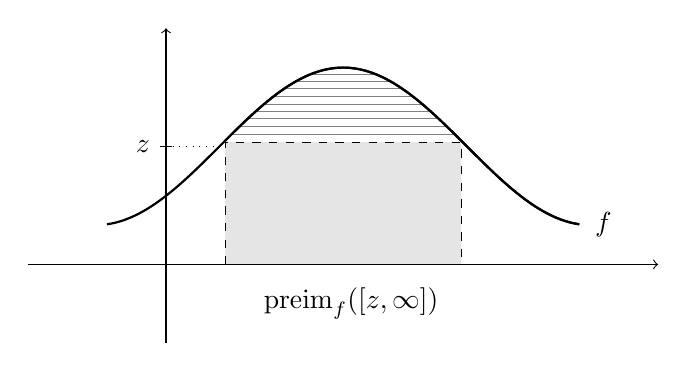
\begin{tikzpicture}
\foreach \i in {0.25,0.6,0.95,1.3,1.65,2.05,2.5,3,3.55} {
\draw[gray] (-0.5+0.3*\i,{1.5+cos deg (-0.5+0.3*\i-1)}) -- (2.5-0.3*\i,{1.5+cos deg (2.5-0.3*\i-1)}) ;
}
\fill[black!10!white] (-0.5,0) rectangle (2.5,1.55);
\draw[dashed,thin] (-0.5,0)--(-0.5,1.55)--(2.5,1.55)--(2.5,0);
\draw (-1.17,1.5)--(-1.33,1.5) node[left] {$z$};
\draw (1.1,-0.5) node {$\preim_f([z,\infty])$};
\draw[dotted] (-1.25,1.5)--(-0.5,1.5);
\draw [thick,smooth,samples=100,variable=\x,domain=-2:4] plot(\x,{1.5+cos deg (\x-1)}) node[right=2pt] {$f$};
\draw [thick,smooth,samples=100,variable=\x,domain=-0.5:4] plot(\x,{1.5+cos deg (\x-1)});
\draw[->,thin] (-3,0)--(5,0);
\draw[->,thin] (-1.25,-1)--(-1.25,3);
\end{tikzpicture}
\end{center}

The following is the pivotal theorem of Lebesgue integration.

\begin{theorem}[Monotone convergence theorem]
Let $(M,\Sigma,\mu)$ be a measure space and let $\{f_n\}_{n\in\N}$ be a sequence of non-negative, measurable functions $M\to\overline{\R}$ such that $f_{n+1}\geq f_n$ for all $n\in \N$. If there exists a function $f\cl M\to \overline{\R}$ such that
\begin{equation*}
\forall \, m \in M : \ \lim_{n\to\infty}f_n(m) = f(m)
\end{equation*}
(i.e. $f$ is the pointwise limit of  $\{f_n\}_{n\in\N}$), then $f$ is measurable and
\begin{equation*}
\lim_{n\to\infty}\int_M\! f_n \, \d \mu = \int_M\! f \, \d \mu.
\end{equation*}
\end{theorem}

\begin{remark}
Observe that this result is in stark contrast with what one may be used from Riemann integration, where pointwise converge of a sequence of integrable functions $\{f_n\}_{n\in\N}$ is \emph{not} a sufficient condition for the integral of the limit $f$ to be equal to the limit of the integrals of $f_n$ or, in fact, even for $f$ to be integrable. For these, we need stronger conditions on the sequence $\{f_n\}_{n\in\N}$, such as uniform converge.
\end{remark}

The definition of the integral as a supremum is clear and geometrically reasonable. However, it is in general very difficult to evaluate
the integral of any particular function using it. The monotone convergence theorem provides a much simpler way to evaluate the integral. One can show that, for any non-negative, measurable function $f$, there exists an increasing sequence $\{s_n\}_{n\in\N}$ of non-negative, measurable, simple functions (which can be explicitly constructed from $f$) whose pointwise limit is $f$, and hence we have
\begin{equation*}
\int_M\! f \, \d \mu = \lim_{n\to\infty}\int_M\! s_n \, \d \mu,
\end{equation*}
where the right-hand side can usually be evaluated fairly easily.

\begin{example}
Consider the measure space $(\N,\mathscr{P}(\N),\mu)$, where $\mu$ is the counting measure, and let $f\cl \N \to \overline{\R}$ be non-negative. Note that the choice of $\sigma$-algebra $\mathscr{P}(\N)$ on $\N$ makes every function on $\N$ (to any measurable space) measurable. Define, for every $n\in \N$,  
\begin{equation*}
s_n=\sum_{i=0}^nf(i)\chi_{\{i\}}.
\end{equation*}
Then, $\{s_n\}_{n\in\N}$ is an increasing sequence of non-negative, measurable, simple functions whose pointwise limit is $f$ and therefore, by the monotone convergence theorem,
\begin{equation*}
\int_{\N}\! f \,\d \mu =\lim_{n\to\infty}\int_{\N}\! s_n \, \d \mu = \lim_{n\to\infty}\sum_{i=0}^nf(i)\mu(\{i\}) = \sum_{i=0}^{\infty}f(i).
\end{equation*}
If you every wondered why series seem to share so many properties with integrals, the reason is that series are just integrals with respect to a discrete measure.
\end{example}

The monotone convergence theorem can be used to extend some of properties of integrals of non-negative, measurable simple functions to non-negative, measurable functions which are not-necessarily simple.

\begin{lemma}
Let $(M,\Sigma,\mu)$ be a measure space, let $f,g\cl M\to \overline{\R}$ be non-negative, measurable functions and let $c\in [0,\infty)$. Then
\begin{enumerate}[label=(\roman*)]
\item $\displaystyle \int_{M}\! (cf+g) \,\d \mu = c\int_{M}\! f \,\d \mu +\int_{M}\! g \,\d \mu $
\item the map $\nu_f\cl \Sigma\to [0,\infty]$ defined by $\displaystyle \nu_f(A):=\int_A\, f\, \d \mu$ is a measure on $(M,\Sigma)$
\item for any $A\in\Sigma$, we have $\displaystyle \int_{M}\!f \,\d \mu =  \int_{A}\!f \,\d \mu+ \int_{M\setminus A}\!f \,\d \mu$.
\end{enumerate}
\end{lemma}

\begin{proof}
\begin{enumerate}[label=(\roman*)]
\item Let $\{s_n\}_{n\in\N}$ and $\{t_n\}_{n\in\N}$ be increasing sequences of non-negative, measurable, simple functions whose pointwise limits are $f$ and $g$, respectively. Then, it is easy to see that $\{cs_n+t_n\}_{n\in\N}$ is an increasing sequence of non-negative, measurable, simple functions whose pointwise limit is $cf+g$. Hence, by \Cref{lem:simplelinear} and the monotone converge theorem
\begin{IEEEeqnarray*}{rCl}
\int_M\! (cf+g) \,\d \mu & = &  \lim_{n\to\infty}\int_M\! (cs_n+t_n) \, \d \mu\\
& = &  \lim_{n\to\infty}\biggl(c\int_M\! s_n \, \d \mu+\int_M\! t_n \, \d \mu\biggr)\\
& = &  c\lim_{n\to\infty}\int_M\! s_n \, \d \mu+\lim_{n\to\infty}\int_M\! t_n \, \d \mu\\
& = &  c\int_{M}\! f \,\d \mu +\int_{M}\! g \,\d \mu.
\end{IEEEeqnarray*}
\item To check that $\nu_f$ is a measure on $(M,\Sigma)$, first note that we have
\begin{equation*}
\nu_f(\varnothing) = \int_{\varnothing}\! f\, \d \mu :=\int_{M}\! f\chi_{\varnothing}\, \d \mu = 0.
\end{equation*}
Let $\{A_i\}_{i\in\N}$ be a pairwise disjoint sequence in $\Sigma$. Define, for any $n\in \N$,
\begin{equation*}
f_n:=f\chi_{\left(\bigcup_{i=0}^nA_i\right)}.
\end{equation*}
Since, for all $n\in \N$, we have $\bigcup_{i=0}^{n}A_i\subseteq\bigcup_{i=0}^{n+1}A_i$ and $f$ is non-negative, $\{f_n\}_{n\in\N}$ is an increasing sequence of non-negative, measurable, simple functions whose pointwise limits is $f\chi_{\left(\bigcup_{i=0}^{\infty}A_i\right)}$. Hence, by recalling \Cref{prp:characteristic}, we have
\begin{IEEEeqnarray*}{rCl}
\nu_f\biggl(\bigcup_{\,i=0}^{\infty}A_i\biggr) & := & \int_{\,\bigcup_{i=0}^{\infty}A_i}\! f \, \d \mu\\
& = & \int_{M} \!f\chi_{\left(\bigcup_{i=0}^{\infty}A_i\right)} \, \d \mu\\
& = & \lim_{n\to\infty}\int_{M} \!f\chi_{\left(\bigcup_{i=0}^{n}A_i\right)} \, \d \mu\\
& = & \lim_{n\to\infty}\int_{M} \biggl(f\sum_{i=0}^{n}\chi_{A_i}\biggr) \, \d \mu\\
& = & \lim_{n\to\infty}\biggl(\sum_{\,i=0}^{n}\int_{M}\! f\chi_{A_i}\, \d \mu\biggr) \\
& = & \sum_{i=0}^{\infty}\nu_f(A_i) .
\end{IEEEeqnarray*}
\item Note that $A\cap (M\setminus A)=\varnothing$. Hence, by using the fact that $\nu_f$ from part (ii) is a measure on $(M,\Sigma)$, we have
\begin{equation*}
\int_M\! f \, \d \mu  =  \nu_f(M) =  \nu_f(A)+\nu_f(M\setminus A) =  \int_A\! f\, \d \mu + \int_{M\setminus A}\! f\, \d \mu. \qedhere
\end{equation*}
\end{enumerate}
\end{proof}

Part (i) of the previous lemma and the monotone convergence theorem also imply that, for any sequence $\{f_n\}_{n\in\N}$ of non-negative, measurable functions, we have
\begin{equation*}
\int_M \biggl(\sum_{\,n=0}^{\infty}f_n \biggr) \d \mu = 
\sum_{n=0}^{\infty} \int_M \! f_n \, \d \mu.
\end{equation*}
Again, note that this result does \emph{not} hold for the Riemann integral unless stronger conditions are places on the sequence $\{f_n\}_{n\in\N}$.

Finally, we have a simple but crucial result for Lebesgue integration.

\begin{theorem}
\label{thm:aezero}
Let $(M,\Sigma,\mu)$ be a measure space and let $f\cl M\to\overline{\R}$ be a non-negative, measurable function. Then
\begin{equation*}
\int_M\! f\, \d \mu = 0 \quad \Leftrightarrow \quad f=_{\mathrm{a.e.}} 0.
\end{equation*}
\end{theorem}

\begin{proof}
\begin{itemize}
\item[$(\Rightarrow)$] Suppose that $\int_Mf\,\d\mu=0$. Define $A_n:=\{m\in M \mid f(m)>\tfrac{1}{n+1}\}$ and let
\begin{equation*}
s_n := \tfrac{1}{n+1}\chi_{A_n} .
\end{equation*}
By definition of $A_n$, we clearly have $s_n\leq f$ for all $n\in\N$. Hence,
\begin{equation*}
0\leq \int_M\!s_n\,\d\mu\leq\int_M\!f\,\d\mu=0
\end{equation*}
and thus, $\int_Ms_n\,\d\mu=0$ for all $n\in\N$. Since by definition
\begin{equation*}
\int_M\!s_n\,\d\mu = \tfrac{1}{n+1}\mu(A_n),
\end{equation*}
we must also have $\mu(A_n)=0$ for all $n\in\N$. Let $A:=\{m\in M \mid f(m)\neq 0\}$. Then, as $f$ is non-negative, we have
\begin{equation*}
A = \bigcup_{n=0}^{\infty}A_n=\bigcup_{n=0}^{\infty}\{m\in M \mid f(m)>\tfrac{1}{n+1}\}
\end{equation*}
and, since $A_n\subseteq A_{n+1}$ for all $n\in\N$, we have
\begin{equation*}
\mu(A)=\mu\biggl(\bigcup_{\,n=0}^{\infty}A_n\biggr)=\lim_{n\to\infty}\mu(A_n) = 0.
\end{equation*}
Thus, $f$ is zero except on the null set $A$. That is, $f=_{\mathrm{a.e.}}0$. 

\item[$(\Leftarrow)$] Suppose that $f=_{\mathrm{a.e.}}0$. Let $S$ be the set of non-negative, measurable, simple functions $s$ such that $s\leq f$. As $f=_{\mathrm{a.e.}}0$, we have $s=_{\mathrm{a.e.}}0$ for all $s\in S$. Thus, if
\begin{equation*}
s=\sum_{i=1}^nr_i\chi_{A_i},
\end{equation*}
we must have either $r_i=0$ or $\mu(A_i)=0$ for all $1\leq i\leq n$. Hence, for all $s\in S$,
\begin{equation*}
\int_M\! s \, \d \mu := \sum_{i=1}^nr_i\mu(A_i) =0.
\end{equation*}
Therefore, we have
\begin{equation*}
\int_M\! f \, \d \mu := \sup_{s\in S}\int_M\! s \, \d \mu  = 0.\qedhere
\end{equation*}
\end{itemize}
\end{proof}

This means that, for the purposes of Lebesgue integration, null sets can be neglected as they do not change the value of an integral. The following are some examples of this.

\begin{corollary}
Let $(M,\Sigma,\mu)$ be a measure space, let $A\in\Sigma$ and let $f,g\cl M\to\overline{\R}$ be non-negative, measurable functions. 
\begin{enumerate}[label=(\roman*)]
\item If $\mu(A)=0$, then $\displaystyle\int_A\! f \, \d \mu = 0$
\item If $f=_{\mathrm{a.e.}}g$, then $\displaystyle\int_M\! f \, \d \mu = \int_M\! g \, \d \mu$
\item If $f\leq_{\mathrm{a.e.}}g$, then $\displaystyle\int_M\! f \, \d \mu \leq \int_M\! g \, \d \mu$.
\end{enumerate}
\end{corollary}

\begin{proof}
\begin{enumerate}[label=(\roman*)]
\item Clearly, $f\chi_A =_{\mathrm{a.e.}}0$ and hence
\begin{equation*}
\int_A\! f \, \d \mu =\int_M\! f\chi_A  \, \d \mu = 0.
\end{equation*}
\item As $f=_{\mathrm{a.e.}}g$, we have $f-g=_{\mathrm{a.e.}}0$ and thus
\begin{equation*}
0 = \int_M\! (f-g) \, \d \mu =\int_M\! f \, \d \mu-\int_M\! g \, \d \mu.
\end{equation*}
\item Let $B:=\{m\in M\mid f(m)>g(m)\}$. As $f\leq_{\mathrm{a.e.}}g$, we have $\mu(B)=0$ and $f\leq g$ on $M\setminus B$. Thus
\begin{IEEEeqnarray*}{C}
\int_M\! f \, \d \mu =\int_B\! f \, \d \mu+\int_{M\setminus B}\! f \, \d \mu
 \leq  \int_{M\setminus B}\! g \, \d \mu \leq \int_M\! g \, \d \mu
\end{IEEEeqnarray*}
where we used part (i) and \Cref{lem:intineq}. \qedhere
\end{enumerate}
\end{proof}

\begin{example}
Consider $(\R,\sigma(\mathcal{O}_{\R}),\lambda)$ and let $f\cl \R \to \R$ be the \emph{Dirichlet function}
\begin{equation*}
f(r) := \begin{cases}
1 & \text{if } r\in \Q\\
0 & \text{if } r\in \R\setminus \Q.
\end{cases}
\end{equation*}
The Dirichlet function is the usual example of a function which is \emph{not} Riemann integrable (on any real interval). We will now show that we can easily assign a numerical value to its integral on any measurable subset of $\R$. First, note that a set $A\in\sigma(\mathcal{O}_{\R})$ is null with respect to the Lebesgue measure if, and only if, 
\begin{equation*}
\forall \, \varepsilon >0 : \exists \, \{I_n\}_{n\in\N} : \quad A\subset \bigcup_{n=0}^{\infty}I_n \ \text{ and } \ \sum_{n=0}^{\infty}\lambda(I_n)<\varepsilon
\end{equation*}
where $\{I_n\}_{n\in\N}$ is a sequence of real intervals. From this, it immediately follows that any countable subset of $\R$ has zero Lebesgue measure. Thus, $\lambda(\Q)=0$ and hence, $f=_{\mathrm{a.e.}}0$. Therefore, by the previous lemmas, we have
\begin{equation*}
\int_A\! f \, \d \lambda = 0
\end{equation*}
for any measurable subset $A$ of $\R$. 
\end{example}

\section{Lebesgue integrable functions}

Since the difference $\infty-\infty$ is not defined, we cannot integrate all measurable functions. There is, however, a very small extra condition (beyond measurability) that determines the class of functions to which we can extend our previous definition.

\begin{definition}
Let $(M,\Sigma,\mu)$ be a measure space and let $f\cl M\to\overline{\R}$. The function $f$ is said to be \emph{(Lebesgue) integrable}\index{integrable function} if it is measurable and
\begin{equation*}
\int_{M}\!|f|\,\d \mu < \infty.
\end{equation*}
We denote the set of all integrable functions $M\to\overline{\R}$ by $\mathscr{L}^1_{\R}(M,\Sigma,\mu)$, or simply $\mathscr{L}^1(M)$ if there is no risk of confusion.
\end{definition}

For any $f\cl M\to \overline{\R}$, we define $f^+:=\max(f,0)$ and $f^-:=\max(-f,0)$, which are measurable whenever $f$ is measurable by part (iv) of \Cref{lem:measurable}.

\begin{equation*}
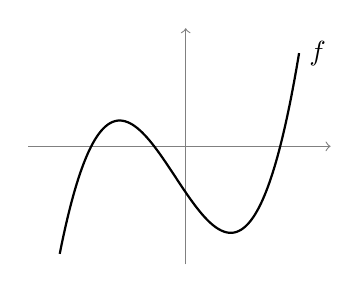
\begin{tikzpicture}[xscale=0.4,yscale=0.5]
\draw[->,thin,gray] (-5,0)--(4.6,0);
\draw[->,thin,gray] (0,-3)--(0,3);
\draw [thick,smooth,samples=100,variable=\x,domain=-4:3.6] plot(\x,{(\x+1)*(\x-3)*(\x+3)*0.13}) node[right] {$f$};
\end{tikzpicture}
\qquad\
\begin{tikzpicture}[xscale=0.4,yscale=0.5]
\draw[->,thin,gray] (-5,0)--(4.6,0);
\draw[->,thin,gray] (0,-3)--(0,3);
\draw [thick,smooth,samples=100,variable=\x,domain=-3:-1] plot(\x,{(\x+1)*(\x-3)*(\x+3)*0.13});
\draw [thick,smooth,samples=100,variable=\x,domain=3:3.6] plot(\x,{(\x+1)*(\x-3)*(\x+3)*0.13}) node[right] {$f^+$};
\draw [thick] (-4,0)--(-3,0);
\draw [thick] (-1,0)--(3,0);
\end{tikzpicture}
\qquad\
\begin{tikzpicture}[xscale=0.4,yscale=0.5]
\draw[->,thin,gray] (-5,0)--(4.6,0);
\draw[->,thin,gray] (0,-3)--(0,3);
\draw [thick,smooth,samples=100,variable=\x,domain=-4:-3] plot(\x,{-(\x+1)*(\x-3)*(\x+3)*0.13});
\draw [thick,smooth,samples=100,variable=\x,domain=-1:3] plot(\x,{-(\x+1)*(\x-3)*(\x+3)*0.13}) node[above=20pt] {$\ f^-$};
\draw [thick] (-3,0)--(-1,0);
\draw [thick] (3,0)--(3.7,0);
\end{tikzpicture}
\end{equation*}
Observe that $f=f^+-f^-$ and $|f|=f^++f^-$. Clearly, we have $f^+\leq|f|$ and $f^-\leq |f|$, and hence


\begin{equation*}
\int_{M}\!|f|\,\d \mu < \infty\quad \Leftrightarrow \quad \int_{M}\!f^+\,\d \mu < \infty\ \text{ and } \int_{M}\!f^-\,\d \mu < \infty.
\end{equation*}


\begin{definition}
Let $(M,\Sigma,\mu)$ be a measure space and let $f\cl M\to\overline{\R}$ be integrable. Then, the \emph{(Lebesgue) integral}\index{Lebesgue integral} of $f$ over $M$ with respect to $\mu$ is
\begin{equation*}
\int_{M}\!f\,\d \mu := \int_{M}\!f^+\,\d \mu -\int_{M}\!f^-\,\d \mu .
\end{equation*}
\end{definition}

It should be clear that the role of the integrability condition $\int_M |f|\, \d \mu<\infty$ is to prevent the integral of $f$ from being $\infty-\infty$, which is not defined.

In quantum mechanics, we usually deal with complex functions. The extension to the complex case of the integration theory presented thus far is straightforward.

\begin{definition}
Let $(M,\Sigma,\mu)$ be a measure space. A complex function $f\cl M\to\C$ is said to be \emph{integrable} if the real functions $\Re(f)$ and $\Im(f)$ are measurable and
\begin{equation*}
\int_{M}\!|f|\,\d \mu < \infty,
\end{equation*}
where $|f|$ denotes the complex modulus, i.e.\ $|f|^2=\Re(f)^2+\Im(f)^2$. We denote the set of all integrable complex functions by $\mathscr{L}^1_{\C}(M,\Sigma,\mu)$, or simply $\mathscr{L}^1(M)$ if there is no risk of confusion.
\end{definition}

\begin{definition}
Let $(M,\Sigma,\mu)$ be a measure space and let $f\cl M\to\C$ be integrable. We define
\begin{equation*}
\int_{M}\!f\,\d \mu := \int_{M}\!\Re(f)\,\d \mu +\mathrm{i}\int_{M}\!\Im(f)\,\d \mu .
\end{equation*}
\end{definition}

The following lemma gives the properties expected of sums and scalar
multiples of integrals. Note, however, that before we show that, say,
the integral of a sum is the sum of the integrals, it is necessary to
first show that the sum of two functions in $\mathscr{L}^1(M)$ is
again in $\mathscr{L}^1(M)$.

\begin{lemma}
\label{lem:l1vs}
Let $(M,\Sigma,\mu)$ be a measure space, let $f,g \in \mathscr{L}^1(M)$ and let $c \in \R$. Then
\begin{enumerate}[label=(\roman*)]
\item $|f| \in \mathscr{L}^1(M)$ and $ \displaystyle \biggl| \int_M \! f \, \d \mu \biggr| \leq \int_M \! | f| \, \d \mu $
\item $c f \in \mathscr{L}^1(M)$ and $ \displaystyle \int_M \! cf \, \d \mu = c \int_M \!  f \, \d \mu$
\item $f+g \in \mathscr{L}^1(M)$ and $ \displaystyle \int_M \! (f+g) \, \d \mu = \int_M \!  f \, \d \mu +  \int_M \!  g \, \d \mu$
\item $\mathscr{L}^1(M)$ is a vector space.
\end{enumerate}
\end{lemma}

\begin{proof}
\begin{enumerate}[label=(\roman*)]
\item As $\bigl| |f| \bigr|=|f|$, we have $|f| \in \mathscr{L}^1(M)$. Then, by the triangle inequality,
\begin{align*}
\left|  \int_M \! f \, \d \mu \right|
&= \left|  \int_M \! f^+ \, \d \mu -   \int_M \! f^- \, \d \mu \right|\\
& \leq \left|  \int_M \! f^+ \, \d \mu  \right| + \left| \int_M \! f^- \, \d \mu \right|\\
&=  \int_M \! f^+ \, \d \mu + \int_M \! f^- \, \d \mu \\
&=  \int_M \! (f^+ + f^-)\, \d \mu  \\
&= \int_M \!  |f| \, \d \mu.
\end{align*}
\item We have
\begin{equation*}
\int_M \!  |c f| \, \d \mu = \int_M \!  |c||f| \, \d \mu = |c|\int_M \!  | f| \, \d \mu< \infty
\end{equation*}
and hence, we have $c f \in \mathscr{L}^1(M)$.

\noindent Suppose $c \geq 0$. Then, $(c f)^+ = cf^+$ and $(c f)^- = c f^-$ and thus
\begin{align*}
  \int_M \!c f \, \d \mu
  &= \int_M \! (c f)^+ \, \d \mu -   \int_M \! (c f)^- \, \d \mu\\
  &= \int_M \! c f^+ \, \d \mu -   \int_M \! c f^- \, \d \mu\\
  &=  c\int_M \! f^+ \, \d \mu -c \int_M \! f^- \, \d \mu \\
  &=  c\int_M \! (f^+ -f^-)\, \d \mu  \\
  &= c\int_M \!  f \, \d \mu
\end{align*}
Now suppose $c = -1$. Then, $(- f)^+ = f^-$ and $(- f)^- = f^+$. Thus
\begin{align*}
  \int_M \! (-f) \, \d \mu
  &= \int_M \! (- f)^+ \, \d \mu -   \int_M \! (- f)^- \, \d \mu\\
  &= \int_M \! f^- \, \d \mu -   \int_M \!  f^+ \, \d \mu\\
  &= -\biggl( \int_M \! f^+ \, \d \mu - \int_M \! f^- \, \d \mu \biggr) \\
  &=  -\int_M \! (f^+ -f^-)\, \d \mu  \\
  &= -\int_M \!  f \, \d \mu.
\end{align*}
The case $c < 0$ follows by writing $c = (-1)(-c) $ and applying the above results.
\item By the triangle inequality, we have $|f+g| \leq | f| +| g|$ and thus
\begin{equation*}
\int_M \!  |f+g| \, \d \mu \leq \int_M \!  |f| \, \d \mu + \int_M \!  |g| \, \d \mu < \infty.
\end{equation*}
Hence, $f+g \in \mathscr{L}^1(M)$. Moreover, we have
\begin{equation*}
f+g = f^+ -f^- + g^+ -g^- = (f^++g^+)-(f^-+g^-),
\end{equation*}
where $f^++g^+$ and $f^-+g^-$ are non-negative and measurable. Note that, while $(f+g)^+\neq f^++g^+$ and $(f+g)^-\neq f^-+g^-$, one can show that $f^++g^+$ and $f^-+g^-$ give an equivalent splitting of $f+g$ to define its integral.
%with
% \begin{equation*}
% \int_M \! (f^-+g^-)\, \d \mu = \int_M \! f^- \, \d \mu + \int_M \! g^- \, \d \mu < \infty .
% \end{equation*}
Therefore
\begin{align*}
  \int_M \! (f+g) \, \d \mu
  &= \int_M \!  (f^++g^+) \, \d \mu - \int_M \! (f^-+g^-) \, \d \mu\\
  &= \int_M \!  f^+ \, \d \mu + \int_M \!  g^+ \, \d \mu - \int_M \! f^- \, \d \mu - \int_M \! g^- \, \d \mu   \\
  &=  \int_M \! (f^+ -f^-)\, \d \mu  + \int_M \! (g^+ -g^-)\, \d \mu\\
  &= \int_M \!  f \, \d \mu + \int_M \!  g \, \d \mu.
\end{align*}
\item The set of all functions from $M$ to $\overline{\R}$ is a vector space. By parts (ii) and (iii), we have that $\mathscr{L}^1(M)$ is a vector subspace of this vector space and hence, a vector space in its own right. \qedhere
\end{enumerate}
\end{proof}

Some properties of the integrals of non-negative, measurable functions easily carry over to general integrable functions.

\begin{lemma}
Let $(M,\Sigma,\mu)$ be a measure space and let $f,g \in \mathscr{L}^1(M)$. 
\begin{enumerate}[label=(\roman*)]
\item If $f=_{\mathrm{a.e.}}g$, then $\displaystyle \int_M\! f \, \d \mu = \int_M\! g \, \d \mu$
\item If $f\leq_{\mathrm{a.e.}}g$, then $\displaystyle \int_M\! f \, \d \mu \leq \int_M\! g \, \d \mu$.
\end{enumerate}
\end{lemma}

Just as the monotone convergence theorem was very important for integrals of non-negative, measurable functions, there is a similar theorem that is important for integrals of functions in $\mathscr{L}^1(X)$.

\begin{theorem}[Dominated convergence theorem]
Let $(M,\Sigma,\mu)$ be a measure space and let $\{f_n\}_{n\in\N}$ be a sequence of measurable functions which converges almost everywhere to a measurable function $f$. If there exists $g \in \mathscr{L}^1(M)$ such that $|f_n| \leq_{\mathrm{a.e.}} g$ for all $n \in \N$, then
\begin{enumerate}[label=(\roman*)]
\item $f \in \mathscr{L}^1(M)$ and $f_n \in \mathscr{L}^1(M)$ for all $n \in \N$
\item $\displaystyle \lim_{n \to \infty} \int_M \!  |f_n-f| \, \d \mu =0$
\item $\displaystyle \lim_{n \to \infty} \int_M \!  f_n \, \d \mu = \int_M \!  f \, \d \mu$.
\end{enumerate}
\end{theorem}

\begin{remark}
By ``$\{f_n\}_{n\in\N}$ converges almost everywhere to $f$'' we mean, of course, that there exists a null set $A\in\Sigma$ such that
\begin{equation*}
\forall \, m \in M\setminus A : \ \lim_{n\to\infty}f_n(m)=f(m).
\end{equation*}
\end{remark}


\section[\texorpdfstring{The function spaces $L^p(M,\Sigma,\mu)$}{The
function spaces Lp(M,Sigma,mu)}]{The function spaces $L^p(M,\Sigma,\mu)$}


While in quantum mechanics we need the theory of $L^p$ spaces only for $p=2$, it is worthwhile to develop the theory in more generality, by considering $L^p$ for all $1\leq p\leq \infty$.

\begin{definition}
Let $(M,\Sigma,\mu)$ be a measure space and let $p\in [1,\infty)$. We define
\begin{equation*}
\mathscr{L}^p_{\R}(M,\Sigma,\mu) := \biggl\{f\cl M \to \overline{\R}\ \Big| \ f \text{ is measurable and } \int_M\!|f|^p\,\d \mu < \infty\biggr\}
\end{equation*}
and, similarly,
\begin{equation*}
\mathscr{L}^p_{\C}(M,\Sigma,\mu)
:=
\biggl\{
f\cl M \to \C\
\Big|
\parbox{60mm}{\centering
\(\Re(f)\) and \(\Im(f)\) are measurable \\
and \(\int_M\!|f|^p\,\d \mu < \infty\)
}
\biggr\}.
\end{equation*}
Whenever there is no risk of confusion, we lighten the notation to just $\mathscr{L}^p$.
\end{definition}


\begin{definition}
Let $(M,\Sigma,\mu)$ be a measure space and let $f\cl M \to \overline{\R}$. The \emph{essential supremum}\index{essential supremum} of $f$ is defined as
\begin{equation*}
\esup%_M
f := \inf\{c\in\overline{\R}\mid f \leq_{\mathrm{a.e.}}c\}.
\end{equation*}
Then, $f$ is said to be \emph{almost everywhere bounded (from above)} if $\esup f < \infty$. 
\end{definition}

Alternatively, $f\cl M \to \overline{\R}$ is almost everywhere bounded if there exists a null set $A\in \Sigma$ such that $f$ restricted to $M\setminus A$ is bounded.

\begin{definition}
Let $(M,\Sigma,\mu)$ be a measure space. We define
\begin{equation*}
\mathscr{L}^{\infty}_{\R}(M,\Sigma,\mu) := \biggl\{f\cl M \to \overline{\R}\ \Big| \ f \text{ is measurable and } \esup |f| < \infty\biggr\}
\end{equation*}
and, similarly,
\begin{equation*}
\mathscr{L}^{\infty}_{\C}(M,\Sigma,\mu)
:= \biggl\{
f\cl M \to \C
\ \Big| \
\parbox{60mm}{\centering
\(\Re(f)\) and \(\Im(f)\) are measurable \\
and \(\esup |f| < \infty\)
}
\biggr\}.
\end{equation*}
Whenever there is no risk of confusion, we lighten the notation to just $\mathscr{L}^p$, for $p\in[1,\infty]$.
\end{definition}

All the $\mathscr{L}^p$ spaces become vector spaces once equipped with pointwise addition and multiplication. Let us show this is detail for $\mathscr{L}_{\C}^2$.

\begin{proposition}
Let $(M,\Sigma,\mu)$ be a measure space. Then, $\mathscr{L}_{\C}^2$ is a complex vector space.
\end{proposition}

\begin{proof}
The set of all functions $M\to\C$, often denoted $M^{\C}$, is a vector space under pointwise addition and multiplication. Hence, it suffices to show that $\mathscr{L}_{\C}^2$ is a subspace of $M^{\C}$.
\begin{enumerate}[label=(\roman*)]
\item Let $f \in \mathscr{L}_{\C}^2$ and $z\in \C$. As $|z|\in \R$, we have:
\begin{equation*}
\int_M \!  |z f|^2 \, \d \mu = |z|^2 \int_M \!  |f|^2 \, \d \mu < \infty
\end{equation*}
and hence, $z f \in \mathscr{L}_{\C}^2$.
\item Let $f,g \in \mathscr{L}_{\C}^2$. Note that
\begin{align*}
|f+g|^2 
&= (f+g)\overline{(f+g)}\\
&= (f+g)(\overline{f}+\overline{g})\\
&= f\overline{f}+f\overline{g}+g\overline{f}+g\overline{g} \\
&= |f|^2 +f\overline{g}+g\overline{f}+ |g|^2.
\end{align*}
Moreover, as
\begin{equation*}
0 \leq |f-g|^2 = |f|^2 -f\overline{g}-g\overline{f}+ |g|^2 ,
\end{equation*}
we have $f\overline{g}+g\overline{f} \leq |f|^2+ |g|^2$, and thus
\begin{equation*}
|f+g|^2 \leq 2 |f|^2+ 2|g|^2.
\end{equation*}
Therefore
\begin{equation*}
\int_M \!  |f+g|^2 \, \d \mu \leq 2\int_M \!  |f|^2 \, \d \mu + 2\int_M \!  |g|^2 \, \d \mu  < \infty ,
\end{equation*}
and hence $f+g \in \mathscr{L}_{\C}^2$.\qedhere
\end{enumerate}
\end{proof}

Ideally, we would like to turn all these $\mathscr{L}^p$ space into Banach spaces. Let us begin by equipping them with a weaker piece of extra structure.

\begin{proposition}
Let $(M,\Sigma,\mu)$ be a measure space and let $p\in[0,\infty]$. Then, the maps $\|\cdot\|_p\cl \mathscr{L}^p\to\R$ defined by
\begin{equation*}
\|f\|_p:=
\begin{cases}
\biggl(\displaystyle\int_M\! |f|^p\,\d \mu\biggr)^{\negmedspace\frac{1}{p}} & \text{ for } 1\leq p<\infty\\
\esup |f| & \text{ for }p=\infty
\end{cases}
\end{equation*}
are semi-norms on $\mathscr{L}^p$. That is, for all $z\in \C$ and $f,g\in\mathscr{L}^p$,
\begin{enumerate}[label=(\roman*)]
\item $\|f\|_p\geq 0$
\item $\|z f\|_p = |z|\|f\|_p$
\item $\|f+g\|_p\leq\|f\|_p+\|g\|_p$.
\end{enumerate}
\end{proposition}
In other words, the notion of semi-norm is a generalisation of that of norm obtained by relaxing the definiteness condition. If the measure space $(M,\Sigma,\mu)$ is such that the empty set is the only null set, then $\|\cdot\|_p$ is automatically definite and hence, a norm.

\begin{example}
Consider $(\N,\mathscr{P}(\N),\mu)$, where $\mu$ is the counting measure. Then, as $\mu(A)$ is the cardinality of $A$, the only null set is the empty set. Thus, recalling that functions on $\N$ are just sequences, the maps
\begin{equation*}
\|\{a_n\}_{n\in\N}\|_p = 
\begin{cases}
\biggl(\displaystyle\sum_{\,n=0}^{\infty} |a_n|^p\biggr)^{\negmedspace\frac{1}{p}} & \text{ for } 1\leq p<\infty\\
\sup \{|a_n| \mid n\in \N\} & \text{ for }p=\infty
\end{cases}
\end{equation*}
are norms on $\mathscr{L}^p(\N)$. In particular, note that we have $\mathscr{L}^2(\N)=\ell^2(\N)$.
\end{example}

However, in general measure spaces, we only have
\begin{equation*}
\|f\|_p = 0 \quad \Leftrightarrow \quad f =_{\mathrm{a.e.}} 0,
\end{equation*}
as we have shown in \Cref{thm:aezero} for $\mathscr{L}^1$, and it is often very easy to produce an $f\neq 0$ such that $\|f\|_p=0$. The solution to this problem is to construct new spaces from the $\mathscr{L}^p$ in which functions that are almost everywhere equal are, in fact, the same function. In other words, we need to consider the quotient space of $\mathscr{L}^p$ by the equivalence relation ``being almost everywhere equal''.

\begin{definition}
Let $M$ be a set. An \emph{equivalence relation} on $M$ is a set $\sim\ \subseteq M\times M$ such that, writing $a\sim b$ for $(a,b)\in\ \sim$, we have
\begin{enumerate}[label=(\roman*)]
\item $a\sim a$ \hfill (reflexivity)
\item $a\sim b \ \Leftrightarrow\ b\sim a$ \hfill (symmetry)
\item $(a \sim b \text{ and } b\sim c) \ \Rightarrow \ a\sim c$ \hfill (transitivity)
\end{enumerate}
for all $a,b,c\in M$. If $\sim$ is an equivalence relation on $M$, we define the \emph{equivalence class} of $m\in M$ by $[m]:=\{a\in M \mid m\sim a\}$ and the \emph{quotient set} of $M$ by $\sim$ by
\begin{equation*}
M/{\sim} := \{[m]\mid m\in M\}.
\end{equation*}
\end{definition}
It is easy to show that $M/{\sim}$ is a \emph{partition} of $M$, i.e.\
\begin{equation*}
M = \bigcup_{m\in M}[m] \qquad \text{and}\qquad [a]\cap [b]=\varnothing \text{ whenever } a\neq b.
\end{equation*}
In fact, the notions of equivalence relation on $M$ and partition of $M$ are one and the same.

\begin{lemma}
Let $(M,\Sigma,\mu)$ be a measure space and let $\sim$ be defined by
\begin{equation*}
f\sim g \quad :\Leftrightarrow \quad f=_{\mathrm{a.e.}}g.
\end{equation*}
Then, $\sim$ is an equivalence relation on $\mathscr{L}^p$.
\end{lemma}

\begin{proof}
Let $f,g,h\in\mathscr{L}^p$. Clearly, $f\sim f$ and $f\sim g \Leftrightarrow g \sim f$. Now suppose that $f\sim g$ and $g\sim h$. Then, there exist null sets $A,B\in\Sigma$ such that $f=g$ on $M\setminus A$ and $g=h$ on $M\setminus B$. Recall that $\sigma$-algebras are closed under intersections and hence, $A\cap B\in\Sigma$. Obviously, we have $f=h$ on $M\setminus (A\cap B)$ and, since
\begin{equation*}
\mu(A\cap B) \leq \mu (A\cup B) \leq \mu(A)+\mu(B) = 0,
\end{equation*}
the set $A\cap B$ is null. Thus, $f\sim h$.
\end{proof}


\begin{definition}
Let $(M,\Sigma,\mu)$ be a measure space and let $f\sim g \Leftrightarrow f=_{\mathrm{a.e.}}g $. We define
\begin{equation*}
L^p := \mathscr{L}^p/{\sim} = \{[f]\mid f\in \mathscr{L}^p\}.
\end{equation*}
\end{definition}

\begin{lemma}
Let $(M,\Sigma,\mu)$ be a measure space. Then, the maps
\begin{enumerate}[label=(\roman*)]
\item $+\cl L^p\times L^p \to L^p$ defined by $[f]+[g]:=[f+g]$
\item $\cdot\cl \C\times L^p \to L^p$ defined by $z[f]:=[zf]$
\item $\|\cdot\|_p\cl L^p \to \R$ defined by $\|[f]\|_p:=\|f\|_p$
\end{enumerate}
are well-defined. Moreover, $\|\cdot\|_p\cl L^p \to \R$ is a norm on $L^p$.
\end{lemma}

\begin{lemma}[H\"older's inequality]
Let $(M,\Sigma,\mu)$ be a measure space and let $p,q\in[1,\infty]$ be such that $\tfrac{1}{p}+\tfrac{1}{q}=1$ (where $\tfrac{1}{\infty}:=0$). Then, for all measurable functions $f,g\cl M\to \C$, we have
\begin{equation*}
\biggl|\int_M\!fg \, \d \mu \biggr| \leq \biggl(\int_M\!|f|^p \, \d \mu\biggr)^{\negmedspace \frac{1}{p}}\biggl(\int_M\!|g|^q \, \d \mu\biggr)^{\negmedspace \frac{1}{q}}.
\end{equation*}
\end{lemma}

Hence, if $[f]\in L^p$ and $[g]\in L^q$, with  $\tfrac{1}{p}+\tfrac{1}{q}=1$ , then $[fg]\in L^1$ and
\begin{equation*}
\|[fg]\|_1\leq\|[f]\|^p\|[g]\|^q.
\end{equation*}

\begin{theorem}
The spaces $L^p$ are Banach spaces for all $p\in[0,\infty]$.
\end{theorem}

We have already remarked that the case $p=2$ is special in that $L^2$ is the only $L^p$ space which can be made into a Hilbert space.

\begin{proposition}
Let $(M,\Sigma,\mu)$ be a measure space and define
\begin{IEEEeqnarray*}{rrCl}
\langle\cdot|\cdot\rangle_{L^2} \cl & L^2\times L^2 & \to & \C\\
& ([f],[g]) & \mapsto & \displaystyle \int_M\!\overline{f}g\, \d \mu.
\end{IEEEeqnarray*}
Then, $\langle\cdot|\cdot\rangle_{L^2} $ is well-defined and it is a sesqui-linear inner product on $L^2$.
\end{proposition}

\begin{proof}
First note that if $[f]\in L^2$, then $[\overline{f}]\in L^2$ and hence, by H\"older inequality, $[\overline{f}g]\in L^1$. This ensures that $\bigl\langle [f]\big|[g]\bigr\rangle_{L^2}\in \C$ for all $[f],[g]\in L^2$.

To show well-definedeness, let $f'=_{\mathrm{a.e.}}f$ and $g'=_{\mathrm{a.e.}}g$. Then, $\overline{f'}g'=_{\mathrm{a.e.}}\overline{f}g$ and thus
\begin{equation*}
\bigl\langle [f']\big|[g']\bigr\rangle_{L^2} :=  \int_M\!\overline{f'}g'\, \d \mu =  \int_M\!\overline{f}g\, \d \mu =: \bigl\langle [f]\big|[g]\bigr\rangle_{L^2} .
\end{equation*}

Now, let $[f],[g],[h]\in L^2$ and $z\in \C$. Then
\begin{enumerate}[label=(\roman*)]
\item $\displaystyle\overline{\bigl\langle [f]\big|[g]\bigr\rangle}_{L^2} = \overline{\int_M\!\overline{f}g\, \d \mu} = \int_M\!f\overline{g}\, \d \mu = \bigl\langle [g]\big|[f]\bigr\rangle_{L^2}$
\item We have
\begin{IEEEeqnarray*}{rCl}
\bigl\langle [f]\big|z[g]+[h]\bigr\rangle_{L^2} & = & \int_M\!\overline{f}(zg+h)\, \d \mu \\
& = & z\int_M\!\overline{f}g\, \d \mu+\int_M\!\overline{f}h\, \d \mu \\
& = & z\bigl\langle [f]\big|[g]\bigr\rangle_{L^2}+\bigl\langle [f]\big|[h]\bigr\rangle_{L^2}
\end{IEEEeqnarray*}
\item We have $\displaystyle\bigl\langle [f]\big|[f]\bigr\rangle_{L^2} = \int_M\!\overline{f}f\, \d \mu = \int_M\!|f|^2\, \d \mu \geq 0 $ and
\begin{equation*}
\bigl\langle [f]\big|[f]\bigr\rangle_{L^2} = 0 \quad \Leftrightarrow \quad \int_M\!|f|^2\, \d \mu = 0  \quad \Leftrightarrow \quad \|[f]\|_2 = 0.
\end{equation*}
Thus, $[f]=0:=[0]$. \qedhere
\end{enumerate}
\end{proof}

The last part of the proof also shows that $\langle\cdot | \cdot \rangle_{L^2}$ induces the norm $\|\cdot\|_2$, with respect to which $L^2$ is a Banach space. Hence, $(L^2,\langle\cdot | \cdot \rangle_{L^2})$ is a Hilbert space.

\begin{remark}
The inner product $\langle\cdot | \cdot \rangle_{L^2}$ on $L^2_{\C}(\N,\mathscr{P}(\N),\mu)$ coincides with the inner product $\langle\cdot | \cdot \rangle_{\ell^2}$ on $\ell^2(\N)$ defined in the section on separable Hilbert spaces.
\end{remark}

























  \chapter{Self-adjoint and essentially self-adjoint operators}
  
While we have already given some of the following definitions in the
introductory section on the axioms of quantum mechanics, we reproduce
them here for completeness.

\section{Adjoint operators}

If \(A\colon\Cal H\to\Cal H\) is a \emph{bounded} operator,
%then for every
%\(\psi\in \Cal H\), the operator \(f_{\psi}\circ A\cl\Cal H\to\C\),
%given by \(\alpha\mapsto\langle \psi\mid A\alpha\rangle\), is linear
%and bounded. By the Riesz representation theorem, there is
%a unique \(\eta\in\Cal H\) such that
%\begin{equation}
%  f_{\psi}\circ A = f_{\eta} \equiv \langle\eta\mid-\rangle.
%\end{equation}
%Writing \(A^*\psi\equiv\eta\), this asignment gives us a
%bounded linear operator \(A^*\in\Cal L(\Cal H,\Cal H)\).
%Indeed, for every \(\psi\in\Cal H\) we have 
%\begin{align}
%  \|A^*\psi\|
%  &= \|\eta\| \\
%  &= \|f_\eta\| \\
%  &= \|f_\psi\circ A\| \\
%  &= \sup\{|\langle \psi\mid A\alpha\rangle| : \|\alpha\|\leq 1 \}\\
%  &\leq \sup\{\|\psi\|\|A\alpha\| : \|\alpha\|\leq 1 \}\\
%  &= \|\psi\|\|A\|.
%\end{align}
%This even proves that \(\|A^*\|\leq\|A\|\).
%In other words, if \(A\colon \Cal H\to\Cal H\) is \emph{bounded},
there is a unique bounded operator \(A^*\colon\Cal H\to\Cal H\),
called the \emph{adjoint} of \(A\), such that
\begin{equation}
  \forall \psi,\alpha\in\Cal H,\
  \langle \psi\mid A\alpha\rangle
  =
  \langle A^*\psi\mid \alpha\rangle.
\end{equation}
If moreover \(A=A^*\), we say that \(A\) is self-adjoint.

For various reasons, the observables in quantum mechanics are modeled
by \emph{self-adjoint operators}.
However, most of them are \emph{not bounded}.
It turns out that not-bounded operators defined on all of
\(\Cal H\) cannot be self-adjoint so, in order to have not-bounded
self-adjoint operators, we will need to allow their domain to be
only a \emph{dense subspace} \(\Cal D_A\subseteq\Cal H\).

\begin{definition}
  An \emph{operator on \(\Cal H\)} is a
  linear map $A\cl\mathcal{D}_A\to\mathcal{H}$,
  where $\mathcal{D}_A\subseteq\Cal H$ is a subspace.
  We say \(A\) is \emph{densely defined} if \(\Cal D_A\) is dense in
  \(\Cal H\), i.e.
  \begin{equation*}
    \forall \psi\in \mathcal{H}, \
    \forall \varepsilon > 0, \
    \exists \alpha \in \mathcal{D}_A, \
    \|\alpha - \psi\|< \varepsilon
  \end{equation*}
  or, equivalently, if for every $\psi\in\mathcal{H}$ there exists a
  sequence $\{\alpha_n\}_{n\in\N}$ in $\mathcal{D}_A$ whose limit is
  $\psi$.
\end{definition}
Now we define the \emph{adjoint} of a densely defined operator
\(A\colon\Cal D_A\to\Cal H\).
Note that we do \emph{not} assume that \(A\) is bounded, so when we
fix \(\psi\in\Cal H\), the linear functional
\begin{align*}
  f_\psi\circ A \colon \Cal D_A &\to \C \\
  \alpha &\mapsto \langle \psi \mid A\alpha \rangle
\end{align*}
is not necessarily bounded. However, if it \emph{is bounded},
by the BLT theorem, (\cref{thm:BLT}), it admits a unique
bounded extension \(\Cal H\to\C\) which, by the Riesz
representation theorem (\cref{thm:riesz}), is
of the form \(f_\eta\equiv\langle\eta\mid-\rangle\) for a unique
\(\eta\in\Cal H\).
In other words, \(\eta\) is the unique element of \(\Cal H\) such that
\begin{equation}
  f_\psi\circ A = f_{\eta}|_{\Cal D_A} \colon\Cal D_A\to\C
\end{equation}
or, equivalently,
\begin{equation}
  \forall\alpha\in\Cal D_A, \
  \langle \psi\mid A\alpha\rangle
  =
  \langle \eta\mid \alpha\rangle.
\end{equation}
Conversely, if there is some \(\eta\) satisfiyng these conditions,
then \(f_\psi\circ A\) is necessarily bounded (and \(\eta\) is unique).

Thus, we define the adjoint of \(A\) in the following way.
\begin{definition}
  Let $A\cl \mathcal{D}_A\to \mathcal{H}$ be a densely defined
  operator on $\mathcal{H}$. The \emph{adjoint}\index{adjoint} of $A$
  is the operator $A^*\cl\mathcal{D}_{A^*}\to\mathcal{H}$ defined as follows.
  \begin{enumerate}[label=(\roman*)]
    \item
      The domain of \(A^*\) is the subspace of \(\Cal H\) defined as
      \begin{align}
        \mathcal{D}_{A^*}
        &=
        \{
          \psi\in\mathcal{H}
          \mid
          f_\psi\circ A\colon\Cal D_A\to\C \text{ is bounded}
        \} \\
        &=
        \{
          \psi\in\mathcal{H}
          \mid
          \exists\eta\in\Cal H, \
          f_\psi\circ A=f_\eta|_{\Cal D_A}\colon\Cal D_A\to\C
        \} \\
        &=
        \{
          \psi\in\mathcal{H}
          \mid
          \exists\eta\in\Cal H, \
          \forall\alpha\in\Cal D_A, \
          \langle \psi\mid A\alpha \rangle = \langle \eta\mid\alpha\rangle
        \}
      \end{align}
    \item
      For each \(\psi\in\Cal D_{A^*}\) we define $A^*\psi$ to be the
      element \(\eta\) corresponding to \(\psi\).
      In other words, \(A^*\psi\) is
      the unique element of \(\Cal H\) satisfying
      \begin{equation}
        f_\psi\circ A = f_{A^*\psi}|_{\Cal D_A} \colon\Cal D_A\to\C.
      \end{equation}
      i.e.
      \begin{equation}
        \forall\alpha\in\Cal D_A, \
        \langle \psi\mid A\alpha\rangle
        =
        \langle A^*\psi\mid \alpha\rangle.
      \end{equation}
  \end{enumerate}
\end{definition}

\begin{remark}
  Although \(A\) is a densely defined operator,
  its adjoint \(A^*\) is not necessarily densely defined.
\end{remark}

If $A$ and $B$ are densely defined and $\mathcal{D}_A=\mathcal{D}_B$,
then the pointwise sum $A+B$ is clearly densely defined and hence,
$(A+B)^*$ exists. However, we do \emph{not} have $(A+B)^*=A^*+B^*$ in
general, unless one of $A$ and $B$ is bounded, but we do have the
following result.
\begin{proposition}
If $A$ is densely defined, then 
\begin{equation*}
(A+z\id_{\mathcal{D}_A})^*=A^*+\overline{z}\id_{\mathcal{D}_A}
\end{equation*}
for any $z\in\C$.
\end{proposition}
The identity operator $\id_{\mathcal{D}_A}$ is usually suppressed in the notation, so that the above equation reads $(A+z)^*=A^*+\overline{z}$.

% \begin{definition}
% Let $A\cl \mathcal{D}_A\to \mathcal{H}$ be a linear operator. The \emph{kernel}\index{kernel} and \emph{range}\index{range} of $A$ are
% \begin{equation*}
% \ker (A)  :=  \{\alpha \in \mathcal{D}_A \mid A\alpha = 0\},\quad\qquad\ran (A)  :=  \{A\alpha \mid \alpha \in \mathcal{D}_A \}.
% \end{equation*}
% The range is also called \emph{image}\index{image} and $\im (A)$ and $A(\mathcal{D}_A)$ are alternative notations.
% \end{definition}
% 
% \begin{proposition}
% An operator $A\cl \mathcal{D}_A\to \mathcal{H}$ is
% \begin{enumerate}[label=(\roman*)]
% \item injective if, and only if, $\ker(A)=\{0\}$
% \item surjective if, and only if, $\ran(A)=\mathcal{H}$.
% \end{enumerate}
% \end{proposition}
% 
% \begin{definition}
% An operator $A\cl \mathcal{D}_A\to \mathcal{H}$ is
% \emph{invertible}\index{invertible operator} if there exists an
% operator $B\cl\mathcal{H}\to \mathcal{D}_A$ such that $A\circ B =
% \id_{\mathcal{H}}$ and $B\circ A = \id_{\mathcal{D}_A}$.
% \end{definition}
% 
% \begin{proposition}
% An operator $A$ is invertible if, and only if, 
% \begin{equation*}
% \ker(A)=\{0\}\quad \text{ and }\quad\, \ran(A)=\mathcal{H}.
% \end{equation*}
% \end{proposition}

\begin{proposition}
\label{prp:kerran}
Let $A$ be densely defined. Then, $\ker(A^*)=\ran(A)^{\perp}$.
\end{proposition}

\begin{proof}
  Take \(\psi\in\ker(A^*)\), so \(A^*\psi=0\).
  Hence, for all \(\alpha\in\Cal D_A\), we have
  \begin{equation}
    \langle \psi \mid A\alpha \rangle
    = \langle A^*\psi \mid\alpha \rangle
    = 0
  \end{equation}
  which means that \(\psi\in\ran(A)^\perp\).
  Conversely, if \(\psi\in\ran(A)^\perp\), then
  \begin{equation}
    \langle \psi \mid A\alpha \rangle = 0.
  \end{equation}
  Hence, the linear functional \(f_\psi\circ A\colon\Cal D_A\to\C\) is
  bounded. Iin fact it is zero) and it is represen\(A^*\psi=0\), so
  \(\psi\in\ker(A^*)\).
\end{proof}

\begin{definition}
  A densely defined operator $A\cl\mathcal{D}_A\to\mathcal{H}$ is
  \emph{self-adjoint}\index{self-adjoint operator} if $A=A^*$. That is,
  \begin{enumerate}[label=(\roman*)]
    \item $\mathcal{D}_A = \mathcal{D}_{A^*}$
    \item $\forall \, \alpha \in \mathcal{D}_A : \ A\alpha = A^*\alpha$.
  \end{enumerate}
\end{definition}

\begin{definition}
  Let $A\cl \mathcal{D}_A \to \mathcal{H}$ and $B\cl \mathcal{D}_B \to
  \mathcal{H}$ be operators. We say that $B$ is an
  \emph{extension}\index{extension} of $A$, and we write $A\subseteq
  B$, iff
  \begin{enumerate}[label=(\roman*)]
  \item $\mathcal{D}_{A}\subseteq \mathcal{D}_{B}$
  \item $\forall \, \alpha \in \mathcal{D}_{A} : \ A\alpha = B \alpha$.
  \end{enumerate}
\end{definition}

\begin{proposition}
  \label{prp:adjointreverse}
  Let $A,B$ be densely defined. If $A\subseteq B$, then $B^*\subseteq
  A^*$.
\end{proposition}

\begin{proof}
  \begin{enumerate}[label=(\roman*)]
  \item Let $\psi \in \mathcal{D}_{B^*}$.
  Then the operator
  \begin{equation}
    f_\psi\circ B\colon \Cal D_B\to\C
  \end{equation}
  is bounded.
  Restricting to \(\Cal D_A\subseteq\Cal D_B\), we see that
  \begin{equation}
    f_\psi\circ A\colon \Cal D_A\to\C
  \end{equation}
  is bounded. Hence, \(\psi\in\Cal D_{A^*}\),
  which shows that $\mathcal{D}_{B^*}\subseteq \mathcal{D}_{A^*}$.
  \item
  If \(\psi\in\Cal D_{B^*}\subseteq\Cal D_{A^*}\), then for all
  \begin{equation}
    f_\psi\circ B = f_{B^*\psi}|_{\Cal D_B} \colon\Cal D_B\to\C.
  \end{equation}
  restricting to \(\Cal D_A\), we get
  \begin{equation}
    f_\psi\circ A = f_{B^*\psi}|_{\Cal D_A} \colon\Cal D_A\to\C,
  \end{equation}
  by uniqueness of \(A^*\psi\), we have $B^*\psi = A^*\psi$.
  \end{enumerate}
\end{proof}

\begin{corollary}
  \label[corollary]{cor:selfasdjext}
  A self-adjoint operator is maximal with respect to self-adjoint extension.
\end{corollary}

\begin{proof}
  Let $A,B$ be self-adjoint and suppose that $A\subseteq B$. Then
  \begin{equation*}
  A \subseteq B = B^* \subseteq A^* = A
  \end{equation*}
  and hence, $B=A$.
\end{proof}
%In fact, self-adjoint operators are maximal even with respect to
%symmetric extension, for we would have $B\subseteq B^*$ instead of
%$B=B^*$ in the above equation.

\section{The adjoint of a symmetric operator}

\begin{definition}
A densely defined operator $A\cl\mathcal{D}_A\to\mathcal{H}$ is called \emph{symmetric}\index{symmetric operator} if
\begin{equation*}
\forall \, \alpha,\beta \in \mathcal{D}_A : \ \langle\alpha|A\beta\rangle = \langle A\alpha|\beta\rangle.
\end{equation*}
\end{definition}

\begin{remark}
Observe that any self-adjoint operator is also symmetric, but a
symmetric operator need not be self-adjoint. 

In the physics literature, the term \emph{Hermitian}\index{Hermitian
operator} is sometimes used to refer to a symmetric operator, and
sometimes used to mean a self-adjoint operator.
To prevent confusions, we will avoid the term Hermitian altogether.
\end{remark}

%\begin{remark}
%In the physics literature, symmetric operators are usually referred to
%as \emph{Hermitian}\index{Hermitian operator} operators. However, this
%notion is then confused with that of self-adjointness when physicists
%say that observables in quantum mechanics correspond to Hermitian
%operators, which is not the case. On the other hand, if one decides to
%use Hermitian as a synonym of self-adjoint, it is then not true that
%all symmetric operators are Hermitian. In order to prevent confusion,
%we will avoid the term Hermitian altogether.
%\end{remark}

\begin{proposition}
  \label{prp:symext}
  A densely defined operator $A\colon\Cal D_A\to\Cal H$ is symmetric
  if, and only if, $A\subseteq A^*$.
\end{proposition}
\begin{proof}
  Suppose \(A\) is symmetric.
  Let $\psi\in\mathcal{D}_A$ and let $\eta:=A\psi$. Then, by symmetry, we have
  \begin{equation*}
    \forall \alpha\in \mathcal{D}_A, \
    \langle\psi|A\alpha\rangle = \langle \eta|\alpha\rangle
  \end{equation*}
  and hence $\psi\in\mathcal{D}_{A^*}$. Therefore,
  $\mathcal{D}_A\subseteq \mathcal{D}_{A^*}$ and $A^*\psi:=\eta =
  A\psi$.
  
  Conversely, suppose that \(A\subseteq A^*\). Then, for every
  \(\psi,\alpha\in\Cal D_A\) we have \(\psi\in D_{A^*}\) and
  \(A^*\psi=A\psi\), so
  \begin{equation}
    \langle \psi,A\alpha\rangle
    = \langle A^*\psi,\alpha\rangle
    = \langle A\psi,\alpha\rangle
  \end{equation}
  whence \(A\) is symmetric.
\end{proof}

\begin{corollary}
  A self-adjoint operator is maximal with respect to symmetric extensions.
\end{corollary}
\begin{proof}
  Same as \cref{cor:selfasdjext}, except we have \(B\subseteq B^*\)
  instead of \(B=B^*\).
\end{proof}

\section{Closability, closure, closedness}
\label{sec:closable-closure-closed}

\begin{definition}
  An operator \(A\colon\Cal D_A\to\Cal H\) (not necessarily densely defined) is \emph{closed} if its graph
  \begin{equation}
    \Gamma_A
    = \{(\psi,A\psi) : \psi\in\Cal D_A\}
    \subseteq \Cal H\times\Cal H
  \end{equation}
  is a closed subset of \(\Cal H\times\Cal H\).
  Equivalently, \(A\) is closed if, for each sequence \(\psi_n\) in
  \(\Cal D_A\) with \(\psi_n\to\psi\in\Cal H\) and \(A\psi_n \to
  \alpha\in\Cal H\), we have \(\psi\in\Cal D_A\) and \(A\psi=\alpha\).

  The operator \(A\) is called \emph{closable} if the closure of its
  graph is the graph of an operator \(\overline A\):
  \begin{equation}
    \overline{\Gamma_A}
    = \{(\psi,\overline A\psi) : \psi\in\Cal D_{\overline A}\}
    \subseteq \Cal H\times\Cal H.
  \end{equation}
  Then \(\overline A\) is necessarily unique, it is closed and it
  extends \(A\).
\end{definition}

\begin{remark}
Note that we have used the overline notation in several contexts with
different meanings. When applied to complex numbers, it denotes
complex conjugation. When applied to subsets of a topological space,
it denotes their topological closure. Finally, when applied to
(closable) operators, it denotes their closure as defined above.
\end{remark}

\begin{proposition}
  If \(A\colon\Cal D_A\to\Cal H\) is a densely defined operator, then
  its adjoint \(A^*\) is closed.
\end{proposition}
\begin{proof}
  Suppose \(\psi_n\in\Cal D_{A^*}\) converges to \(\psi\in\Cal H\) and
  \(A^*\psi_n\) converge to \(\alpha\in\Cal H\).
  Then, for every \(\beta\in\Cal D_A\), we have
  \begin{align}
    \langle \alpha \mid \beta \rangle
    &= \lim_{n\to\infty}\langle A^*\psi_n \mid \beta \rangle \\
    &= \lim_{n\to\infty}\langle \psi_n \mid A\beta \rangle \\
    &= \langle \psi \mid A\beta \rangle.
  \end{align}
  Hence, the operators \(f_\psi\circ A\colon \Cal D_A\to\C\) and
  \(f_\alpha|_{\Cal D_A}\colon\Cal D_A\to\C\) are equal,
  which means that \(\psi\in\Cal D_{A^*}\) and \(A^*\psi=\alpha\).
\end{proof}

\begin{proposition}
  \label{lem:closableext}
  Let \(A\colon\Cal D_A\to\Cal H\) be a densely defined operator.
  \begin{enumerate}[label=(\roman*)]
    \item 
      If $A$ is closable, then \(A^*\) is densely defined.
    \item
      Conversely, if $A^*$ is densely defined,
      then \(A\subseteq A^{**}\), so \(A\) is closable and, in fact,
      $\overline{A}=A^{**}$.
  \end{enumerate}
\end{proposition}

\begin{proof}
  First we check (i).
  Suppose that \(A^*\) is densely defined.
  We begin by showing that \(\Cal D_A\) is contained in
  \begin{equation}
    \mathcal{D}_{A^{**}}=
    \{\psi\in \mathcal{H}\mid
    \exists\eta\in\Cal H,\
    \forall\alpha\in \mathcal{D}_{A^*}, \
    \langle \psi | A^*\alpha \rangle=\langle \eta | \alpha \rangle
    \}
  \end{equation}
  Take \(\psi\in \Cal D_A\). By definition of \(A^*\),
  \begin{equation*}
    \forall \alpha \in\mathcal{D}_{A^*}, \
    \langle \alpha | A\psi \rangle =  \langle A^* \alpha | \psi \rangle.
  \end{equation*}
  Taking complex conjugates, we obtain
  \begin{equation*}
    \forall \alpha \in\mathcal{D}_{A^*}, \
    \langle \psi | A^* \alpha \rangle
    = 
    \langle A\psi | \alpha \rangle,
  \end{equation*}
  so \(\psi\in\Cal D_{A^{**}}\).
  This also shows that $A^{**}\psi= A\psi$, so $A\subseteq A^{**}$, as
  we wanted. To show that \(A^{**}=\overline{A}\),
  take anoter closed extension \(B\) of \(A\).
  Since \(A\subseteq B\), then \(B\) is necessarily densely defined,
  so applying \cref{prp:adjointreverse} we obtain
  \(B^*\subseteq A^*\).
  twice, we see that
  \(A^{**}\subseteq B^{**}=B\), as we wanted.
  \end{proof}
  
  \begin{proposition}
  Let \(A\) be a symmetric operator. Then
  \begin{enumerate}[label=(\roman*)]
    \item \(A\) is closable,
    \item \(A^{**}\subseteq A^*\), so \(A\subseteq A^{**}\subseteq A^*\),
    \item \(A^{**}\) is symmetric.
  \end{enumerate}
  \end{proposition}
\begin{proof}
  By definition, a symmetric operator \(A\) is densely defined.
  Moreover, in \cref{prp:symext}, we saw that $A\subseteq A^*$.
  In particular, $\mathcal{D}_A\subseteq \mathcal{D}_{A^*}$, so
  \begin{equation*}
    \mathcal{H}
    =\overline{\mathcal{D}_A}\subseteq \overline{\mathcal{D}_{A^*}}.
  \end{equation*}
  Hence, $\overline{\mathcal{D}_{A^*}} = \mathcal{H}$, so \(A\) is
  closable. 
  For (ii), note that, since $A$ is symmetric, we have
  $A\subseteq A^*$ by \cref{prp:symext}.
  Hence, $A^{**}\subseteq A^*$ by \cref{prp:adjointreverse}.
  Finally, for (iii), take \(\alpha,\psi\in\Cal D_{A^{**}}\).
  By part (ii), we have \(\psi\in\Cal D\) and \(A^{**}\psi=A^*\psi\),
  so
  \begin{equation}
    \langle A^{**}\alpha\mid\psi\rangle
    = \overline{\langle A^*\psi\mid\alpha\rangle}
    = \langle \alpha\mid A^{**}\psi\rangle
  \end{equation}
\end{proof}

Note that the adjoint of a symmetric operator need
\emph{not} be symmetric.

% What?
\begin{theorem}
Let $A$ be a densely defined operator.
\begin{enumerate}[label=(\roman*)]
\item If $A$ is invertible, we have $(A^{-1})^*=(A^*)^{-1}$
\item If $A$ is invertible and closable and $\overline{A}$ is injective, then $\overline{A^{-1}}=\overline{A}^{\,-1}$.
\end{enumerate}
\end{theorem}

\section{Essentially self-adjoint operators}

Usually, checking that an operator is symmetric is easy. By contrast, checking that an operator is self-adjoint (directly from the definition) requires the construction of the adjoint, which is not always easy. However, since every self-adjoint operator is symmetric, we can first check the symmetry property, and then determine criteria for when a symmetric operator is self-adjoint, or for when a self-adjoint extension exists.

Two complications with the extension approach are that, given a symmetric operator, there could be \emph{no} self-adjoint extension at all, or there may be \emph{several} different self-adjoint extensions. There is, however, a class of operators for which the situation is much nicer.

\begin{definition}
A symmetric operator $A$ is called \emph{essentially self-adjoint}\index{essentially self-adjoint operator} if $\overline{A}$ is self-adjoint.
\end{definition}

This is weaker than the self-adjointness condition.

\begin{proposition}
If $A$ is self-adjoint, then it is essentially self-adjoint. 
\end{proposition}

\begin{proof}
If $A = A^*$, then $A\subseteq A^*$ and $A^* \subseteq A$. Hence, $A^{**}\subseteq A^*$ and $A^*\subseteq A^{**}$, so $A^* = A^{**}$. Similarly, we have $A^{**} = A^{***}$, which is just $\overline{A}=\overline{A}^{\,*}$.
\end{proof}

\begin{theorem}
If $A$ is essentially self-adjoint, then there exists a unique self-adjoint extension of $A$, namely $\overline{A}$.
\end{theorem}

\begin{proof}
\begin{enumerate}[label=(\roman*)]
\item Since $A$ is symmetric, it is closable and hence $\overline{A}$ exists.
\item By \Cref{lem:closableext}, we have $A\subseteq \overline{A}$, so $\overline{A}$ is an extension of $A$. 
\item Suppose that $B$ is another self-adjoint extension of $A$. Then, $A\subseteq B = B^*$, hence $B^{**}\subseteq A^*$, and thus $A^{**}\subseteq B^{***}=B$. This means that $\overline{A}\subseteq B$, i.e.\ $B$ is a self-adjoint extension of the self-adjoint operator $\overline{A}$. Hence, $B=\overline{A}$ by \Cref{cor:selfasdjext}.\qedhere
\end{enumerate}
\end{proof}

\begin{remark}
One may get the feeling at this point that checking for essential self-adjointness of an operator $A$, i.e.\ checking that $A^{**}=A^{***}$, is hardly easier than checking whether $A$ is self-adjoint, that is, whether $A=A^*$. However, this is not so. While we will show below that there is a sufficient criterion for self-adjointness which does not require to calculate the adjoint, we will see that there is, in fact, a necessary and sufficient criterion to check for essential self-adjointness of an operator without calculating a single adjoint.
\end{remark}

\begin{remark}
If a symmetric operator $A$ fails to even be essentially self-adjoint, then there is either no self-adjoint extension of $A$ or there are several. 
\end{remark}

\begin{definition}
Let $A$ be a densely defined operator. The \emph{defect indices}\index{defect indices} of $A$ are
\begin{equation*}
d_+:=\dim (\ker(A^*-\mathrm{i})) , \qquad \quad d_- :=\dim (\ker (A^*+\mathrm{i})),
\end{equation*}
where by $A^*\pm\mathrm{i}$ we mean, of course, $A^*\pm\mathrm{i}\cdot\id_{\mathcal{D}_A}$.
\end{definition}

\begin{theorem}
A symmetric operator has a self-adjoint extension if its defect indices coincide. Otherwise, there exist no self-adjoint extension.
\end{theorem}

\begin{remark}
We will later see that if $d_+=d_-=0$, then $A$ is essentially self-adjoint.
\end{remark}

\section{\texorpdfstring
  {Criteria for self-adjointness \\ and essential self-adjointness}
  {Criteria for self-adjointness and essential self-adjointness}
}

\begin{theorem}
A symmetric operator $A$ is self-adjoint if (but not only if)
\begin{equation*}
\exists \, z\in\C :\ \ran(A+z)=\mathcal{H}=\ran(A+\overline{z}).
\end{equation*}
\end{theorem}

\begin{proof}
Since $A$ is symmetric, by \Cref{prp:symext}, we have $A\subseteq A^*$. Hence, it remains to be shown that $A^*\subseteq A$. To that end, let $\psi\in \mathcal{D}_{A^*}$ and let $z\in \C$. Clearly, 
\begin{equation*}
A^*\psi+\overline{z}\psi\in\mathcal{H}.
\end{equation*}
Now suppose that $z$ satisfies the hypothesis of the theorem. Then, as $\ran(A+\overline{z})=\mathcal{H}$,
\begin{equation*}
\exists \, \alpha\in\mathcal{D}_{A} : \ A^*\psi+\overline{z}\psi = (A+\overline{z})\alpha.
\end{equation*}
By using the symmetry of $A$, we have that, for any $\beta\in\mathcal{D}_A$,
\begin{IEEEeqnarray*}{rCl}
\langle \psi| (A+z)\beta \rangle & = & \langle (A+z)^*\psi| \beta \rangle \\
 & = & \langle A^*\psi+\overline{z}\psi| \beta \rangle \\
 & = & \langle (A+\overline{z})\alpha | \beta \rangle  \\
 & = & \langle A\alpha | \beta \rangle +z\langle \alpha | \beta \rangle \\
 & = & \langle \alpha | A\beta \rangle +\langle \alpha | z\beta \rangle \\
 & = & \langle \alpha | (A+z)\beta \rangle.
\end{IEEEeqnarray*}
Since $\beta\in\mathcal{D}_A$ was arbitrary and $\ran(A+z)=\mathcal{H}$, we have
\begin{equation*}
\forall \, \varphi \in \mathcal{H} : \quad \langle \psi | \varphi\rangle= \langle \alpha | \varphi \rangle.
\end{equation*}
Hence, by positive-definiteness of the inner product, we have $\psi\in\alpha$, thus $\psi\in\mathcal{D}_A$ and therefore, $A^*\subseteq A$.
\end{proof}


\begin{theorem}
A symmetric operator $A$ is essentially self-adjoint if, and only if, 
\begin{equation*}
\exists \, z\in \C\setminus \R : \ \overline{\ran(A+z)}=\mathcal{H}=\overline{\ran(A+\overline{z})}. 
\end{equation*}
\end{theorem}

The following criterion for essential self-adjointness, which does require the calculation of $A^*$, is equivalent to the previous result and, in some situations, it can be easier to check.

\begin{theorem}
A symmetric operator $A$ is essentially self-adjoint if, and only if,
\begin{equation*}
\exists \, z\in \C\setminus \R : \ \ker(A^*+z)=\{0\}=\ker(A^*+\overline{z}). 
\end{equation*}
\end{theorem}

\begin{proof}
We show that this is equivalent to the previous condition. Recall that if $\mathcal{M}$ is a linear subspace of $\mathcal{H}$, then $\mathcal{M}^{\perp}$ is closed and hence, $\mathcal{M}^{\perp\perp}=\overline{M}$. Thus, by \Cref{prp:kerran}, we have
\begin{equation*}
\overline{\ran(A+z)}  =  \ran(A+z)^{\perp\perp}
 =  \ker(A^*+\overline{z})^{\perp}
\end{equation*}
and, similarly,
\begin{equation*}
\overline{\ran(A+z)} = \ker(A^*+z).
\end{equation*}
Since $\mathcal{H}^{\perp}=\{0\}$, the above condition is equivalent to
\begin{equation*}
\overline{\ran(A+z)}=\mathcal{H}=\overline{\ran(A+\overline{z})}.\qedhere
\end{equation*}
\end{proof}























  \chapter{Spectra and perturbation theory}
  \input{08spectra}

  \chapter{Case study: momentum operator}
  
We will examine an example of an operator which will put our machinery
to work.

Our operator will be the \emph{momentum} operator
\begin{align}
  P_j \colon \Cal D_P &\to L^{2}(\R^{d}) \\
  \psi & \mapsto -\ic\hbar \partial_j\psi
\end{align}
For the purpose of showing the basic principles of the theory,
it is enough to take \(d=1\).

The first problem we must address is to choose the domain \(\Cal
D_P\). Of course, it cannot be the whole space \(L^{2}(\R)\).
Often, one is just ``given the operator'' without a domain, but really
one needs the domain to know whether the operator \(P\) is
self-adjoint. In fact, we want to pick a domain \(\Cal D_P\) such
that \(P\) \emph{is} self-adjoint, since it is supposed to be an
observable of a physical system.

In fact, instead of the real line \(\R\), we will first look at the
problem on a closed interval \([0,1]\), by choosing the domain to be
\begin{equation}
  \Cal D_P = \{\psi\in C^{1}[0,1] \mid \psi(0)=\psi(1)=0\}
,\end{equation}
where it will turns out that the operator cannot be made self-adjoint
in a unique way.
Then we will look at the same problem over the circle, by choosing the
domain
\begin{equation}
  \Cal D_P = \{\psi\in C^{1}[0,1] \mid \psi(0)=\psi(1)\}
,\end{equation}
where the momentum operator it will turn out to be essentially
self-adjoint, so it will have a unique self-adjoint extension.
In both cases, the Hilbert space under consideration will be \(\Cal
H=L^{2}[0,1]\).

\section{Absolutely continuous functions and Sobolev spaces}

We will encounter the spaces
\begin{equation}
  C^{1}[a,b] \subseteq H^{1}[a,b] \subseteq \AC[a,b]
.\end{equation}

\begin{definition}
  A function \(\psi\colon[a,b]\to\C\) is called \emph{absolutely
  continuous} if there is an integrable function
  \(\rho\colon[a,b]\to\C\) such that
  \begin{equation}
    \label{eq:abscont}
    \psi(x) = \psi(a) + \int_{a}^{x}\rho(y)\d y
  .\end{equation}
  The subspace of the elements \(\psi\in L^{2}[a,b]\) with an absolutely
  continuous representative is denoted \(\AC[a,b]\).
\end{definition}

Recall that integrable functions on \([a,b]\) are just \(L^{1}[a,b]\)
(after identifying almost-everywhere equal functions).

Note that, if \(\psi\in L^{1}[a,b]\) has an absolutely continuous
representative, then the integrable function \(\rho\) in equation
\eqref{eq:abscont} is unique up to almost-everywhere equality.
Hence, we have a differentiation map
\begin{equation}
  D \colon \AC[a,b]\to L^{1}[a,b]
\end{equation}
taking \(\psi\mapsto\rho\). We write \(\psi'=\rho\).

\begin{definition}
  The subspace \(H^{1}[a,b]\) of all \(\psi\in\AC[a,b]\) such that
  \(\psi'\in L^{2}[a,b]\) is called the \(1\)-th Sobolev space.
\end{definition}

\section{Momentum operator on a compact interval}

Consider the operator
\begin{align}
  P \colon \Cal D_P &\to L^{2}(\R^{d}) \\
  \psi & \mapsto -\ic \psi'
\end{align}
with domain
\begin{equation}
  \Cal D_P = \{\psi\in C^{1}[0,1] \mid \psi(0)=\psi(1)=0\}
.\end{equation}

The main question we want to tackle is:
\emph{is this operator self-adjoint?}

To even have a possibility of being self adjoint, it must be
symmetric. This is easier to check:
Take \(\psi,\phi\in\Cal D_P\). Using integration by parts, we have
\begin{align}
  \langle \psi,P\phi\rangle
  &= \int_{0}^{1} dx\ \bar\psi(x) (-\ic) \phi'(x) \\
  &= - \int_{0}^{1} dx \ \bar\psi'(x) (-\ic) \phi(x)
  + \cancelto{0}{\bar\psi(x)\phi(x) |_0^{1}} \label{eq:cancellation}\\
  &= \int_{0}^{1} dx \ \bar\psi'(x) \ic \phi(x) \\
  &= \int_{0}^{1} dx \ \overline{-\ic\psi'(x)} \phi(x) \\
  &= \langle P\psi,\phi\rangle
,\end{align}
so \(P\) is, indeed, symmetric.
We now calculate the adjoint \(P^{*}\).

\subsection{Calculating the adjoint on the interval}
Since \(P\) is symmetric, we know (\cref{prp:symext})
that \(P\subseteq P^{*}\), so \(P\) is self-adjoint iff the inclusion
\(\Cal D_P\subseteq \Cal D_{P^{*}}\) is an equality.
So, let's calculate the domain of \(P^*\).
An element \(\psi\in L^{2}[0,1]\) is in \(\Cal D_{P^{*}}\) iff
\begin{equation}
  \exists\eta\in L^{2}[0,1], \
  \forall\phi\in \Cal D_P, \
  \langle \psi, P\phi\rangle
  =
  \langle \eta, \phi\rangle,
\end{equation}
i.e.
\begin{equation}
  \exists\eta\in L^{2}[0,1], \
  \forall\phi\in \Cal D_P, \
  \int_{0}^{1}dx\, \bar\psi(x) (-\ic)\phi'(x)
  =
  \int_{0}^{1}dx\, \bar\eta(x) \phi(x).
\end{equation}
Now, every \(\eta\in L^{2}[0,1]\) is also integrable
(from measure theory),
so the function
\begin{equation}
  N(x) = \int_{0}^{x}\eta(x)\,dx
\end{equation}
is absolutely continuous with \(N'=\eta\). Hence,
\begin{align}
  \int_{0}^{1}dx\, \bar\eta(x) \phi(x)
  &= \int_{0}^{1}dx\, \bar N'(x) \phi(x) \\
  &= -\int_{0}^{1}dx\, \bar N(x) \phi'(x)
    + \cancelto{0}{\bar N(x)\phi(x)}
\end{align}
Hence, \(\psi\in L^{2}[0,1]\) is in \(\Cal D_{P^*}\) iff
\begin{equation}
  \exists N\in \AC[0,1], \
  \forall\phi\in \Cal D_P, \
  \int_{0}^{1}dx\, \bar\psi(x) (-\ic)\phi'(x)
  =
  -\int_{0}^{1}dx\, \bar N(x) \phi(x).
\end{equation}
i.e., iff
\begin{equation}
  \exists N\in \AC[0,1], \
  \forall\phi\in \Cal D_P, \
  \int_{0}^{1}dx\, \overline{(N(x)+\ic\psi(x))} \phi'(x)
  =0
\end{equation}
This condition means that there is an absolutely continuous
\(N\colon[0,1]\to\C\) such that \(N+\ic\psi \in \{\phi' \mid
\phi\in\Cal D_P\}^{\perp}=D(\Cal D_P)^{\perp}\).
Note that
\begin{equation}
  D(\Cal D_P) = \{f\in C^{0}[0,1] : \textstyle\int_{0}^{1}f(x)\d x=0\}
\end{equation}
and
\begin{equation}
  \overline{D(\Cal D_P)}
  = \{1\}^{\perp}
,\end{equation}
so \(D(\Cal D_P)^{\perp} = \langle 1\rangle\) are the constant
functions.
Hence, \(\psi\in\Cal D_{P^*}\) iff there is \(N\in\AC[0,1]\) such that
\(N+\ic\psi = c\) is a constant, but this happens iff \(\psi\in\AC[0,1]\).
Since we want \(P\psi=(-\ic)\psi'\in L^{2}[0,1]\), we conclude that
\(\Cal D_{P^*}=H^{1}[0,1]\).
We also know that the action of \(P^*\) is given by
\(P^{*}\psi=\eta=N'=(c-\ic\psi)'=-\ic\psi'\). In short, we calculated
that the adjoint of \(P\) is
\begin{align}
  P^{*}\colon H^{1}[0,1] &\to L^{2}[0,1] \\
  \psi &\mapsto -\ic\psi'
.\end{align}
Note that, as expected, \(\Cal D_P\subseteq \Cal D_{P^*}\), but this
inclusion is \emph{not} an equality, so \(P\) is \emph{not}
self-adjoint.

What hope do we have?
There is still the posibility that \(P\) is \emph{essentially self
adjoint}, i.e. that the closure \(P^{**}\) is self adjoint. This would
be the next best case, since that would mean that \(P^{**}\) is the
\emph{unique} self-adjoint extension of \(P\).

\subsection{Calculating the closure on the interval}

Recall that \(P\) is symmetric.
In this case we have
\begin{equation}
  P\subseteq P^{**}\subseteq P^{*}
\end{equation}
and we know that \(P^{**}\) is symmetric.
Note that the adjoint of \(P^{**}\) is \(P^{***}=P^{*}\)
(since \(P^{*}\) is already closed).
Hence, \(P^{**}\) is self adjoint iff the inclusion \(\Cal
D_{P^{**}}\subseteq \Cal D_{P^*}\) is an equality.
We now calculate the domain of \(P^{**}\).
An element \(\psi\in \Cal D_{P^*}=H^{1}[0,1]\) is in \(\Cal
D_{P^{**}}\) iff
\begin{equation}
  \exists\eta\in L^{2}[0,1], \
  \forall\phi\in\Cal D_{P^*}, \
  \langle \psi, P^{*}\phi \rangle
  =
  \langle \eta, \phi\rangle
.\end{equation}
Given such an element \(\psi\in\Cal D_{P^{**}}\), we have \(P^{**}\psi=\eta\).
Moreover, since \(P^{**}\subseteq P^*\), we also have
\(\eta=P^{**}\psi=P^*\psi\), so we obtain
\begin{equation}
  \forall\phi\in\Cal D_{P^*}, \
  \langle \psi, P^{*}\phi \rangle
  =
  \langle P^{*}\psi, \phi\rangle
.\end{equation}
In other words, if \(\psi\in\Cal D_{P^*}=H^{1}[0,1]\) is in \(\Cal
D_{P^{**}}\), then
\begin{equation}
  \forall\phi\in H^{1}[0,1], \
  \int_{0}^{1} dx\, \bar\psi(x)(-\ic)\phi'(x)
  =
  \int_{0}^{1} dx\, \overline{(-\ic)\psi'(x)}\phi(x)
.\end{equation}
Using integration by parts and rearranging, we see that both sides
differ by a boundary term, so this is equivalent to
\begin{equation}
  \forall\phi\in H^{1}[0,1], \
  \bar\psi(x)\phi(x)|_{0}^{1} = 0
\end{equation}
which happens iff \(\psi(0)=\psi(1)=0\).
Conversely, if \(\psi\in H^{1}[0,1]\) satisfies \(\psi(0)=\psi(1)=0\),
then \(\eta=-\ic\psi'\in L^{2}[0,1]\) satisfies, for all \(\phi\in
H^{1}[0,1]\)
\begin{align}
  \langle \psi, P^{*}\phi \rangle
  &= \int_{0}^{1} \bar\psi(x)(-\ic)\phi'(x)\d x \\
  &= -\int_{0}^{1} \bar\psi'(x)(-\ic)\phi(x)\d x
  + (-\ic)\bar\psi(x)\phi(x)|_{0}^{1} \\
  &= -\int_{0}^{1} \bar\psi'(x)(-\ic)\phi(x)\d x
  + (-\ic)\cancelto{0}{\bar\psi(x)\phi(x)|_{0}^{1}} \\
  &= \int_{0}^{1} \bar\psi'(x)\ic\phi(x)\d x \\
  &= \int_{0}^{1} \overline{-\ic\psi'(x)}\phi(x)\d x \\
  &= \langle \eta,\phi\rangle
,\end{align}
so \(\phi\in\Cal D_{P^{**}}\).
We conclude that
\begin{equation}
  \label{eq:domainpss}
  \Cal D_{P^{**}} = \{\psi\in H^{1}[0,1] : \psi(0)=\psi(1)=0\}
.\end{equation}
In particular, the inclusion \(\Cal D_{P^{**}}\subseteq \Cal
D_{P^*}\) is \emph{not} an equality.
(Note that, to reach this conclusion, we only
actually needed the inclusion \(\subseteq\) in equation
\eqref{eq:domainpss}, but we checked the other inclusion for fun).
Thus, we have shown that \(P^{**}\) is \emph{not} self adjoint, which
means that \(P\) is not even \emph{essentially} self-adjoint.

The situation looks bad.
Since \(P\) is not essentially self-adjoint, we cannot conclude that
it has a unique self-adjoint extension. However, it may be worse: it
could have no self-adjoint extension at all. To check for this
possibility, we calculate its defect indices.

\subsection{Calculating defect indices on the interval}

Recall that if an operator \(A\) has equal defect indices
\begin{equation}
  d_+ = \dim \ker(P^{*}-\ic),
  \qquad
  \qquad
  d_- = \dim \ker(P^{*}+\ic)
,\end{equation}
then \(A\) has a self-adjoint extension.
We calculate the kernels on the right hand sides, so we need to
determine the space of the \(\psi\in\Cal D_{P^*}=H^{1}[0,1]\) satisfying
\((P^*\mp\ic)\psi=0\), i.e. \(-\ic\psi'\mp\ic\psi=0\) or,
equivalently, \(\psi'\pm\psi=0\).
The solutions are all of the form \(\psi(x)=ae^{\mp x}\), so the
dimension of each kernel is \(1\). In particular, the defect indices
are equal, so there \emph{are} self-adjoint extensions of our operator \(P\).

In fact, it turns out that \(P\) has a family of self-adjoint
extensions, parametrized by \(U(1)\), but we won't determine it here.
Our current techniques are not enough.
We would need to learn about Cayley transforms.

An example where the operator \(P\) has \emph{no} self-adjoint
extensions is if we tried to do it on \([0,\infty)\) instead of
\([0,1]\). This means that, on a half line, there is no well-defined
momentum operator.

\section{Momentum operator on a circle}

Now we consider the operator
\begin{align}
  P \colon \Cal D_P &\to L^{2}[0,1] \\
  \psi &\mapsto -\ic\psi'
,\end{align}
where the domain is
\begin{equation}
  \Cal D_P = \{\psi\in C^{1}[0,1] \mid \psi(0)=\psi(1)\},
\end{equation}
without the condition that \(\psi\) attains the value \(0\) at the
boundary. Hence, this \(P\) is a proper extension
\begin{equation}
  \label{eq:extintcirc}
  P_{\text{interval}}
  \subsetneq
  P_{\text{circle}} = P
.\end{equation}

Again, we can check that \(P\) is symmetric. The calculation is the
same as for the interval, except that in step \eqref{eq:cancellation},
the boundary term \(\bar\psi(x)\phi(x)|_0^{1}\) vanishes for a
different reason: while for the interval every term was zero,
for the circle we only have \(\bar\psi(1)\psi(1)=\bar\psi(0)\phi(0)\).

\subsection{Calculating the adjoint on the circle}

Since \(P\) is symmetric, we know that \(P\subseteq P^{*}\).
Moreover, by equation \eqref{eq:extintcirc} it follows that
\(P^{*}\subseteq P^{*}_\text{interval}\). In particular, \(\Cal
D_{P^{*}}\subseteq H^{1}[0,1]\) and \(P^*\)
acts by \(P^*\psi=-\ic\psi'\).
Hence, taking \(\psi\in\Cal D_{P^{*}}\), we have
\begin{equation}
  \forall\phi\in\Cal D_P, \
  \langle P^*\psi, \phi \rangle
  =
  \langle \psi, P\phi \rangle
,\end{equation}
i.e.
\begin{equation}
  \forall\phi\in\Cal D_P, \
  \int_{0}^{1}dx\, \overline{-\ic\psi'(x)}\phi(x)
  =
  \int_{0}^{1}dx\, \overline{\psi(x)}(-\ic)\phi'(x)
.\end{equation}
Again, integrating by parts we see that both sides differ by a
boundary term \(\ic\bar\psi(x)\phi(x)|_{0}^{1}\), so their equality is
equivalent to the vanishing of the boundary term:
\begin{align}
  \forall\phi\in\Cal D_P, \
  \ic\bar\psi(x)\phi(x)|_{0}^{1} = 0
,\end{align}
and this happens iff \(\psi(0)=\psi(1)\).
Conversely, if \(\psi(0)=\psi(1)\), the element \(\eta=-\ic\psi'\)
satisfies the condition to be \(P^{*}\psi\), so \(\psi\in\Cal
D_{P^{*}}\).
Hence,
\begin{equation}
  \Cal D_{P^*} = \{\psi\in H^{1}[0,1] : \psi(0)=\psi(1)\}
.\end{equation}

In particular, the inclusion \(\Cal D_P\subseteq \Cal D_{P^{*}}\) is
not an equality, so \(P\) is \emph{not} self-adjoint.
Is it essentially self adjoint?

\subsection{Calculating the closure on the circle}

If \(P\) were essentially self-adjoint (i.e. if its closure \(P^{**}\)
were self-adjoint), then we would be done, since \(P^{**}\) would be
the unique self-adjoint extension of \(P\).
Again, since \(P^*\) is closed, the adjoint of \(P^{**}\) is
\(P^{***}=P^{*}\), so in view of the extensions
\begin{equation}
  P\subseteq P^{**} \subseteq P^*
\end{equation}
(which we have because \(P\) is symmetric),
it suffices to see whether the inclusion \(\Cal D_{P^{**}}\subseteq
\Cal D_{P^*}\) is an equality.
Given \(\psi\in\Cal D_{P^*}\) (i.e. \(\psi\in H^{1}[0,1]\) and
\(\psi(0)=\psi(1)\)), the function \(\eta=-\ic\psi'\in L^{2}[0,1]\)
satisfies,
\begin{align}
  \forall\phi\in\Cal D_{P^*}, \
  \langle \eta,\phi\rangle
  &= \int_{0}^{1}dx\, \overline{(-\ic)\psi'(x)}\phi(x) \\
  &= \ic\int_{0}^{1}dx\, \bar\psi'(x)\phi(x) \\
  &= -\ic\int_{0}^{1}dx\, \bar\psi(x)\phi'(x)
    + \cancelto{0}{\ic\bar\psi(x)\phi(x)|_{0}^{1}} \\
  &= \int_{0}^{1}dx\, \bar\psi(x)(-\ic)\phi'(x) \\
  &= \langle \psi,P^*\phi\rangle
,\end{align}
so \(\psi\in\Cal D_{P^{**}}\). This means that \(P^{**}=P^*\) so,
indeed, \(P^{**}\) is self-adjoint. It follows that it is the unique
self-adjoint extension of \(P\), and we are done!
Hence, the momentum operator on the circle is given by
\begin{align}
  \bar P \colon \{\psi\in H^1[0,1] : \psi(0)=\psi(1)\} &\to L^{2}[0,1]
  \\
  \psi &\mapsto -\ic\psi'
.\end{align}







  \chapter{Inverse spectral theorem}
  
This section devoted to the development of all the notions and results necessary to understand and prove the spectral theorem, stated below. 

\begin{theorem}[Spectral theorem]
For every self-adjoint operator $A\cl \mathcal{D}_A\to \mathcal{H}$ there is a unique projection-valued measure $\mathrm{P}_{\negmedspace A}\cl \sigma(\mathcal{O}_{\R})\to\mathcal{L}(\mathcal{H})$ such that
\begin{equation*}
A = \int_{\R}\! i_{\R} \, \d \mathrm{P}_{\negmedspace A} \equiv \int_{\R}\! \lambda \, \mathrm{P}_{\negmedspace A}(\d \lambda),
\end{equation*}
where $i_{\R}\cl \R\hookrightarrow \C$ is the inclusion of $\R$ into $\C$.
\end{theorem}

While useful in theory, existence results are often of limited use in practice since they usually only tell us that something exists, and not how to construct it. However, we should note here that the proof of the spectral theorem is, in fact, constructive in nature. Hence, given any self-adjoint operator $A$, we will be able to explicitly determine its associated projection-valued measure $\mathrm{P}_{\negmedspace A}$ along the following steps.
\begin{enumerate}[label=(\roman*)]
  \item For each $\psi\in\mathcal{H}$, construct the real-valued Borel measure $\mu^A_{\psi}\cl \sigma(\mathcal{O}_{\R})\to \R$ given by
  \begin{equation*}
  \mu^A_{\psi} ((-\infty,\lambda]):= \lim_{\delta\to 0^+} \lim_{\varepsilon\to 0^+} \int_{-\infty}^{\lambda+\delta}\!\d t  \Im\langle\psi | R_A(t+\mathrm{i}\varepsilon)\psi\rangle ,
  \end{equation*}
  where $R_A\cl\rho(A)\to \mathcal{L}(\mathcal{H})$ is the resolvent map of $A$. This is know as the \emph{Stieltjes inversion formula}. Note that while not every element in $\sigma(\mathcal{O}_{\R})$ is of the form $(-\infty,\lambda]$, such Borel measurable sets do generate the entire $\sigma(\mathcal{O}_{\R})$ via unions, intersections and set differences. Hence, the value of $\mu^A_{\psi}(\Omega)$ for $\Omega\in\sigma(\mathcal{O}_{\R})$ can be determined by applying the corresponding formulae for measures, namely $\sigma$-additivity, continuity from above and measure of set differences.
  \item For all $\psi,\varphi\in\mathcal{H}$, define the complex-valued Borel measure $\mu^A_{\psi,\varphi}\cl\sigma(\mathcal{O}_{\R})\to\C$ by
  \begin{equation*}
  \mu^A_{\psi,\varphi}(\Omega):=\tfrac{1}{4}(\mu^A_{\psi+\varphi}(\Omega)-\mu^A_{\psi-\varphi}(\Omega)+\mathrm{i}\mu^A_{\psi-\mathrm{i}\varphi}(\Omega)-\mathrm{i}\mu^A_{\psi+\mathrm{i}\varphi}(\Omega)).
  \end{equation*}
  \item Define the projection-valued measure $\mathrm{P}_{\negmedspace A}\cl \sigma(\mathcal{O}_{\R})\to\mathcal{L}(\mathcal{H})$ by requiring $\mathrm{P}_{\negmedspace A}(\Omega)$, for each $\Omega\in\sigma(\mathcal{O}_{\R})$, to be the unique map in $\mathcal{L}(\mathcal{H})$ satisfying
  \begin{equation*}
    \forall\, \psi,\varphi\in\mathcal{H}:\
    \langle\psi,\mathrm{P}_{\negmedspace A}(\Omega)\varphi\rangle
    = \int_{\R}\!\chi_{\Omega}\,\d\mu^A_{\psi,\varphi}.
    = \mu^{A}_{\psi,\varphi}(\Omega)
  \end{equation*}
\end{enumerate}

We will now make all the notions and constructions used herein precise. In fact, we will present the relevant definitions and results by taking the inverse route, starting with projection-valued measures and arriving at their associated self-adjoint operators, obtaining (and proving) what we will call the inverse spectral theorem.

\section{Projection-valued measures}

Projection-valued measures are, unsurprisingly, objects sharing
characteristics of both measures and projection operators.

\begin{definition}
  Let \(\Cal H\) be a Banach space and \(\Cal L(\Cal H)\) its algebra
  of bounded operators.
  A \emph{projection-valued measure}
  \index{projection-valued measure}
  on a measurable space \((M,\Sigma)\)
  (with values in \(\Cal H\)-projectors)
  is a function \(P\colon\Sigma\to\Cal L(\Cal H)\) satisfying
  the following properties:
  \begin{enumerate}[label=(\roman*)]
    \item
      $\forall \Omega \in \sigma(\mathcal{O}_{\R}), \
      P(\Omega)^* = P(\Omega) $
    \item
      $\forall \Omega \in \sigma(\mathcal{O}_{\R}), \
      P(\Omega)\circ P(\Omega) = P(\Omega) $
    \item \(P(M)=\id_{\Cal H}\).
    \item
      for any pairwise disjoint sequence
      $\{\Omega_n\}_{n\in\N}$ in $\Sigma$
      and for any \(\psi\in\Cal H\),
      \begin{equation*}
        \sum_{n=0}^{\infty}V(\Omega_n)\psi
        =
        V\Big(\bigcup_{\, n=0}^{\infty}\Omega_n\Big)\psi.
      \end{equation*}
  \end{enumerate}
\end{definition}

\begin{lemma}
  Let $P$ be an \(\Cal L(\Cal H)\)-valued
  measure on a measurable space \((M,\Sigma)\).
  Then, for any $\Omega,\Omega_1,\Omega_2\in\Sigma$,
  \begin{enumerate}[label=(\roman*)]
    \item
      \(P(\emptyset)=0\)
    \item
      $P(\Omega_1\cup\Omega_2)
      =P(\Omega_1)+P(\Omega_2)-P(\Omega_1\cap\Omega_2)$
    \item
      if $\Omega_1\subseteq\Omega_2$,
      then $\ran(P(\Omega_1))\subseteq \ran(P(\Omega_2))$.
    \item \(P(\Omega_1\cap\Omega_2)=P(\Omega_1)\circ P(\Omega_2)\).
  \end{enumerate}
\end{lemma}

Let \(P\colon\Sigma\to\Cal L(\Cal H)\) be a projection valued measure.
As with any operator, for each \(\Omega\), the information of
\(P(\Omega)\) is captured by the family of complex numbers
\begin{equation}
  \mu_{\psi,\phi}(\Omega) = \langle \psi,P(\Omega)\phi\rangle
\end{equation}
for each \(\psi,\phi\in\Cal H\).
By polarization, this is also captured by the family of positive real
numbers
\begin{equation}
  \mu_\psi(\Omega) = \langle \psi,P(\Omega)\psi\rangle
\end{equation}
for each \(\psi\in\Cal H\).
It turns out that each \(\mu_{\psi,\phi}\colon\Sigma\to\C\) is a
complex measure satisfying
\(\mu_{\psi,\phi}(M)=\langle\psi,\phi\rangle\), while each
\(\mu_\psi\colon\Sigma\to[0,\infty)\) is a
real positive measure satisfying \(\mu_\psi(M)=\|\psi\|^{2}\).

\section{Integration of bounded measurable functions}

We can integrate bounded functions \(f\colon M\to\C\) with respect to
a projection-valued measure \(P\), obtaining a bounded operator
\(\int_Mf\d P \in \Cal L(\Cal H)\).
Recall that a simple function \(s\colon M\to \C\) is a function
taking finitely many values, and that the space of simple measurable
functions \(\Cal S(M)\) is a dense linear subspace of the Banach space
\(\Cal B(M)\) of bounded measurable functions on \(M\).
This allows us to prove the following result.
\begin{proposition}
  The linear map
  \begin{align}
    \int_M\d P\colon \Cal S(M) &\to \Cal L(\Cal H) \\
    f &\mapsto \textstyle\int_M s\d P
  \end{align}
  defined,
  for a simple function \(s=\sum_{i=1}^{n}r_i\chi_{\Omega_i}\), as
  \begin{equation}
    \int_{M}^{} s \d P = \sum_{i=1}^{n} r_i P(\Omega_i),
  \end{equation}
  is a bounded linear map of norm \(1\).
  In particular, by the BLT theorem, it extends uniquely to a bounded
  linear map
  \begin{align}
    \int_M\d P\colon \Cal B(M) &\to \Cal L(\Cal H) \\
    f &\mapsto \textstyle\int_M f\d P
  \end{align}
  with norm \(1\).
\end{proposition}
\begin{proof}
   Using sudivisions to put \(s\) in a standard form, one readily
   checks that this is independent of the representation of \(s\) and
   that it is linear.
   To see that it is bounded, suppose that
   \(s=\sum_{i=1}^{n}r_i\chi_{\Omega_n}\) is in standard form (i.e.
   \(\Omega_i\cap\Omega_j=\emptyset\) whenever \(i\neq j\)).
   Since the \(P(\Omega_i)\) are self-adjoint, idempotent, pairwise
   orthogonal operators, we have
   \begin{align}
     \| (\textstyle\int_Ms\d P)\psi \|^{2}
     &= \|\textstyle\sum_{i=1}^{n}r_iP(\Omega_i)\psi \|^{2} \\
     &= \sum_{i,j=1}^{n}
       \langle r_iP(\Omega_i)\psi,r_jP(\Omega_j)\psi \rangle \\
     &= \sum_{i=1}^{n} |r_i|^{2}
       \langle \psi,P(\Omega_i)\psi \rangle \\
     &= \sum_{i=1}^{n} |r_i|^{2} \mu_\psi(\Omega_i) \\
     &= \int_{M} |s|^{2}\d\mu_\psi \\
     &\leq \|s\|_{\infty}^{2}\int_{M} \d\mu_\psi \\
     &\leq \|s\|_{\infty}^{2} \|\psi\|^{2}
   .\end{align}
   In fact, by choosing \(s=1\), we see that the bound is sharp.
   Hence, for each \(s\in\Cal S(M)\), the operator \(\int_Ms\d P\) is
   bounded with norm
   \begin{equation}
     \|\textstyle\int_Ms\d P\| = \|s\|_{\infty}
   .\end{equation}
   It follows that the operator \(s\mapsto \int_Ms\d P\) is bounded
   with norm \(1\).
\end{proof}

\iffalse
Sea \(\Cal H\) un espacio de Banach y
\(V\colon\Sigma\to\Cal H\) una medida vectorial sobre
un espacio medible \((M,\Sigma)\).
Para toda función simple medible
\(s=\Sigma_{i=1}^{n}r_i\chi_{\Omega_i}\), definamos
\begin{equation}
  \int_{M}s\d V = \sum_{i=1}^{n}r_iV(\Omega_i)
.\end{equation}
Esto define una función lineal \(\int_M\d V\colon \Cal S(M)\to\Cal
H\), donde \(\Cal S(M)\) es el espacio de las funciones simples
medibles. Pero no puedo probar que este operador sea acotado:
\begin{align}
  \| \textstyle\int_Ms\d V\|
  &= \|\textstyle\sum_{i=1}^{n}r_iV(\Omega_i)\| \\
  &\leq \sum_{i=1}^{n} |r_i|
    \| V(\Omega_i) \| \\
  &\leq \|s\|_\infty\sum_{i=1}^{n}
    \| V(\Omega_i) \| \\
  &\leq \dots ?
.\end{align}
\fi

\begin{proposition}
  \label{prop:propertiesint}
  The integral \(\int_M\d P\colon\Cal B(M)\to\Cal L(\Cal H)\) is a
  linear map satisfiyng:
  \begin{enumerate}
    \item
      For any bounded \(f\colon M\to\C\) and any \(\psi\in\Cal 
      H\),
      \begin{equation}
        \label{eq:fmupsi}
        \Big\langle \psi,\Big(\int_Mf\d P\Big) \psi\Big\rangle
        =
        \int_M f\d\mu_\psi
      .\end{equation}
    \item 
      For any \(\Omega\in\Sigma\),
      \begin{equation}
        \int_M \chi_\Omega \d P = P(\Omega)
      .\end{equation}
    \item 
      For any bounded \(f,g\colon M\to\C\),
      \begin{equation}
        \int_M fg \d P = 
        \Big(\int_M f \d P\Big)
        \Big(\int_M g \d P \Big) 
      \end{equation}
    \item 
      For any bounded \(f\colon M\to\C\)
      \begin{equation}
        \int_M \bar f \d P = 
        \Big(\int_M f \d P\Big)^{*}.
      \end{equation}
    \item 
      and
      \begin{equation}
        \Big\|\int_Mf\d P\Big\| \leq \|f\|_{\infty}
      \end{equation}
  \end{enumerate}
\end{proposition}
\begin{proof}
  We only show the first one.
  For a simple function \(s=\sum_{i=1}^{n}r_i\chi_{\Omega_i}\), we
  have
  \begin{align}
    \Big\langle \psi,\Big(\int_Ms\d P\Big) \psi\Big\rangle
    &= \Big\langle \psi,\sum_{i=1}^{n}r_iP(\Omega_i)\psi\Big\rangle \\
    &= \sum_{i=1}^{n}r_i\langle \psi,P(\Omega_i)\psi\rangle \\
    &= \sum_{i=1}^{n}r_i \mu_\psi(\Omega_i) \\
    &= \int_Ms\d P
  .\end{align}
  Now let \(f\) be a bounded function and \(s_n\) a sequence of simple
  functions converging to \(f\) in \(\Cal B(M)\). By bounded
  convergence and continuity of the inner product, we get
  \begin{align}
    \Big\langle \psi,\Big(\int_Mf\d P\Big) \psi\Big\rangle
    &= \Big\langle \psi,
      \lim_{n\to\infty}
      \Big(\int_Ms_i\d P\Big) \psi\Big\rangle \\
    &= \lim_{n\to\infty}
      \Big\langle \psi,\Big(\int_Ms_i\d P\Big) \psi\Big\rangle \\
    &= \lim_{n\to\infty} \int_Ms_i\d P \\
    &= \int_Mf\d P
  .\end{align}
\end{proof}

\section{Integration of measurable functions}

So far we have obtained an integral that takes each bounded function
\(f\colon M\to\C\) to a bounded operator \(\int_Mf\d P\in\Cal L(\Cal
H)\).
However, for the spectral theorem, we will need to integrate arbitrary
measurable functions \(f\colon M\to\Cal C\). We can do it, except now
the result \(\int_Mf\d P\) will be a (possibly unbounded) densely
defined operator \(\Cal D_f\to\Cal H\).

Suppose we want this extended definition to preserve the first four
properties in \eqref{eq:fmupsi}. Then we have
\begin{align}
  \Big\|\Big(\int_Mf\d P\Big) \psi\Big\|^{2}
  &= \Big\langle\Big(\int_Mf\d P\Big) \psi,
    \Big(\int_Mf\d P\Big) \psi\Big\rangle \\
  &= \Big\langle \psi,
    \Big(\int_M\bar f f\d P\Big) \psi\Big\rangle \\
  &= \int_M |f|^{2}\d\mu_\psi
.\end{align}
If this has any hope of making sense, then it means that the right
hand side must be finite.
Hence, given an arbitrary measurable \(f\colon M\to\C\),
we restrict the domain of \(\int_Mf\d P\) to be those \(\psi\)
such that \(f\) is square \(\mu_\psi\)-integrable:
\begin{equation}
  \Cal D_{\int_Mf\d P}
  =
  \left\{
    \psi\in\Cal H
    :
    f \in L^{2}(\mu_\psi)
  \right\}
.\end{equation}
It takes a bit of work to prove that \(\Cal D_{\int_Mf\d P}\) is
indeed a dense subspace of \(\Cal H\), which we won't do here.

Now we define the operator \(\int_Mf\d P\).
Observe that, given \(\phi,\psi\in\Cal D_{\int_Mf\d P}\) the
function \(f\) is also square-integrable with respect to the measure
\begin{equation}
  \mu_{\phi,\psi}
  = \frac{1}{4}
  (\mu_{\phi+\psi}-\mu_{\phi-\psi}+\ic\mu_{\phi-\ic\psi}-\ic\mu_{\phi+\ic\psi})
\end{equation}
since it is integrable with respect to each summand.
Fix \(\psi\). Then for each \(\phi\), the conjugate-linear map
\begin{align}
  \label{eq:integrationpsi}
  \Cal D_{\int_Mf\d P} & \to \C \\
  \phi&\mapsto\textstyle\int_{M}f\d\mu_{\phi,\psi}
\end{align}
is bounded: indeed, fix a sequence of bounded maps \(f_n\) converging to
\(f\) pointwise.
Then for every \(\phi\in\Cal D_{\int_Mf\d P}\), \(f\) is also in
\(L^{2}(\mu_{\phi,\psi})\), so we get
\begin{align}
  \Big |\int_{M}f\d\mu_{\phi,\psi} \Big |
  &= \lim_{n\to\infty}\Big |\int_{M}f_n\d\mu_{\phi,\psi} \Big | \\
  &= \lim_{n\to\infty}
  \Big |\Big\langle
    \phi ,\Big(\int_{M}f_n\d P\Big)\psi
  \Big\rangle\Big | \\
  &\leq \lim_{n\to\infty}
    \|\phi\|\Big\|\Big(\int_{M}f_n\d P\Big)\psi\Big\| \\
  &= \lim_{n\to\infty}
    \|\phi\|\Big\|\int_{M}f_n\d\mu_\psi\Big\| \\
  &= \|\phi\|\Big\|\int_{M}f\d\mu_\psi\Big\| \\
  &= \|\phi\| \cdot \|f\|_{L^{2}(\mu_\psi)}.
\end{align}
By the BLT theorem, the map \eqref{eq:integrationpsi} 
extends to a bounded conjugate-linear map
\(\Cal H\to\C\) which, by the (conjugate) Riesz representation theorem,
is of the form \(\langle-,\eta\rangle\) for a unique \(\eta\), which
we call \((\int_Mf\d P)\psi\).
In particular, for \(\phi\) in the domain, we have
\begin{equation}
  \Big\langle \phi, \Big(\int_Mf\d P\Big)\psi\Big\rangle
  =
  \int_{M}f\d\mu_{\phi,\psi}
\end{equation}
Moreover, the assignment \(\psi\mapsto
(\int_Mf\d P)\psi\) is linear, so it defines our desired operator
\begin{equation}
  \int_Mf\d P \colon \Cal D_{\int_Mf\d P} \to \Cal H.
\end{equation}

Since the set of densely defined operators is
not a vector space, it makes no sense to ask if the integration
operator \(f\mapsto \int_Mf\d P\) is linear.
Nevertheless, we have we still have
\(\int_{M}^{}\alpha f\d P = \alpha \int_{M}^{}f\d P\), but the
integral is compatible with sums only to a certain degree:
\begin{equation}
  \int_{M}f\d P
  +
  \int_{M}g\d P
  \subseteq 
  \int_{M}(f+g)\d P
.\end{equation}
For unbounded functions \(f,g\), property 3 in
\cref{prop:propertiesint} must be replaced by
\begin{equation}
  \int_{M}f\d P
  \circ
  \int_{M}g\d P
  \subseteq 
  \int_{M}fg\d P
.\end{equation}
Importantly, property 4 is still valid for unbounded functions.
A consequence is that, if \(f\colon M\to\R\) is a real,
measurable function, then its integral \(\int_Mf\d P\) is a
\emph{self-adjoint} operator.
An even more special case of this observation is the following
corollary.
\begin{corollary}
  [Inverse spectral theorem]
  \label{cor:inverse-spectral-theorem}
  Given a projection-valued measure \(P\colon\Sigma_\R\to\Cal L(\Cal H)\)
  on the Borel sigma algebra of \(\R\), the integral
  \begin{equation}
    A_P = \int_{\R}i_{\R}\d P
  \end{equation}
  is a self-adjoint operator, where \(i_\R\) is the natural inclusion
  of \(\R\) into \(\C\).
\end{corollary}





  \chapter{Spectral theorem}
  
%If \(\mu\) is a real measure on \(\R\) satisfying
%\begin{equation}
%  \int_{\R}^{} \frac{d\mu(t)}{1+t^{2}} < \infty
%,\end{equation}
%then its Stieltjes transform is the function
%\begin{equation}
%  S(z) = \int_{\R}^{} \frac{d\mu(t)}{t-z}
%.\end{equation}
%It turns out one can recover the measure by the Stieltjes inversion
%formula.

One shows that, for a self-adjoint operator \(A\colon\Cal D_A\to\Cal
H\), the function \(N_\psi\colon\C^{+}\to\C\)
\begin{equation}
  N_\psi(z) = \langle \psi,R_A(z)\psi\rangle
\end{equation}
is a Herglotz-Nevanlinna function (i.e. sends
\(N_\psi(\C^{+})\subseteq \C^{+}\) ) which additionally satisfies
\begin{equation}
  \sup_{y>0} |yN_\psi(iy)|<\infty
\end{equation}
which implies that can be written in the form
\begin{equation}
  N_\psi(z)
  = \int_{\R}^{} 
    \frac{d\omega(t)}{t- z},
\end{equation}
where the measure \(\mu\) is given by
\begin{equation}
  \mu(t_1,t_2]
  =
  \lim_{\delta\to 0^{+}}
  \lim_{\epsilon\to 0^{+}}
  \frac{1}{\pi}
  \int_{t_1+\delta}^{t_2+\delta}\Im N_\psi(t+i\epsilon)\d t
.\end{equation}
Then one constructs the unique projection-valued measure \(P\)
satisfying
\begin{equation}
  \langle \psi, P(\Omega)\psi\rangle = \mu(\Omega)
.\end{equation}
We claim that \(A=\int_{M}^{}\lambda\d P(\lambda)\).




  \chapter*{Further readings}
  \addcontentsline{toc}{chapter}{Further readings}
  \input{biblio}

\end{document}
